\documentclass[a4paper,10pt,5p]{elsarticle}
\usepackage[haranoaji]{luatexja-preset}
\biboptions{sort&compress}

\usepackage{amsmath,amssymb}
\usepackage{graphicx}
\usepackage{booktabs}
\usepackage{hyperref}
\usepackage{multirow}      % 行をまたがるセル
\usepackage{siunitx}       % 数字の桁揃え
\usepackage{xcolor}        % 色指定（周期表のグレー表示）

%%%%%%%%%%%%%%%%%%%%%%%%%%%%%%%%%%%
%%%% 設定情報  %%%%%%%%%%%%%%%%%%%%
\graphicspath{{figures3/}}
\journal{Materials Science and Engineering: A}


%%%%%%%%%%%%%%%%%%%%%%%%%%%%%%%%%%%
\begin{document}
\begin{frontmatter}

\title{B2およびL1$_2$二元金属間化合物における有効原子半径の決定と\\Wigner--Seitz半径による構造非依存性の検証\\——高エントロピー合金・バルク金属ガラスへの記述子適用——}

\author[nims]{Satoshi Minamoto}
\ead{minamoto.satoshi@nims.go.jp}
\author[nims]{Miya Kojima}  
\author[nims]{Akihiro Endo}
\author[hokudai]{Seiji Miura}

\affiliation[nims]{Materials Data Platform, National Institute for Materials Science (NIMS), Tsukuba, Japan}
\affiliation[hokudai]{Faculty of Engineering, Hokkaido University, Sapporo, Japan}

\begin{abstract}

B2型（CsCl型）およびL1$_2$型（Cu$_3$Au型）二元金属間化合物における有効原子半径を、Materials Project（MP）およびOpen Quantum Materials Database（OQMD）の第一原理格子定数データに対するmax基準幾何学モデルの最適化により決定した。非金属元素およびアルカリ金属元素を含む化合物と格子定数範囲外（2.0--8.0~\AA）の超格子を除外し、MP-B2: 357件、MP-L1$_2$: 848件、OQMD-B2: 2539件、OQMD-L1$_2$: 238件、計3982件を解析した。不等式制約付きSLSQP最適化により全元素の構造特異的有効半径を決定し、格子定数の再現精度はRMSE = 0.054--0.116~\AA（$R^2 = 0.935$--$0.975$）であった。

得られた有効半径の構造非依存な検証として、正しいWigner--Seitz半径$r_\mathrm{WS} = (3V_\mathrm{atom}/4\pi)^{1/3}$（$V_\mathrm{atom} = a^3/Z$: 原子体積）を指標とした疑似Vegard則解析を行った。$r_\mathrm{WS}$は1.378--1.989~\AA の範囲であり、最適化接触半径（1.2--2.0~\AA）と同スケールであるため直接比較が可能である。B2 AB（50\%A）とL1$_2$ A$_3$B（75\%A）、L1$_2$ AB$_3$（25\%A）の3組成点を結ぶ線形性を52の二元系で検証した結果、$r_\mathrm{WS}$指標では中央値$R^2 = 0.974$（52ペア中32ペアで$R^2 > 0.95$）と高い線形性を示した。生の格子定数（中央値$R^2 = 0.036$）や最近接原子間距離$d_\mathrm{nn}$（中央値$R^2 = 0.778$）と比較して、原子体積ベースの指標が構造変化に対して最もロバストであることを確認した。さらに、$r_\mathrm{WS}$のbootstrap不確定性評価（1000回リサンプリング）により、中央値標準偏差0.018--0.035~\AA の精度で元素別有効半径が決定されることを示した。

最後に、得られた有効半径の多成分合金への適用性を実証した。HEA格子定数予測では、ペアワイズmax接触モデルを用いてFCC HEA 8種でRMSE = 0.023~\AA（OQMD-B2半径）、BCC HEA 6種でRMSE = 0.051~\AA を達成し、いずれもPauling半径を凌駕した。BMGガラス形成能評価では、有効半径から計算した原子サイズミスマッチ$\delta$がガラス形成合金（$\delta > 6$\%）と結晶性HEA（$\delta < 6$\%）を明確に分離した。これらの結果は、二元系化合物から決定した有効半径がHEAやBMGの記述子としても有用であることを示している。

\end{abstract}

\begin{keyword}
有効原子半径 \sep 金属間化合物 \sep B2構造 \sep L1$_2$構造 \sep 第一原理計算 \sep Wigner--Seitz半径 \sep Vegard則 \sep 高エントロピー合金 \sep バルク金属ガラス \sep 原子体積
\end{keyword}

\end{frontmatter}




%%%%%%%%%%%%%%%%%%%%%%%%%%%%%%%%%%%%%
\section{緒言}

\subsection{背景と動機}
原子半径は、格子定数、固溶体形成、相安定性、格子不整合などを支配する基本パラメータであり、Hume--Rothery以来、金属材料学における中心概念として扱われてきた~\cite{humerothery1936}。ただし、原子半径は一意な物理量ではなく、金属半径、共有結合半径、イオン半径など、結合環境に応じた有効量として定義される~\cite{slater1964atomic}。金属および金属間化合物に対して最も広く用いられてきた尺度は、Goldschmidt金属半径~\cite{goldschmidt1927}とPauling金属半径~\cite{pauling1947}である。

Goldschmidt半径は、純金属の最近接原子間距離を接触剛体球モデルで解釈した経験的尺度であり、配位数12を基準とし、CN=8への変化に対して約3\%の収縮を仮定する~\cite{goldschmidt1927}。一方、Pauling半径は結合次数と電気陰性度差を考慮したより化学結合論的な尺度である~\cite{pauling1947}。両者は全体として高い相関（$R^2 = 0.993$、RMSE = 0.026~\AA）を示すが、アルカリ金属のような拡散した外殻電子をもつ元素では系統差が見られる。

Slater~\cite{slater1964atomic}は1200以上の結合距離データから半径を導き、平均誤差0.12~\AA を達成した。この半径は共有結合・金属結合・イオン結合のいずれにも適用可能である。Teatum~\cite{teatum1960}は純金属のWigner--Seitz半径を体系的に整理し、Cordero~\cite{cordero2008}は共有結合半径の包括的再評価を行った。Shannon~\cite{shannon1976}はイオン結晶に対する系統的なイオン半径を提供している。これらの従来半径は純元素または特定の結合環境から定義されており、合金中の有効サイズを直接反映するものではない。

近年、Materials Project (MP)~\cite{jain2013} や Open Quantum Materials Database (OQMD)~\cite{saal2013} などの第一原理データベースが整備され、大規模な格子定数データに基づいて古典的な原子半径尺度を再検討できるようになった。King~\cite{king1966}は合金論における原子サイズの重要性を論じ、Miracle~\cite{miracle2017}はHEAにおけるサイズミスマッチ記述子の有効性を報告している。本研究では、これらのデータベースを活用し、B2およびL1$_2$二元金属間化合物の格子定数に対して幾何学モデルを当てはめ、誤差最小化により構造特異的な有効原子半径を決定する。


\subsection{研究目的}
B2型（CsCl型, CN=8）とL1$_2$型（Cu$_3$Au型, CN=12）は、NiAl、TiNi、FeAl、Ni$_3$Alなどに代表される重要な秩序相であり、耐熱材料、形状記憶合金、Ni基超合金、高エントロピー合金に広く現れる。両構造は配位数と近接原子配置が大きく異なるため、原子半径の構造依存性を検証するうえで格好の比較対象である。

本研究の目的は以下の8点とする。
\begin{enumerate}
\setlength{\parskip}{0cm}
\setlength{\itemsep}{0cm}
    \item MPおよびOQMDからB2およびL1$_2$二元金属間化合物を収集し、非金属元素除外と格子定数範囲フィルタを適用した解析用データセットを構築する。
    \item B2およびL1$_2$構造に対し、格子定数予測誤差を最小化する構造特異的有効原子半径をmax基準モデルと不等式制約付きSLSQP最適化により決定する。
    \item 得られた半径をGoldschmidt半径およびPauling半径と比較し、構造依存性と元素群依存性を明らかにする。
    \item MPとOQMDの結果を比較し、決定した半径の頑健性を評価する。
    \item Wigner--Seitz半径$r_\mathrm{WS} = (3V_\mathrm{atom}/4\pi)^{1/3}$を正しく定義し、有効接触半径との直接比較により、原子体積ベースの有効半径の物理的整合性を検証する。
    \item $r_\mathrm{WS}$を指標としてB2--L1$_2$間の疑似Vegard則の成立性を検証し、原子体積ベースの指標が構造変化に対してロバストであることを示す。
    \item $r_\mathrm{WS}$のbootstrap不確定性評価を実施し、元素別有効半径の推定精度を定量化する。
    \item 得られた有効半径を高エントロピー合金（HEA）の格子定数予測およびバルク金属ガラス（BMG）のガラス形成能評価に適用し、多成分合金の記述子としての有用性を実証する。
\end{enumerate}


%%%%%%%%%%%%%%%%%%%%%%%%%%%%%%%%%%%%%
\section{方法}

\subsection{データ抽出とキュレーション}

\subsubsection{Materials Project (MP)}
Materials Project（MP）~\cite{jain2013}は、ローレンス・バークレー国立研究所を中心に運営される第一原理計算データベースであり、15万種以上の無機材料の計算特性を収録している。全ての計算はVienna Ab initio Simulation Package（VASP）~\cite{kresse1996}で実装された密度汎関数理論（DFT）を用いて行われ、コア電子の処理にProjector Augmented Wave（PAW）法、交換相関関数としてPerdew--Burke--Ernzerhof（GGA-PBE）汎化勾配近似を用いる。

Materials Project APIを用いて以下の条件でデータを取得した：
\begin{itemize}
\setlength{\parskip}{0cm}
\setlength{\itemsep}{0cm}
    \item B2相: 空間群 Pm$\bar{3}$m (\#221)、AB化学量論、単位胞あたり2原子
    \item L1$_2$相: 空間群 Pm$\bar{3}$m (\#221)、A$_3$B化学量論、単位胞あたり4原子
\end{itemize}

以下の品質フィルタを適用した：
\begin{itemize}
\setlength{\parskip}{0cm}
\setlength{\itemsep}{0cm}
    \item \textbf{格子定数範囲フィルタ}（2.0--8.0~\AA）：Rh$_{17}$S$_{15}$（$a = 9.95$~\AA）やPd$_{17}$Se$_{15}$（$a = 10.70$~\AA）のような超格子構造を除外するため。
    \item \textbf{非金属元素除外}：H, He, C, N, O, F, Ne, P, S, Cl, Ar, Se, Br, Kr, Te, I, Xe, At, Rnを含む化合物を除外。これらの元素は共有結合やイオン結合を形成する傾向が強く、剛体球モデルの適用範囲外である。
\end{itemize}

抽出結果、MPからの取得件数はB2系490件、L1$_2$系932件であった。品質フィルタ適用後、B2系357件（68元素）、L1$_2$系848件（72元素）が残った。

\subsubsection{Open Quantum Materials Database (OQMD)}
OQMD~\cite{saal2013}は、ノースウェスタン大学を中心に開発された第一原理計算データベースであり、100万件以上の計算エントリーを含む。OQMDも同様にVASPによるDFT計算を用いているが、計算パラメータ（$k$点密度、カットオフエネルギー、緩和条件等）がMPとは独立に設定されている。

OQMD APIを通じて同様の基準でデータを取得し、同一の品質フィルタを適用した。抽出結果、OQMDからはB2系3469件、L1$_2$系273件が取得され、フィルタ適用後にB2系2539件（72元素）、L1$_2$系238件（58元素）が解析対象として残った。

\subsubsection{データセットの概要}
表~\ref{tab:combined_data}に4ケースのデータセット概要をまとめる。合計3982件の二元金属間化合物が解析対象である。OQMD-B2が最大（2539件）であり、OQMD-L1$_2$が最小（238件）である。

\begin{table}[htbp]
\small
    \centering
    \caption{各データベース・構造タイプのデータセット概要。フィルタ前後の件数と解析対象元素数を示す。}
    \label{tab:combined_data}
    \begin{tabular}{lcccc}
        \toprule
        ケース & フィルタ前 & フィルタ後 & 元素数 & 格子定数範囲 (\AA) \\
        \midrule
        MP-B2 & 490 & 357 & 68 & 2.46--4.38 \\
        MP-L1$_2$ & 932 & 848 & 72 & 3.30--5.63 \\
        OQMD-B2 & 3469 & 2539 & 72 & 2.38--4.68 \\
        OQMD-L1$_2$ & 273 & 238 & 58 & 3.43--5.55 \\
        \bottomrule
    \end{tabular}
\end{table}


\subsection{格子定数の幾何学モデル}

\subsubsection{B2構造モデル}
B2構造（CsCl型）はbcc格子の秩序化に対応し、A原子が体心位置、B原子が頂点位置（またはその逆）を占める。原子半径$r_\mathrm{A}$, $r_\mathrm{B}$が与えられたとき、剛体球が重ならない最小格子定数は3つの接触条件の最大値で与えられる：
\begin{equation}
    a_\mathrm{B2} = \max\left(2r_\mathrm{A},\; 2r_\mathrm{B},\; \frac{2}{\sqrt{3}}(r_\mathrm{A} + r_\mathrm{B})\right)
    \label{eq:B2}
\end{equation}
ここで、第1項はA--A同種接触、第2項はB--B同種接触、第3項はA--B異種接触に対応する。この「max基準モデル」は、最も大きな原子対が格子定数を支配するという物理的に明確な仮定に基づく。

\subsubsection{L1$_2$構造モデル}
L1$_2$構造（Cu$_3$Au型）はfcc格子の秩序化に対応し、多数成分原子が面心位置、少数成分原子が頂点位置を占める。格子定数は以下の3条件の最大値で与えられる：
\begin{equation}
    a_\mathrm{L1_2} = \max\left(2\sqrt{2}\,r_\mathrm{major},\; \sqrt{2}(r_\mathrm{A} + r_\mathrm{B}),\; 2r_\mathrm{minor}\right)
    \label{eq:L12}
\end{equation}
ここで、$r_\mathrm{major}$は多数成分（75\%）の半径、$r_\mathrm{minor}$は少数成分（25\%）の半径である。第1項は多数--多数同種接触（面心間）、第2項は多数--少数異種接触（面心--頂点間）、第3項は少数--少数同種接触（頂点間）に対応する。


\subsection{半径最適化アルゴリズム}
各データベース・構造タイプの組み合わせについて、SciPyのSequential Least Squares Programming（SLSQP）ソルバーを用いて最適化を実施した。目的関数は、全化合物にわたるDFT格子定数と幾何学モデルによる予測格子定数の二乗平均平方根誤差（RMSE）の最小化である：
\begin{equation}
    \min_{\{r_i\}} \mathrm{RMSE} = \min_{\{r_i\}} \sqrt{\frac{1}{N}\sum_{j=1}^{N}\left(a_j^\mathrm{obs} - a_j^\mathrm{pred}(\{r_i\})\right)^2}
    \label{eq:objective}
\end{equation}

初期半径値はPaulingの金属半径から取得し、Paulingの表に記載されていない元素については補間値を用いた。最適化の制約条件は以下のとおりである：
\begin{itemize}
\setlength{\parskip}{0cm}
\setlength{\itemsep}{0cm}
    \item 各元素の半径の上下限: $0.5 \leq r_i \leq 3.5$~\AA
    \item 不等式制約: 各化合物について、非支配的接触条件から得られる格子定数が観測格子定数以下（$a_\mathrm{non\text{-}dominant} \leq a_\mathrm{obs}$）
\end{itemize}
この不等式制約は、max基準モデルにおいて非支配的接触条件の半径が物理的に矛盾しない範囲に拘束するためのものである。


\subsection{参照半径}
最適化された有効半径を以下の古典的半径尺度と比較した：
\begin{itemize}
\setlength{\parskip}{0cm}
\setlength{\itemsep}{0cm}
    \item \textbf{Goldschmidt金属半径}~\cite{goldschmidt1927}: 純金属結晶構造における原子間距離から導かれた経験的半径。配位数12を基準とする。
    \item \textbf{Pauling金属半径}~\cite{pauling1947}: 価電子結合理論と結合次数--結合距離関係に基づく理論半径。
\end{itemize}

利用可能な元素について直接比較を行い、相関係数（$R^2$）と二乗平均平方根誤差（RMSE）により一致度を定量化した：
\begin{equation}
\mathrm{RMSE} = \sqrt{\frac{1}{N} \sum_j \left(a_j^{\mathrm{obs}} - a_j^{\mathrm{pred}}\right)^2}
\label{eq:rmse}
\end{equation}
\begin{equation}
R^2 = 1 - \frac{\sum_j \left(a_j^{\mathrm{obs}} - a_j^{\mathrm{pred}}\right)^2}{\sum_j \left(a_j^{\mathrm{obs}} - \bar{a}\right)^2}
\label{eq:r2}
\end{equation}
ここで、$\bar{a}$は観測された平均値である。


\subsection{Wigner--Seitz半径と疑似Vegard則}

\subsubsection{Wigner--Seitz半径の定義}
得られた有効半径の構造非依存な検証指標として、Wigner--Seitz半径$r_\mathrm{WS}$を導入する。原子体積$V_\mathrm{atom} = a^3/Z$（$Z$は単位胞中の原子数）に対し、その体積と等しい球の半径として定義する：
\begin{equation}
    \frac{4\pi}{3}r_\mathrm{WS}^3 = V_\mathrm{atom} \quad\Longrightarrow\quad
    r_\mathrm{WS} = \left(\frac{3V_\mathrm{atom}}{4\pi}\right)^{1/3} = \left(\frac{3a^3}{4\pi Z}\right)^{1/3}
    \label{eq:r_ws}
\end{equation}
B2構造では$Z = 2$、L1$_2$構造では$Z = 4$であるから、
\begin{align}
    r_\mathrm{WS}^\mathrm{B2} &= \left(\frac{3a^3}{8\pi}\right)^{1/3} \label{eq:rws_b2} \\
    r_\mathrm{WS}^\mathrm{L1_2} &= \left(\frac{3a^3}{16\pi}\right)^{1/3} \label{eq:rws_l12}
\end{align}
となる。この定義は$4\pi/3$の因子を正しく含んでおり、得られる$r_\mathrm{WS}$値は1.378--1.989~\AA の範囲となる。この値は最適化接触半径（1.2--2.0~\AA）と同スケールであり、両者の直接比較が物理的に意味をなす。

なお、$(V_\mathrm{atom})^{1/3}$のみの定義（$4\pi/3$因子を含まない）では値が2.41--3.63~\AA となり、接触半径との直接比較が困難となる。本研究では式~(\ref{eq:r_ws})の正しいWigner--Seitz球の定義を一貫して用いる。

\subsubsection{疑似Vegard則の検証}
二元系A--Bにおいて、L1$_2$ A$_3$B（75\%A）、B2 AB（50\%A）、L1$_2$ AB$_3$（25\%A）の3つの秩序構造は、A元素の組成分率$x_A = 0.75, 0.50, 0.25$に対応する。Vegard則が成立するならば、$r_\mathrm{WS}$はこの組成に対して線形に変化するはずである。

MP + OQMDデータベースから3組成すべてのデータが利用可能な52の二元系について、3点の$r_\mathrm{WS}$値に対する線形フィットを行い、決定係数$R^2$で線形性を定量化した。比較のため、生の格子定数$a$および最近接原子間距離$d_\mathrm{nn}$（B2: $a\sqrt{3}/2$、L1$_2$: $a/\sqrt{2}$）についても同様の解析を行った。

\subsubsection{Bootstrap不確定性評価}
$r_\mathrm{WS}$の元素別平均値の不確定性を定量化するため、bootstrap法によるリサンプリングを実施した。各データベース・構造タイプの組み合わせについて、化合物データから復元抽出で1000回のリサンプリングを行い、各リサンプルでの元素別平均$r_\mathrm{WS}$を計算した。これにより、各元素の$r_\mathrm{WS}$の標準偏差および95\%信頼区間を算出した。

Bootstrap法の役割は、$r_\mathrm{WS}$の平均値を「単なる最良値」ではなく「データ再標本化に対する揺らぎを伴う推定量」として扱い、その頑健性を定量化することにある。


\subsection{多成分合金への適用}

\subsubsection{HEA格子定数予測}
決定した有効半径の多成分合金への適用性を評価するため、文献で報告された14種のHEA（FCC 8種、BCC 6種）の実験格子定数との比較を行った。

BCC型HEAの格子定数予測にはVegard則を用いた：
\begin{equation}
    a_\mathrm{BCC} = \frac{4\bar{r}}{\sqrt{3}}, \quad \bar{r} = \sum_i c_i r_i
    \label{eq:bcc_vegard}
\end{equation}

FCC型HEAには、有効半径の決定に用いたmax接触モデルとの物理的整合性を保つため、ペアワイズmax接触モデルを採用した：
\begin{equation}
    a_\mathrm{FCC} = 2\sqrt{2}\sum_i \sum_j c_i c_j \max(r_i, r_j)
    \label{eq:fcc_pairwise}
\end{equation}

FCC HEAデータセットには、3d遷移金属系（CoCrFeNi変種）に加え、貴金属系（AuCuNiPdPt）およびPd添加系（CoCrFeNiPd）を含めることで、元素系・格子定数範囲（3.572--3.806~\AA）の多様性を確保した。

\subsubsection{BMGガラス形成能指標}
有効半径から算出される原子サイズミスマッチパラメータ
\begin{equation}
    \delta = 100\sqrt{\sum_i c_i \left(1 - \frac{r_i}{\bar{r}}\right)^2}
    \label{eq:delta}
\end{equation}
がBMG合金のガラス形成能（GFA）と相関するかを検証した。10種のBMG合金と5種の結晶性HEAについて$\delta$を算出し、Inoueの三経験則（$N \geq 3$、大きな原子サイズ差、負の混合エンタルピー$\Delta H_\mathrm{mix} < 0$）~\cite{inoue2000}との整合性を評価した。BMG合金はCN$\approx$12の液体/アモルファス局所環境を持つため、L1$_2$半径を用いた。


%%%%%%%%%%%%%%%%%%%%%%%%%%%%%%%%%%%%%
\section{結果}

\subsection{モデルの予測精度}
最適化された有効半径を用いた格子定数予測の精度を表~\ref{tab:performance}にまとめた。B2構造では、MP-B2のRMSEが0.054~\AA と最も小さく、平均相対誤差は1.03\%であった。OQMD-B2はデータ量が約7倍（2539対357）と大幅に多いにもかかわらず、RMSE = 0.095~\AA、平均相対誤差1.90\%と良好な精度を維持している。

L1$_2$構造については、OQMD-L1$_2$がRMSE = 0.066~\AA、平均相対誤差1.13\%と4ケース中最高の精度を示した。MP-L1$_2$はRMSE = 0.116~\AA とやや大きいが、データ量が848件と最大であり、化合物の多様性がより大きいことを反映している可能性がある。$R^2$値は0.935--0.975の範囲にあり、幾何学的モデルが格子定数の変動の大部分を捉えていることを示している。

\begin{table*}[htbp]
\small
    \centering
    \caption{最適化有効半径による格子定数予測精度。RMSEは観測格子定数と予測格子定数の二乗平均平方根誤差、MAEは平均絶対誤差、$R^2$は決定係数である。}
    \label{tab:performance}
\scalebox{0.85}{
    \begin{tabular}{llccccc}
        \toprule
        データベース & 構造 & RMSE (\AA) & MAE (\AA) & $R^2$ & 平均相対誤差 (\%) & 最大相対誤差 (\%) \\
        \midrule
        MP & B2 & 0.054 & 0.036 & 0.975 & 1.03 & 9.88 \\
        MP & L1$_2$ & 0.116 & 0.093 & 0.950 & 2.08 & 9.52 \\
        OQMD & B2 & 0.095 & 0.067 & 0.935 & 1.90 & 19.20 \\
        OQMD & L1$_2$ & 0.066 & 0.047 & 0.973 & 1.13 & 6.88 \\
        \bottomrule
    \end{tabular}
    }
\end{table*}

\begin{figure}[htbp]
    \centering
    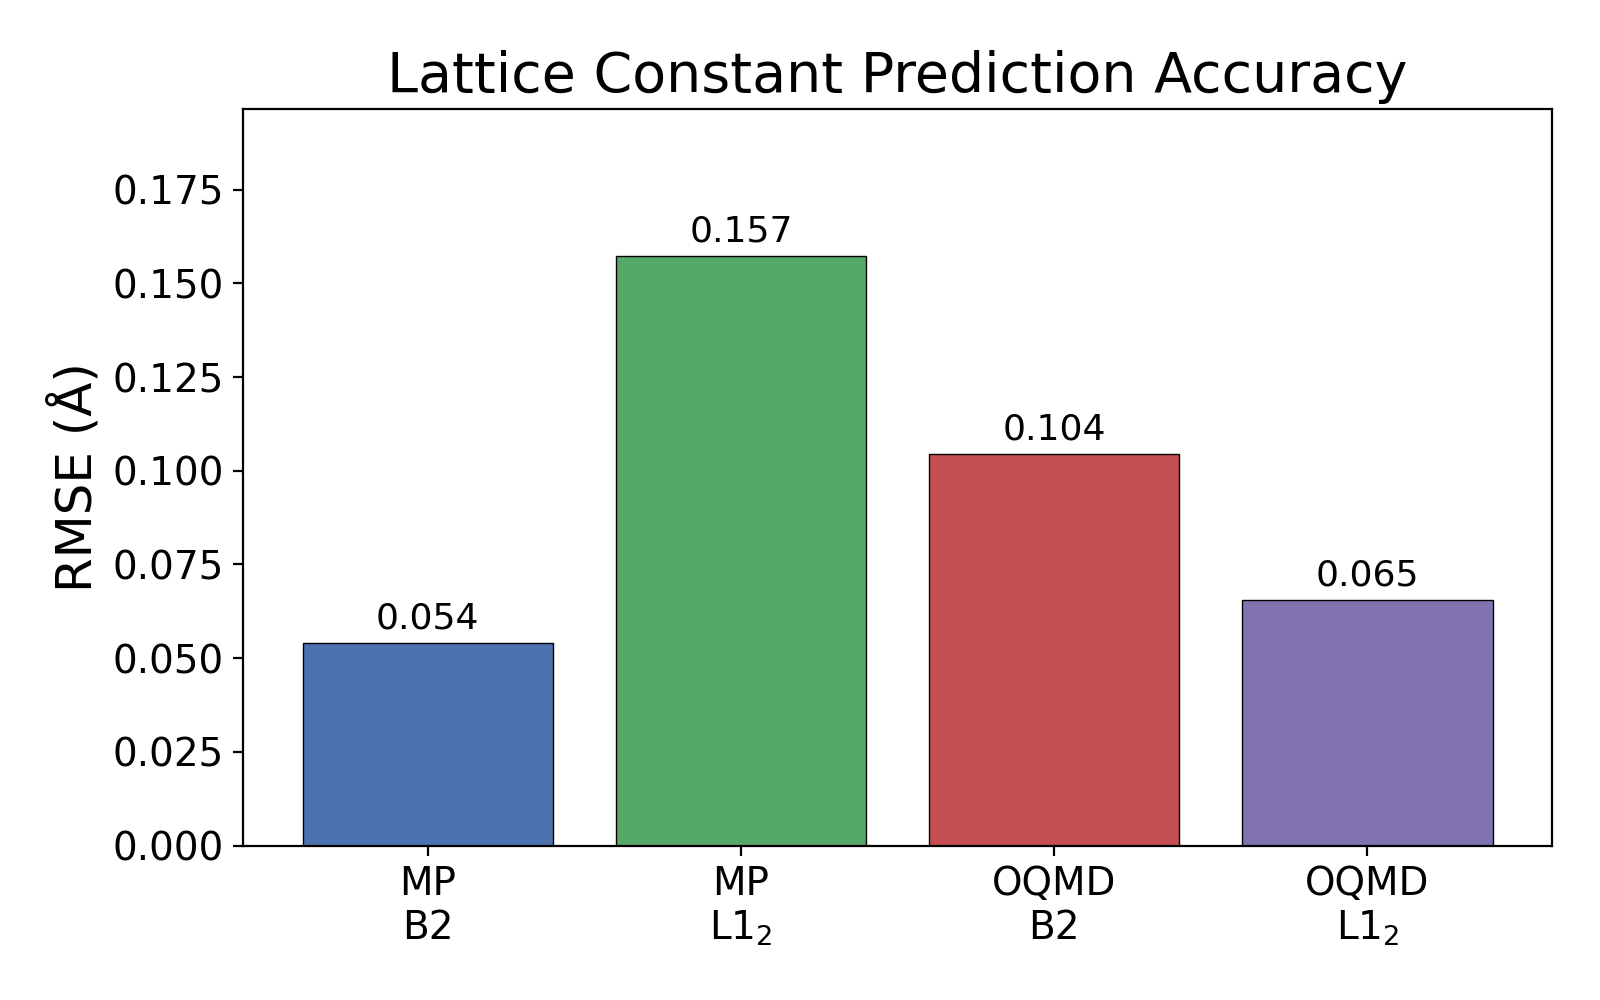
\includegraphics[width=0.45\textwidth]{12_model_performance.png}
    \caption{データベース・構造タイプ別の格子定数予測精度（RMSE）の比較。MP-B2が最高精度（RMSE = 0.054~\AA）を示す。}
    \label{fig:performance}
\end{figure}


\subsection{パリティプロット}
観測値と予測値のパリティプロットを図~\ref{fig:parity}に示す。B2では対角線近傍に点が密集し、系統的偏差が小さいことを示している。一方、L1$_2$では全体として良好な一致を保つものの、B2よりも散らばりがやや大きい。これはL1$_2$で複数の接触条件が競合し得ること、および剛体球近似で捉えられない電子的寄与を反映している可能性がある。

\begin{figure*}[htbp]
    \centering
    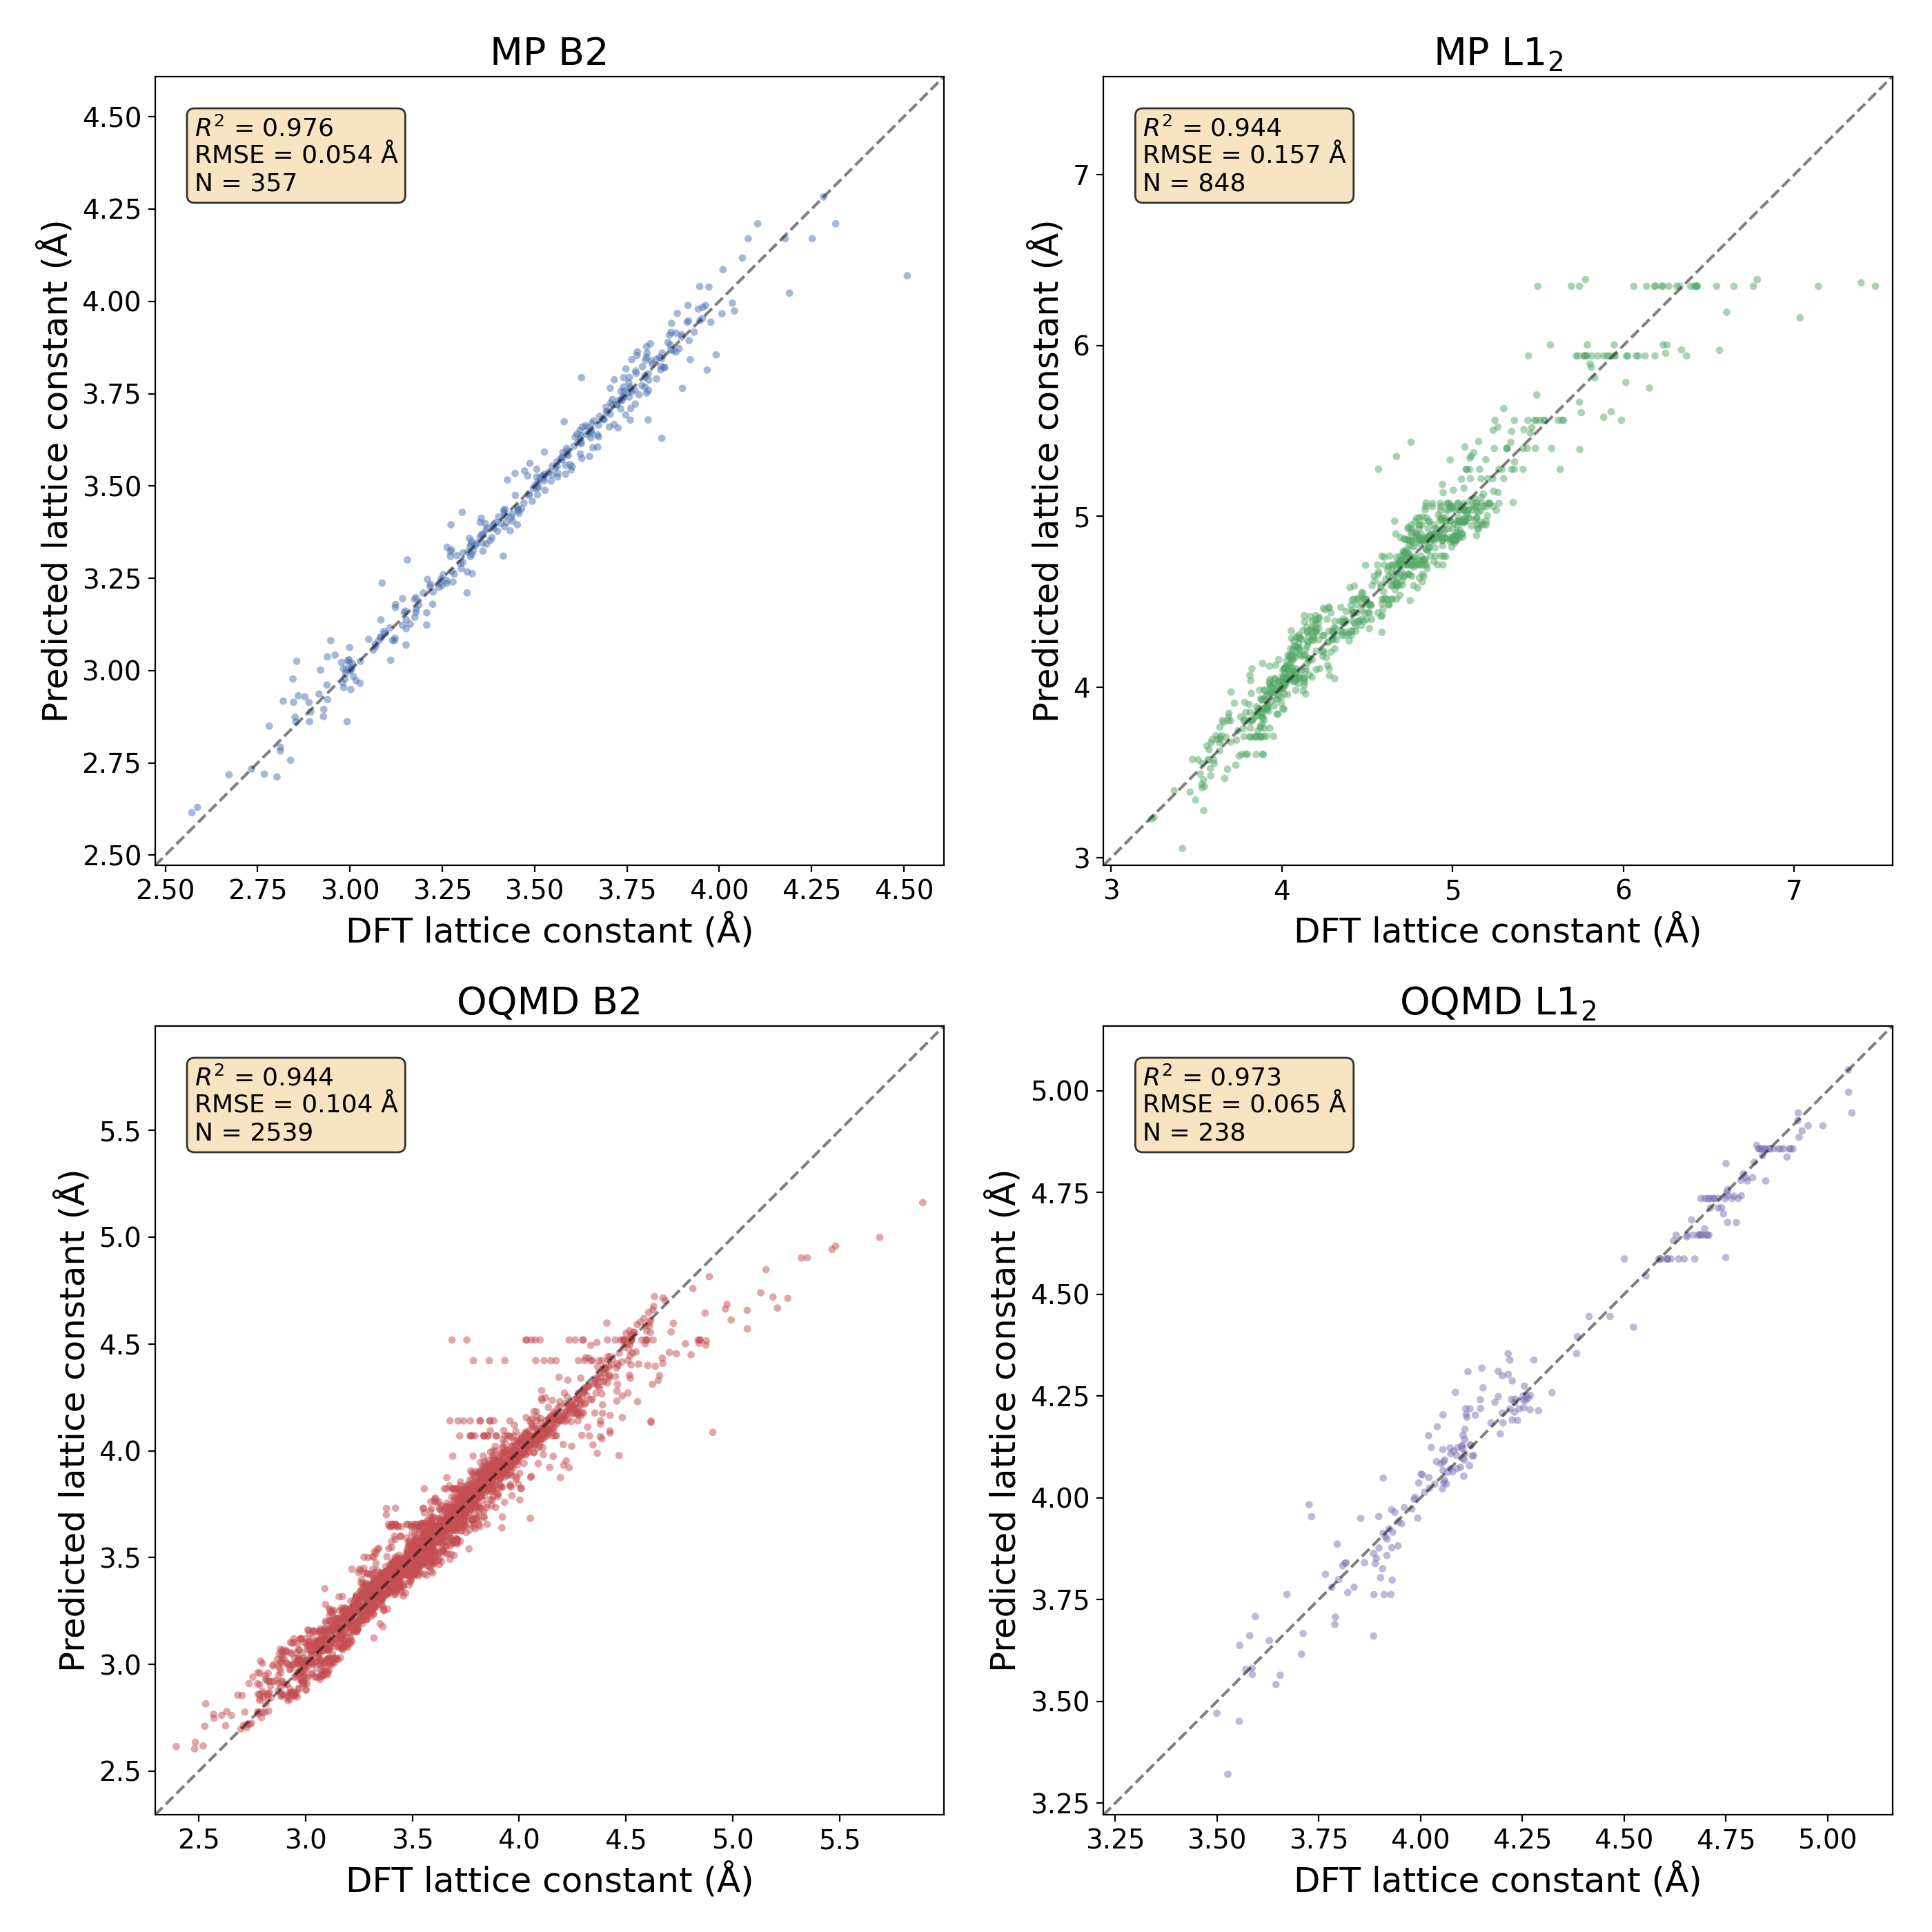
\includegraphics[width=0.85\textwidth]{oqmd_mp_common_parity.png}
    \caption{MP・OQMDの4ケースについて観測格子定数と予測格子定数のパリティプロット。破線は完全一致を示す。B2ではほぼ対角線上に集中し（RMSE = 0.054~\AA、$R^2 = 0.975$）、L1$_2$ではやや散らばりが大きい（RMSE = 0.116~\AA、$R^2 = 0.950$）。}
    \label{fig:parity}
\end{figure*}


\subsection{有効半径のBootstrap不確定性}
各元素の有効接触半径の不確定性をBootstrap法（1000回リサンプリング）により評価した結果を表~\ref{tab:bootstrap}にまとめた。半径の標準偏差の中央値はOQMD-B2で最小（0.007~\AA）、OQMD-L1$_2$で最大（0.021~\AA）であった。不確定性が大きい元素は各ケースで異なり、MP-B2ではFe（std = 0.052~\AA）、MP-L1$_2$ではBa（0.040~\AA）、OQMD-B2ではB（0.039~\AA）、OQMD-L1$_2$ではFe（0.060~\AA）が最大であった。OQMD-B2のstdが最小なのはデータ量（2539件）が多いことを反映している。

\begin{table*}[htbp]
\small
    \centering
    \caption{Bootstrap不確定性評価の要約（各ケース1000回リサンプリング）。有効接触半径の標準偏差の中央値・最大値、95\%信頼区間の平均幅を示す。}
    \label{tab:bootstrap}
    \begin{tabular}{lcccc}
        \toprule
        ケース & 中央値 std (\AA) & 最大 std (\AA) & 平均 95\% CI (\AA) & 最大 std 元素 \\
        \midrule
        MP-B2 & 0.014 & 0.052 & 0.065 & Fe \\
        MP-L1$_2$ & 0.017 & 0.040 & 0.070 & Ba \\
        OQMD-B2 & 0.007 & 0.039 & 0.036 & B \\
        OQMD-L1$_2$ & 0.021 & 0.060 & 0.094 & Fe \\
        \bottomrule
    \end{tabular}
\end{table*}


\subsection{古典的半径との比較}

\subsubsection{Goldschmidt半径との比較}
最適化されたL1$_2$半径は、Goldschmidt半径と良好な相関を示す（$R^2 = 0.946$、RMSE = 0.083~\AA）。L1$_2$は最密充填誘導体構造であり主成分原子は12個の最近接原子を持つため、配位数12の純金属から導かれたGoldschmidtの経験値との対応は物理的に合理的である。

\subsubsection{Pauling半径との比較}
B2半径とPauling半径の比較では$R^2 = 0.913$の相関が得られた。max基準モデルにおいて同種原子間接触（A-AまたはB-B）が支配的な化合物では、非支配的な原子種の半径は格子定数に直接影響しないため、その最適化に対する制約が弱まる。これは、B2有効半径が単なる古典的金属半径の写像ではなく、接触条件の切り替わりを含む構造特異的パラメータであることを示している。

\begin{figure*}[t]
  \centering
  \begin{minipage}[t]{0.48\textwidth}
    \centering
    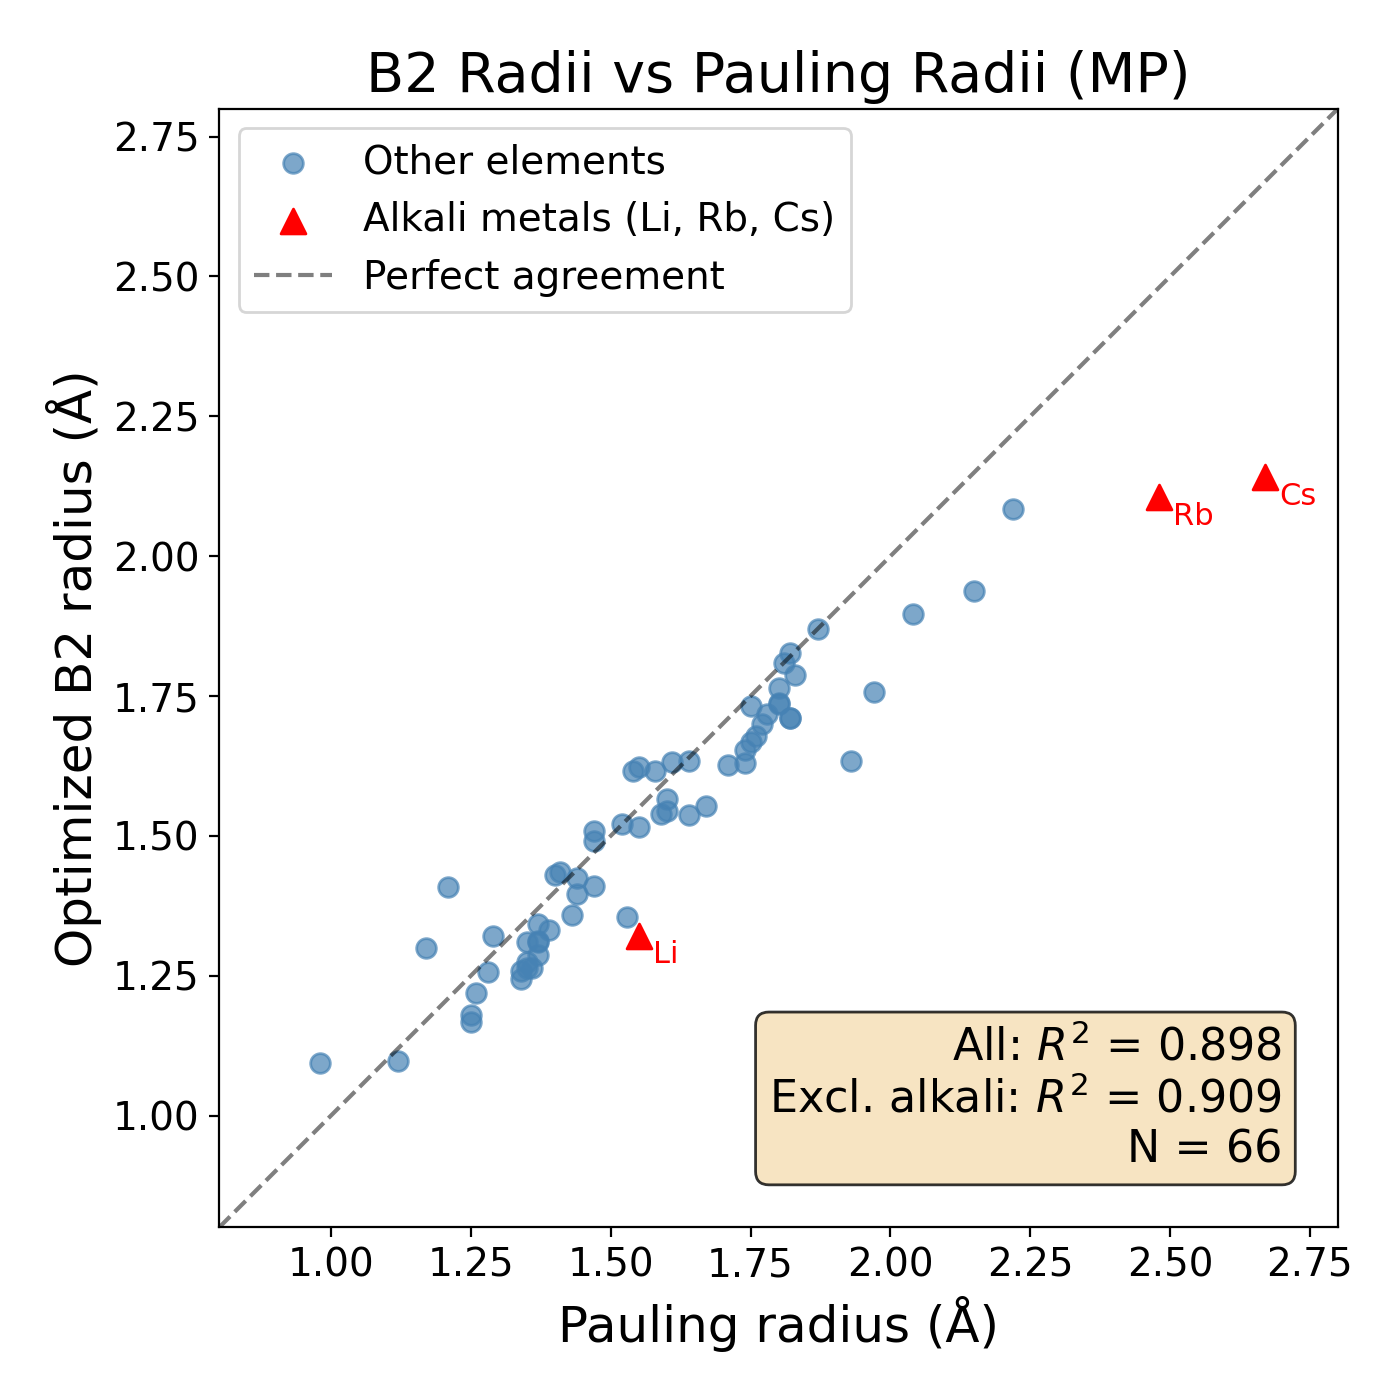
\includegraphics[width=0.9\textwidth]{05_B2_vs_pauling.png}
    \caption{最適化B2半径（MP）とPauling金属半径の比較。$R^2 = 0.913$。}
    \label{fig:B2_pauling}
  \end{minipage}
  \hfill
  \begin{minipage}[t]{0.48\textwidth}
    \centering
    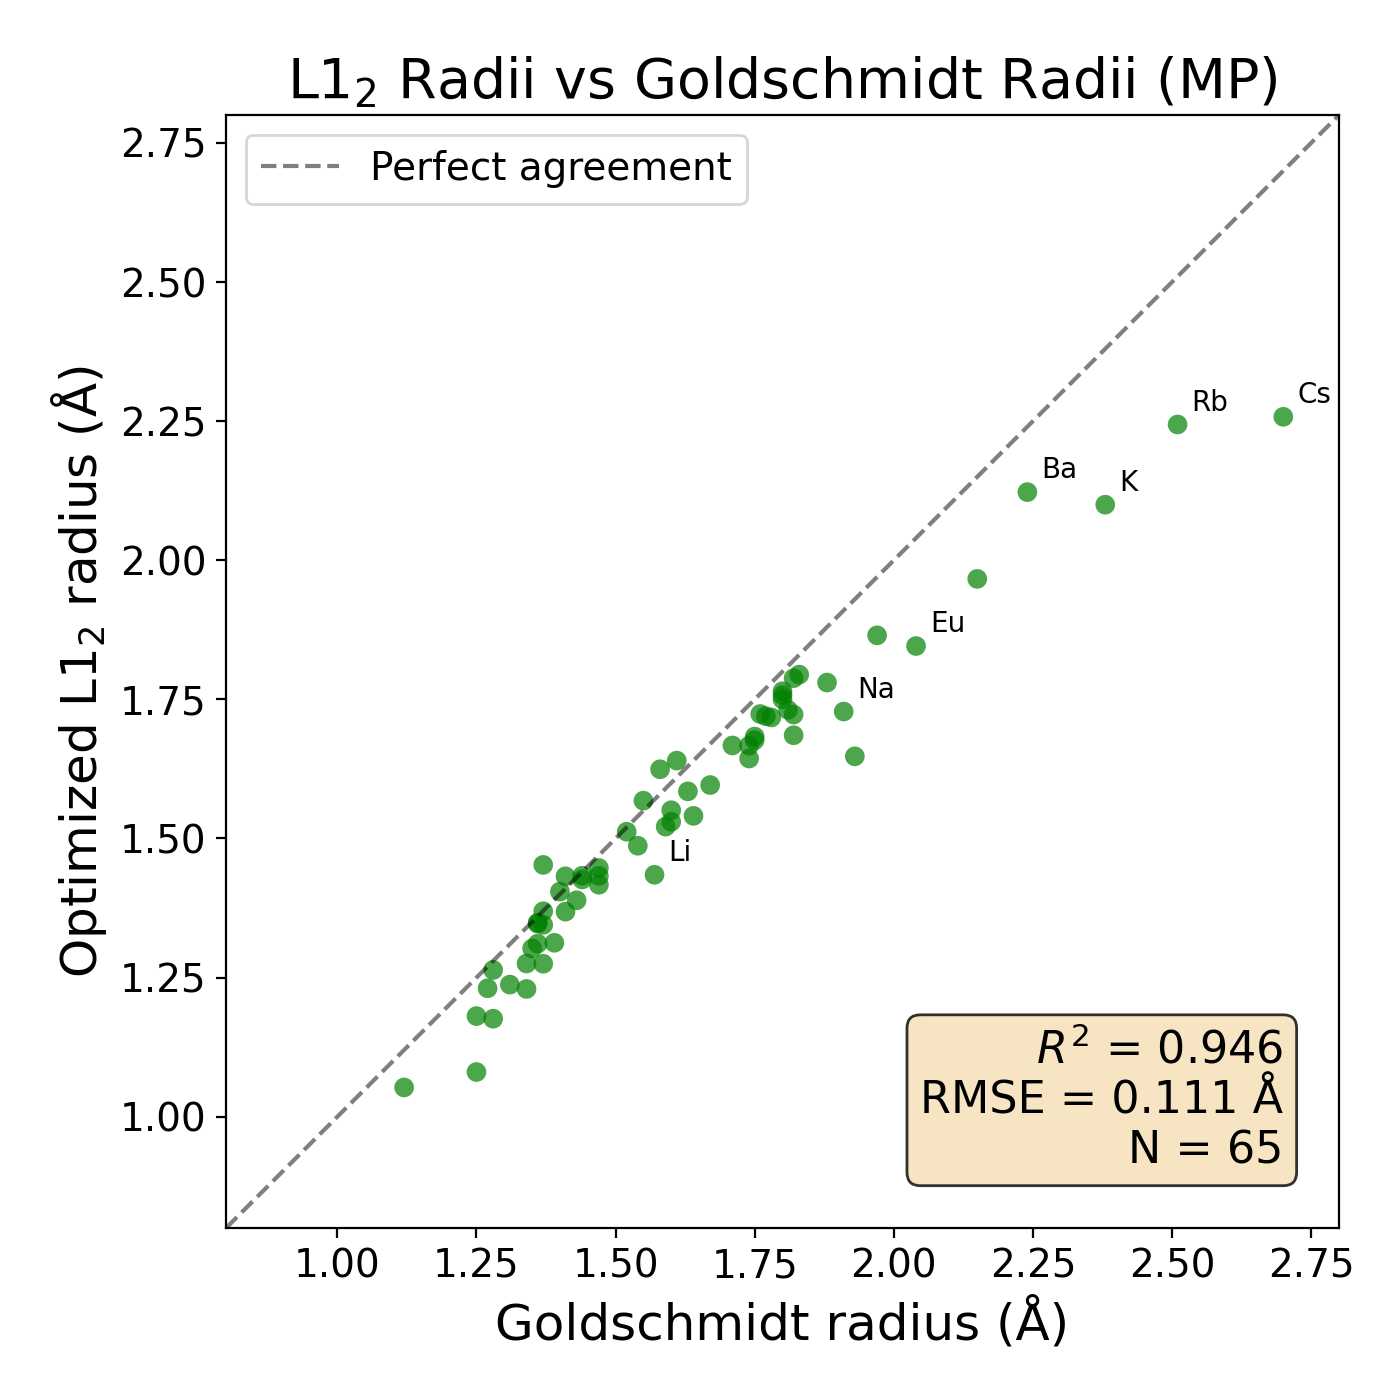
\includegraphics[width=0.9\textwidth]{gs_02_L12_vs_goldschmidt.png}
    \caption{最適化L1$_2$半径（MP）とGoldschmidt金属半径の比較。$R^2 = 0.946$。}
    \label{fig:L12_goldschmidt}    
  \end{minipage}
\end{figure*}


\subsection{B2--L1$_2$半径差の解析}
B2構造（CN=8）とL1$_2$構造（CN=12）の間で原子半径がどれだけ変化するかは重要な問題である。Goldschmidtの経験則によれば、配位数が12から8に変化すると半径は約3\%縮小すると考えられる。

表~\ref{tab:top_contraction}に、MPデータセットにおけるB2--L1$_2$半径差の上位・下位元素を示す。最大の収縮を示すのはRe（$-5.9$\%）、次いでCa（$-5.6$\%）。逆にNi（$+7.9$\%）やPu（$+7.4$\%）はB2半径がL1$_2$半径より大きい傾向を示す。

\begin{table*}[htbp]
\small
    \centering
    \caption{MPデータセットにおけるB2--L1$_2$半径差の上位・下位元素。負の値はB2半径がL1$_2$半径より小さいことを示す。}
    \label{tab:top_contraction}
\scalebox{0.9}{
    \begin{tabular}{lccccc}
        \toprule
        元素 & B2半径 (\AA) & L1$_2$半径 (\AA) & 差 (\AA) & 収縮率 (\%) & 元素群 \\
        \midrule
        Re & 1.29 & 1.37 & $-$0.08 & $-$5.9 & 5d遷移金属 \\
        Ca & 1.75 & 1.86 & $-$0.10 & $-$5.6 & アルカリ土類 \\
        Hg & 1.52 & 1.57 & $-$0.06 & $-$3.6 & 5d遷移金属 \\
        Ir & 1.27 & 1.31 & $-$0.04 & $-$3.4 & 5d遷移金属 \\
        Ga & 1.35 & 1.40 & $-$0.05 & $-$3.4 & 遷移後金属 \\
        \midrule
        Ce & 1.79 & 1.69 & $+$0.10 & $+$6.0 & ランタノイド \\
        Mn & 1.31 & 1.23 & $+$0.08 & $+$6.4 & 3d遷移金属 \\
        U & 1.62 & 1.52 & $+$0.10 & $+$6.5 & アクチノイド \\
        Pu & 1.63 & 1.52 & $+$0.11 & $+$7.4 & アクチノイド \\
        Ni & 1.18 & 1.09 & $+$0.09 & $+$7.9 & 3d遷移金属 \\
        \bottomrule
    \end{tabular}
    }
\end{table*}

B2--L1$_2$収縮率の分布を図~\ref{fig:B2_contraction}に示す。Goldschmidtの3\%ルール（赤破線）との比較では、遷移金属の大半が0--5\%の範囲に収まるが、分布は非対称であり、B2 $<$ L1$_2$（負側）に長い裾を持つ。

\begin{figure}[htbp]
    \centering
    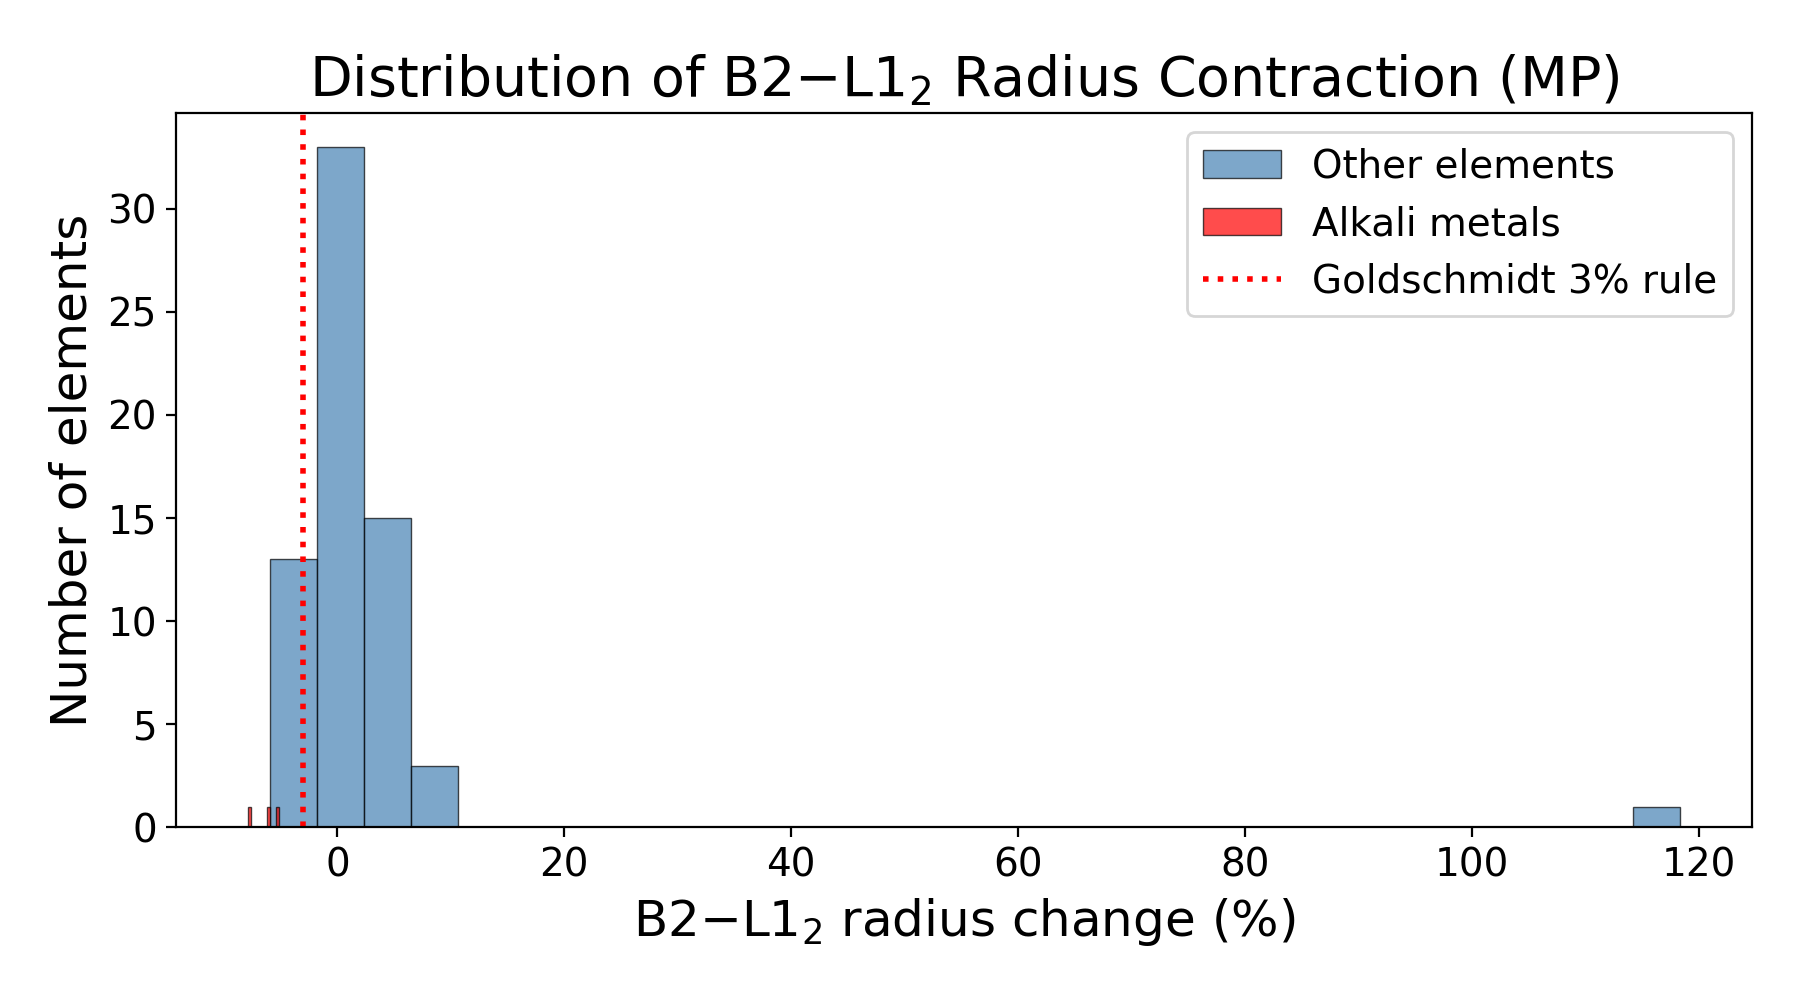
\includegraphics[width=0.45\textwidth]{gs_04_B2_contraction.png}
    \caption{B2--L1$_2$半径収縮率の分布（MP）。赤破線はGoldschmidtの3\%収縮予測。遷移金属の大部分はこの値付近に分布する。}
    \label{fig:B2_contraction}
\end{figure}


\subsection{元素群別解析}
有効半径の体系的傾向をみるため、元素をアルカリ土類、3d/4d/5d遷移金属、ランタノイド、アクチノイド、遷移後金属に分類してB2--L1$_2$差を比較した。表~\ref{tab:element_groups}に示すように、3d遷移金属の平均変化率は$+1.7$\%、5d遷移金属は$-0.3$\%であり、周期律表の下方へ行くほど収縮傾向が現れる。アクチノイドは$+4.1$\%とB2側への膨張が大きい。

\begin{table*}[htbp]
\small
    \centering
    \caption{元素群別のB2--L1$_2$半径収縮統計（MPデータ）。「平均」は群内の平均収縮率、「範囲」は最小--最大値を示す。}
    \label{tab:element_groups}
\scalebox{0.9}{
    \begin{tabular}{lcccccc}
        \toprule
        元素群 & N & B2平均 (\AA) & L1$_2$平均 (\AA) & 平均 (\%) & 範囲 (\%) & 特徴 \\
        \midrule
        アルカリ土類 & 5 & 1.68 & 1.69 & $-$0.2 & $-$5.6 $\sim$ $+$3.7 & Ca収縮 \\
        3d遷移金属 & 10 & 1.30 & 1.28 & $+$1.7 & $-$2.8 $\sim$ $+$7.9 & Ni膨張 \\
        4d遷移金属 & 10 & 1.43 & 1.42 & $+$0.7 & $-$2.0 $\sim$ $+$4.0 & 混合 \\
        5d遷移金属 & 10 & 1.44 & 1.44 & $-$0.3 & $-$5.9 $\sim$ $+$5.3 & Re収縮 \\
        ランタノイド & 14 & 1.73 & 1.73 & $+$0.5 & $-$2.2 $\sim$ $+$6.0 & 微小膨張 \\
        アクチノイド & 5 & 1.72 & 1.65 & $+$4.1 & $-$1.3 $\sim$ $+$7.4 & B2膨張 \\
        遷移後金属 & 6 & 1.54 & 1.57 & $-$1.9 & $-$3.4 $\sim$ $-$0.5 & 中程度収縮 \\
        \bottomrule
    \end{tabular}
    }
\end{table*}


\subsection{データベース間の整合性}
両データベースに共通する化合物について比較した結果、B2では346件、L1$_2$では183件の共通化合物が存在した。格子定数の比較ではB2で$R^2 = 0.986$、L1$_2$で$R^2 = 0.986$と高い整合性が認められた。有効半径についてもB2では$R^2 = 0.958$（64共通元素）と高い整合性が確認された。L1$_2$の半径整合性は$R^2 = 0.875$（56共通元素）であり、B2よりやや低いが、OQMDのL1$_2$データ数（238件）がMP（848件）より少ないことが一因である。

\begin{table}[htbp]
\small
    \centering
    \caption{MPとOQMDの共通化合物における整合性。}
    \label{tab:consistency}
\scalebox{0.9}{
    \begin{tabular}{lcccc}
        \toprule
        構造 & 共通化合物数 & 格子定数 $R^2$ & 共通元素数 & 半径 $R^2$ \\
        \midrule
        B2 & 346 & 0.986 & 64 & 0.958 \\
        L1$_2$ & 183 & 0.986 & 56 & 0.875 \\
        \bottomrule
    \end{tabular}
    }
\end{table}

\begin{figure*}[t]
  \centering
  \begin{minipage}[t]{0.48\textwidth}
    \centering
    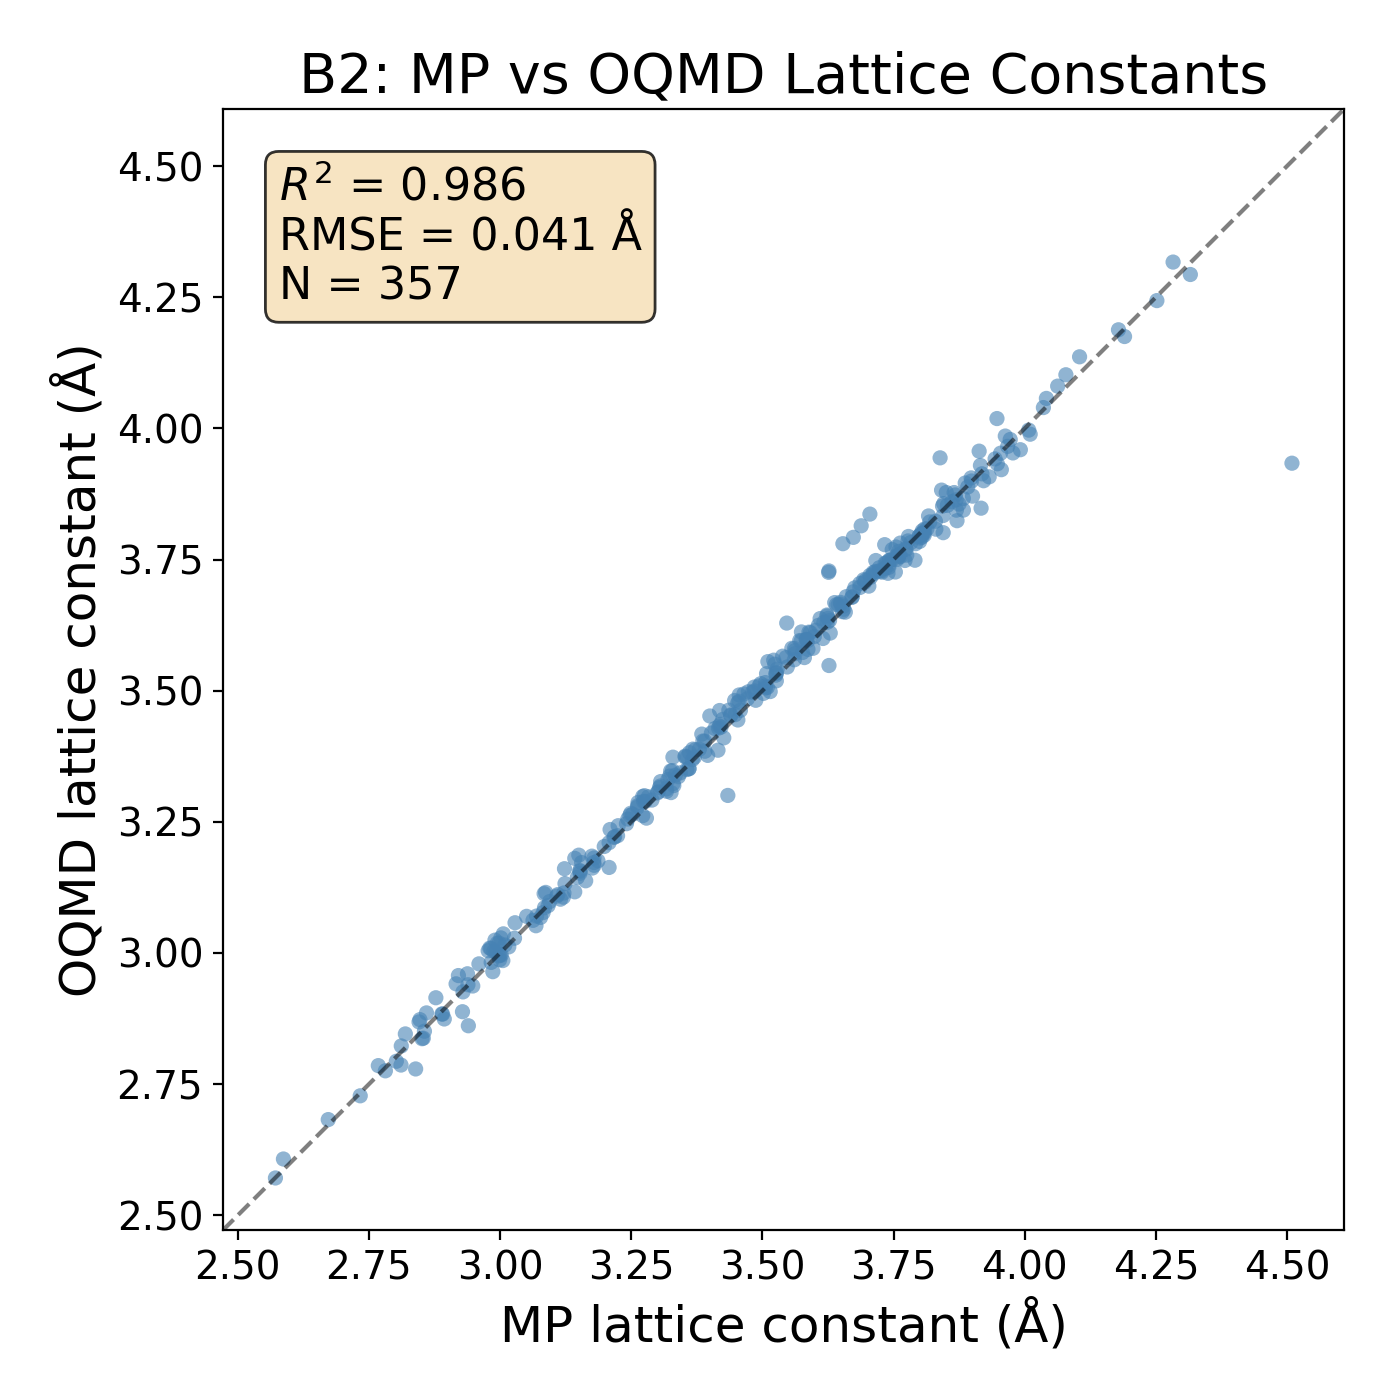
\includegraphics[width=0.9\linewidth]{a7_common_B2.png}
    \caption{MPとOQMDの共通B2化合物（346件）の格子定数比較。$R^2 = 0.986$。}
    \label{fig:common_B2}
  \end{minipage}
  \hfill
  \begin{minipage}[t]{0.48\textwidth}
    \centering
    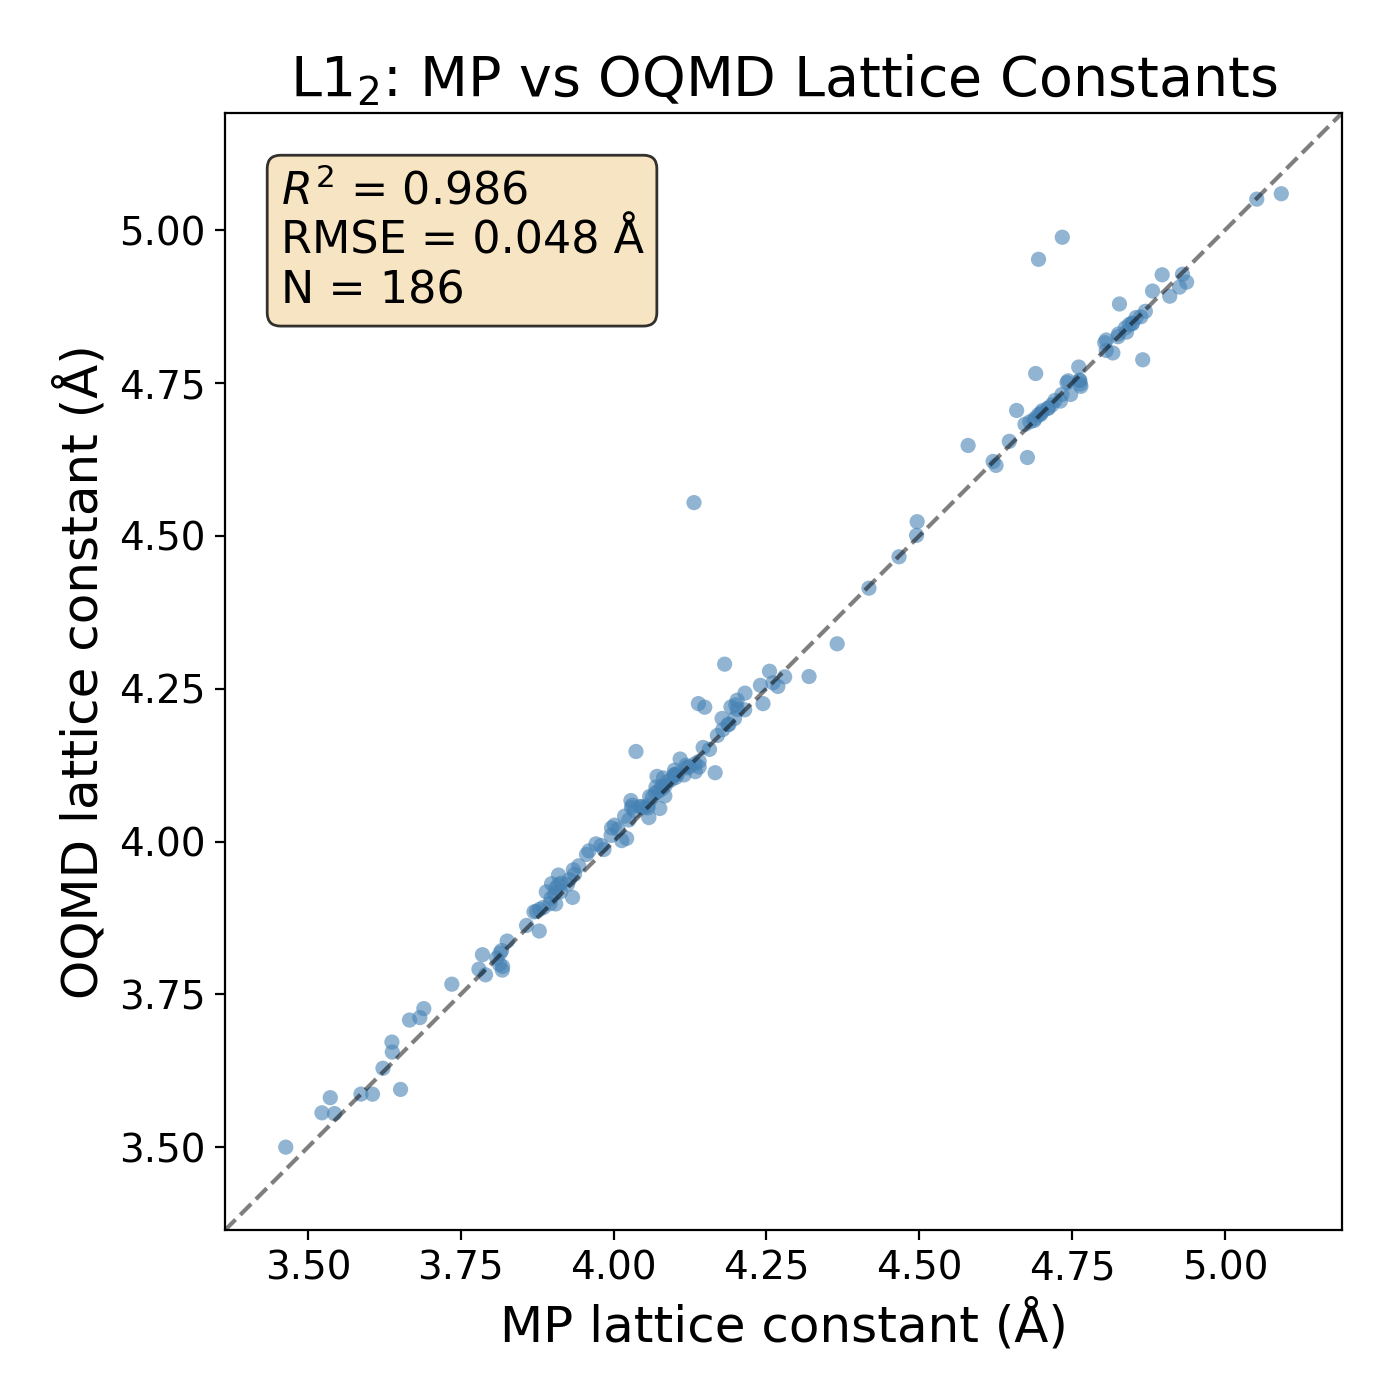
\includegraphics[width=0.9\linewidth]{a7_common_L12.png}
    \caption{MPとOQMDの共通L1$_2$化合物（183件）の格子定数比較。$R^2 = 0.986$。}
    \label{fig:common_L12}
  \end{minipage}
\end{figure*}


\subsection{疑似Vegard則解析}

\subsubsection{3つの指標の比較}
52の二元系（3組成すべてのデータが揃うペア）について、3つの指標で疑似Vegard則の線形性を検証した。図~\ref{fig:three_metrics}に代表12ペアについての結果を示す。

\begin{figure*}[htbp]
    \centering
    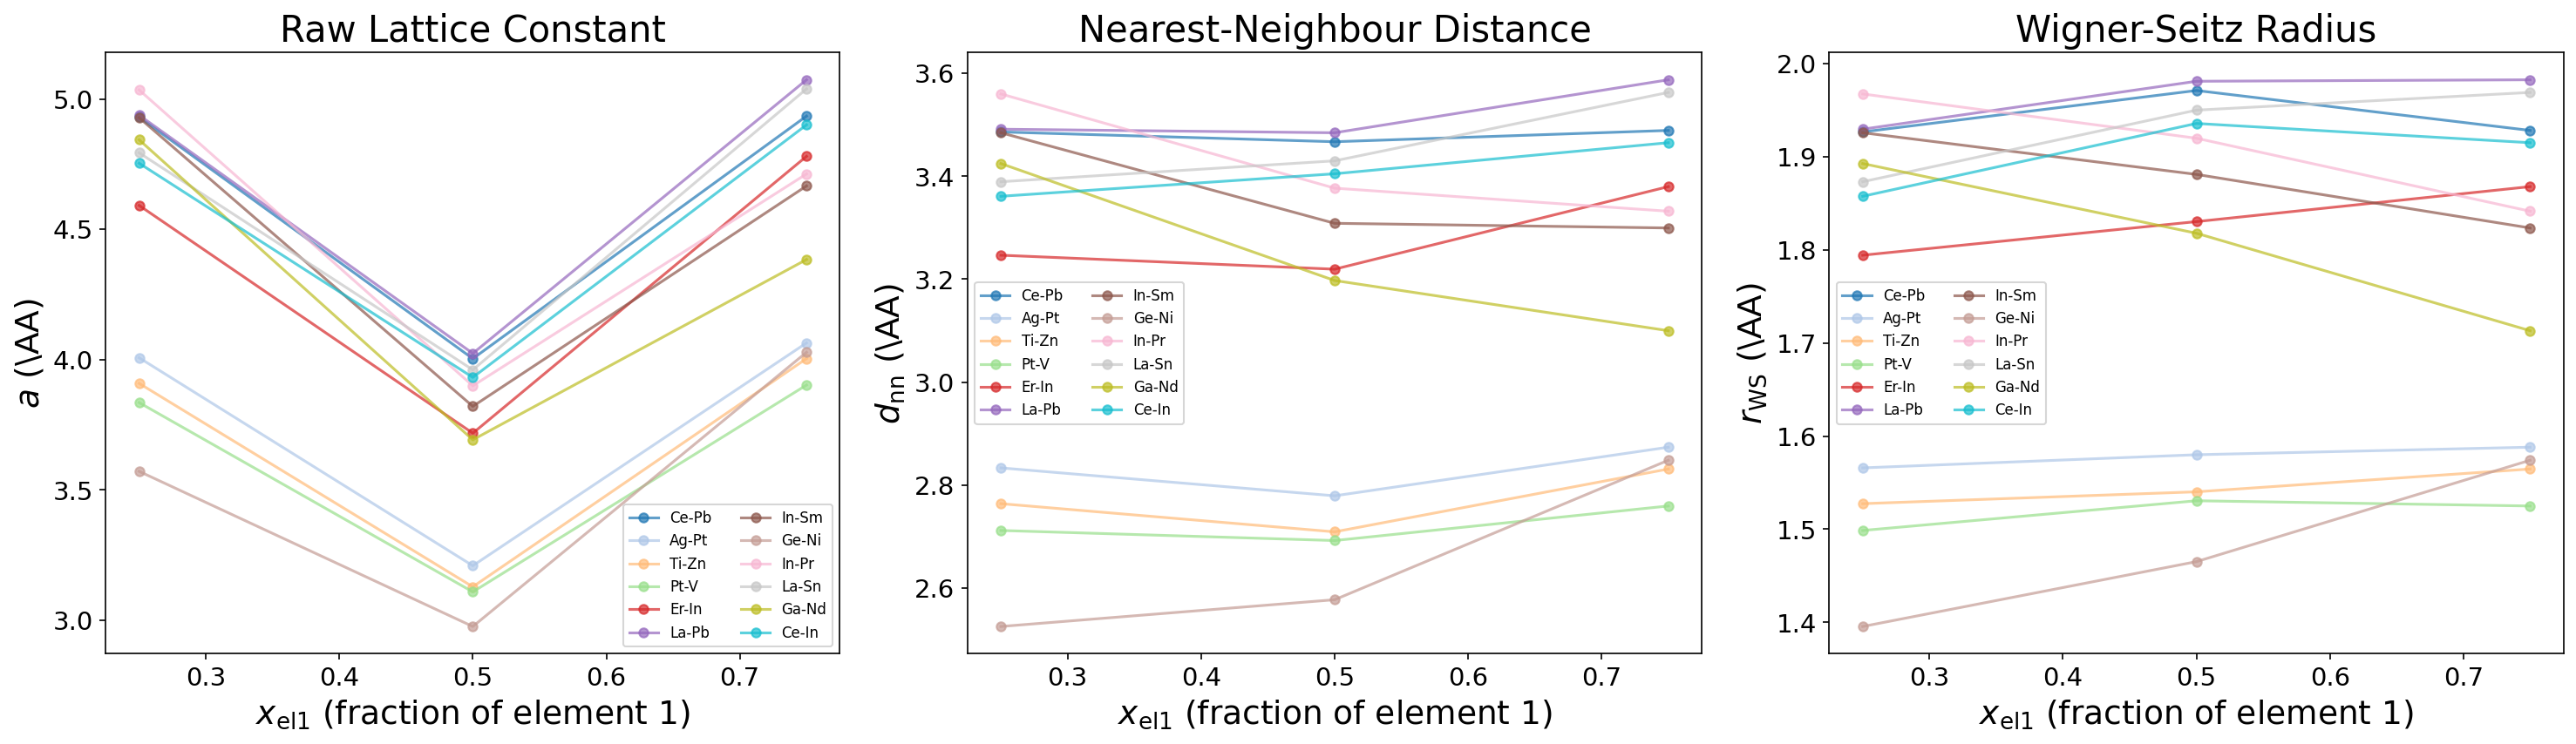
\includegraphics[width=0.95\textwidth]{vegard_three_metrics.png}
    \caption{代表12ペアについて3つの指標（生の格子定数$a$、最近接原子間距離$d_\mathrm{nn}$、Wigner--Seitz半径$r_\mathrm{WS}$）で描いた疑似Vegard則プロット。横軸はA元素の組成分率。左パネルでは50\%点（B2）が大きく凹む「V字型」となるが、右パネル（$r_\mathrm{WS}$）ではほぼ直線に乗る。}
    \label{fig:three_metrics}
\end{figure*}

\begin{itemize}
\setlength{\parskip}{0cm}
\setlength{\itemsep}{0cm}
    \item \textbf{生の格子定数$a$}: B2（$a \sim 3$~\AA）とL1$_2$（$a \sim 4$~\AA）でスケールが全く異なるため、50\%点が大きく凹む「V字型」となり、中央値$R^2 = 0.036$とほぼ線形性を示さない。
    \item \textbf{最近接原子間距離$d_\mathrm{nn}$}: V字がかなり緩和されるが、50\%点が直線からずれるペアが多い。中央値$R^2 = 0.778$と中程度の線形性。
    \item \textbf{Wigner--Seitz半径$r_\mathrm{WS}$}: 3点がほぼ直線に乗る。中央値$R^2 = 0.974$と非常に高い線形性を示し、52ペア中32ペアが$R^2 > 0.95$。
\end{itemize}

\subsubsection{$R^2$分布の比較}
図~\ref{fig:r2_histogram}に$r_\mathrm{WS}$版の$R^2$ヒストグラムを示す。$R^2 > 0.95$に巨大なピークが集中しており、大多数のペアで$R^2 \approx 1$に収束している。$d_\mathrm{nn}$版では分布が広く散らばるのと対照的である。

\begin{figure}[htbp]
    \centering
    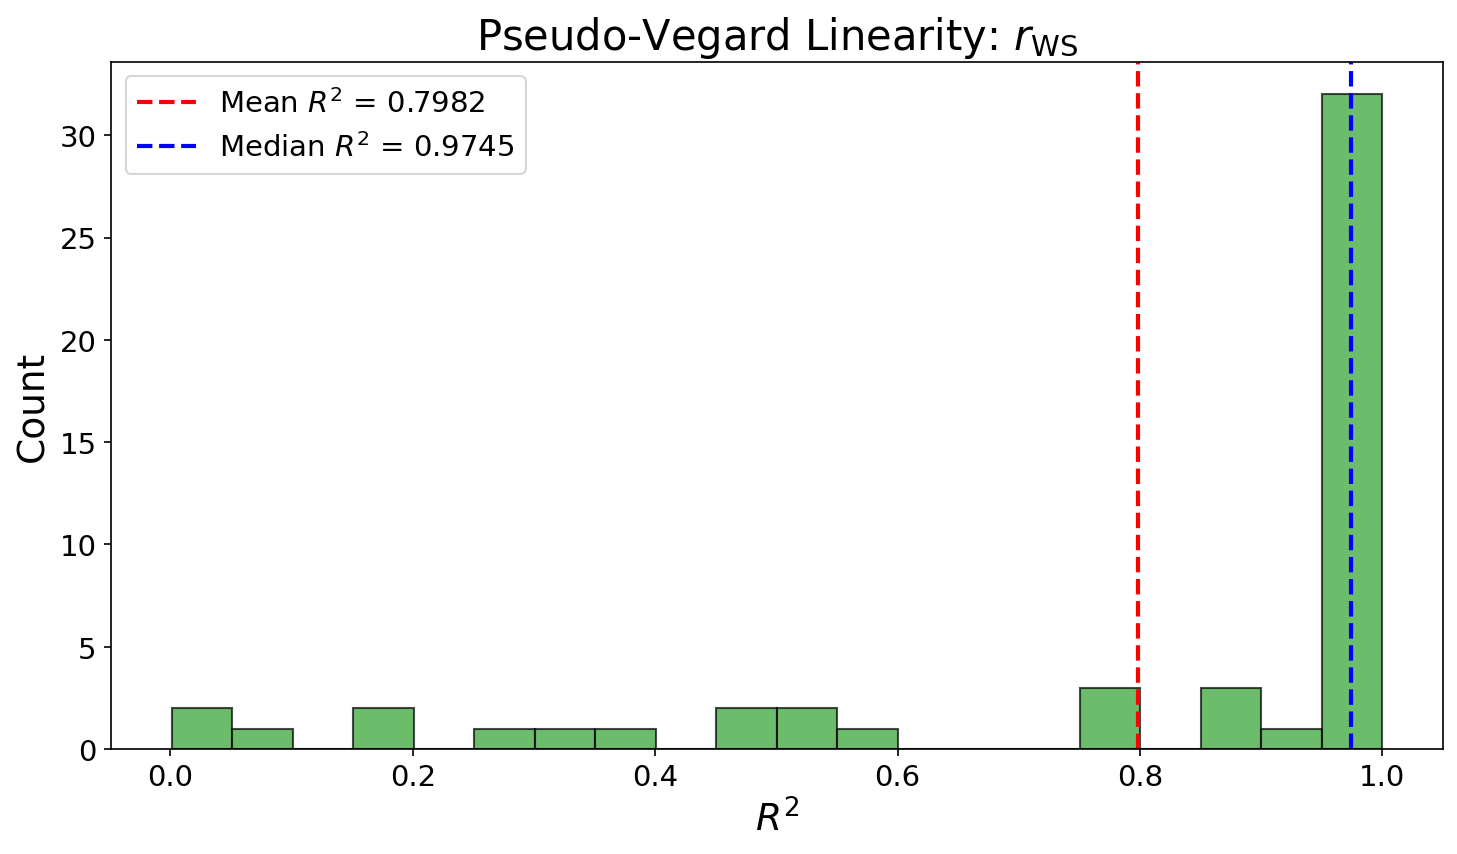
\includegraphics[width=0.45\textwidth]{vegard_r2_histogram_rws.png}
    \caption{$r_\mathrm{WS}$指標による52ペアの$R^2$ヒストグラム。$R^2 > 0.95$に32ペアが集中。中央値 = 0.974。}
    \label{fig:r2_histogram}
\end{figure}

図~\ref{fig:r2_comparison}に$d_\mathrm{nn}$と$r_\mathrm{WS}$の$R^2$分布を並列で比較したヒストグラムを示す。$r_\mathrm{WS}$では右端に集中するのに対し、$d_\mathrm{nn}$では幅広く分布している。

\begin{figure}[htbp]
    \centering
    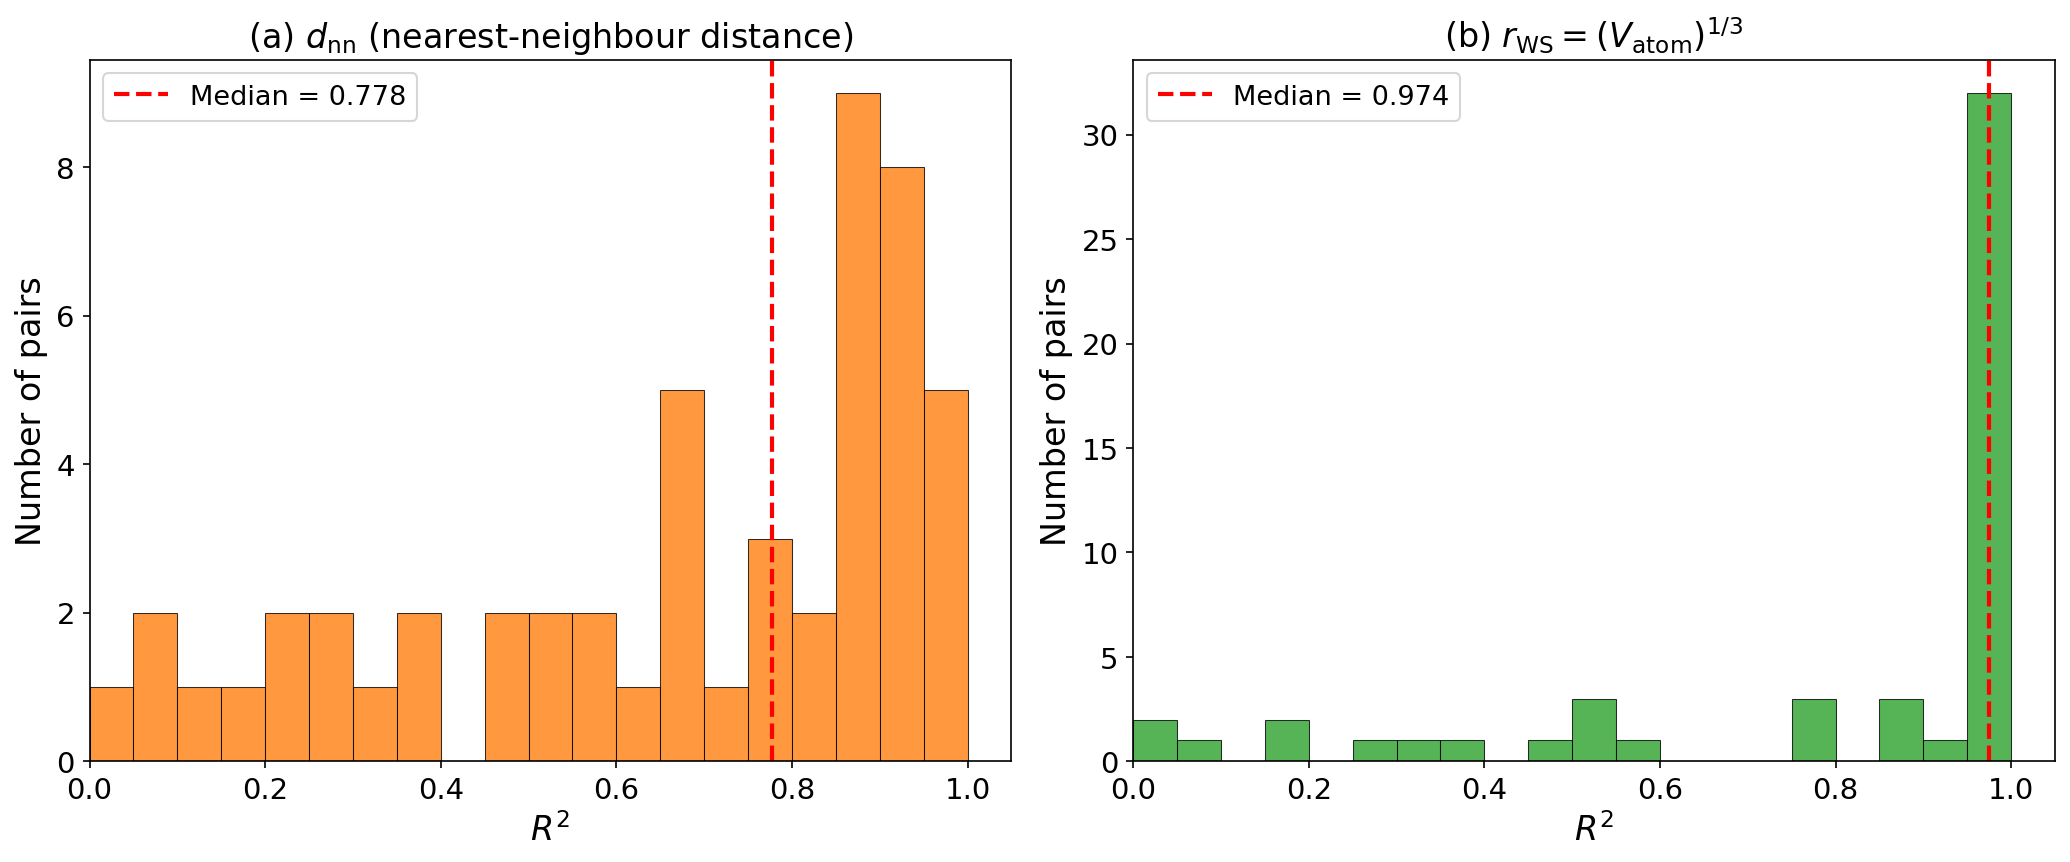
\includegraphics[width=0.45\textwidth]{vegard_r2_comparison_histogram.png}
    \caption{$d_\mathrm{nn}$（青）と$r_\mathrm{WS}$（赤）の$R^2$分布の比較。$r_\mathrm{WS}$指標が圧倒的に高い線形性を示す。}
    \label{fig:r2_comparison}
\end{figure}

\subsubsection{$R^2(r_\mathrm{WS})$ vs $R^2(d_\mathrm{nn})$散布図}
図~\ref{fig:r2_scatter}に52ペアについて$R^2(r_\mathrm{WS})$と$R^2(d_\mathrm{nn})$の散布図を示す。大多数の点が対角線より上（$r_\mathrm{WS}$の方が高い$R^2$）に位置し、原子体積ベースの指標が系統的に優れていることを確認できる。

\begin{figure}[htbp]
    \centering
    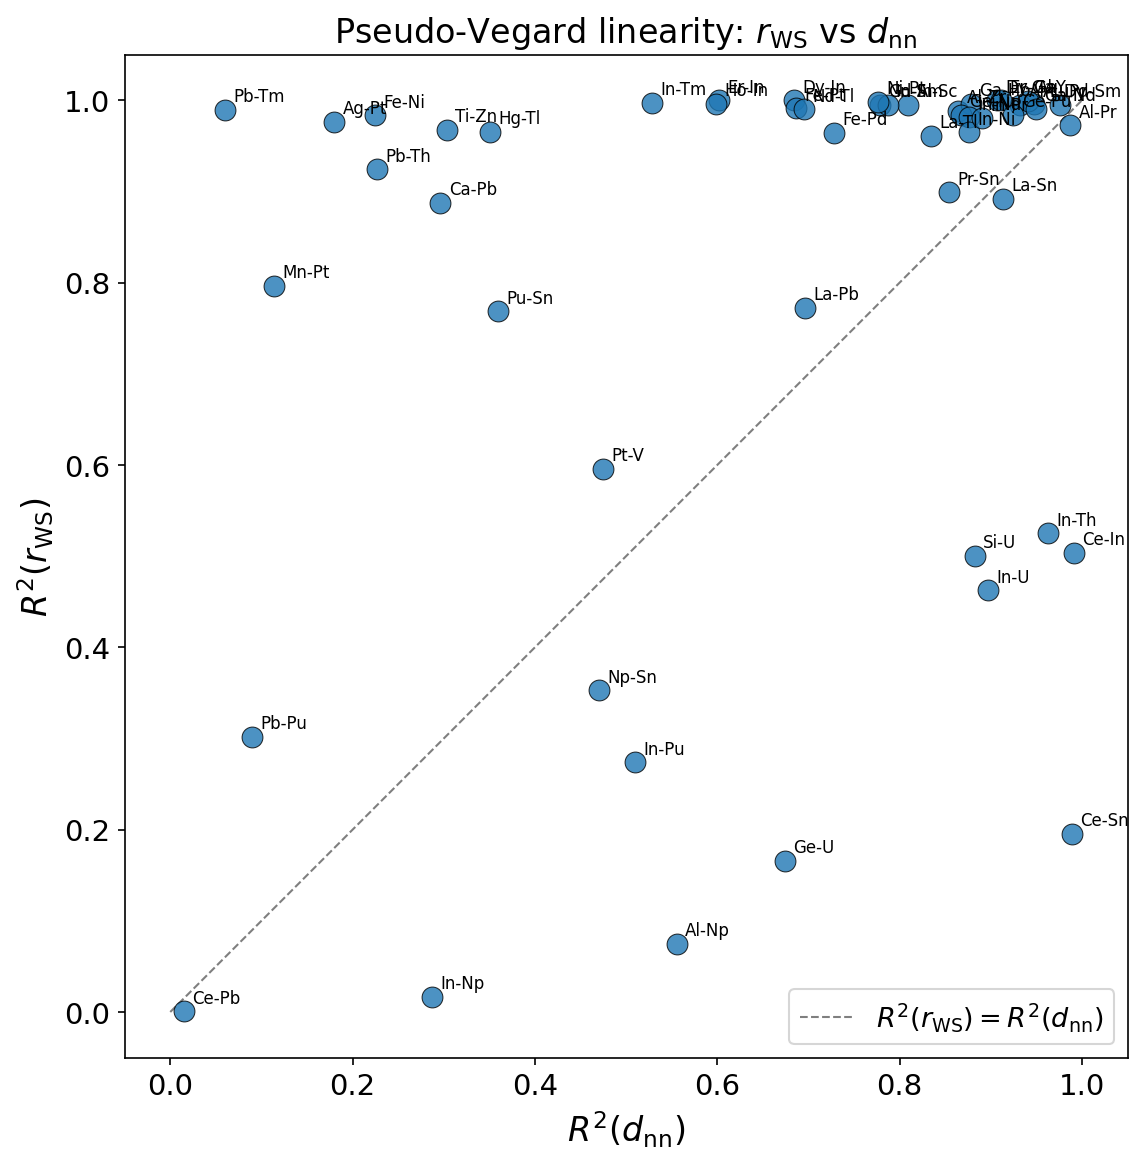
\includegraphics[width=0.45\textwidth]{vegard_r2_scatter_rws_vs_dnn.png}
    \caption{52ペアの$R^2(r_\mathrm{WS})$ vs $R^2(d_\mathrm{nn})$散布図。対角線より上は$r_\mathrm{WS}$指標が優れることを示す。}
    \label{fig:r2_scatter}
\end{figure}

\subsubsection{52ペアサマリーグリッド}
図~\ref{fig:triplet_summary}に、3組成すべてが揃った52ペアについて$r_\mathrm{WS}$で描いたサマリーグリッドを示す。$R^2$降順でソートされ、枠線の色でフィット品質を示す（緑: $>0.99$、青: $>0.95$、橙: $>0.90$、赤: $<0.90$）。

\begin{figure*}[htbp]
    \centering
    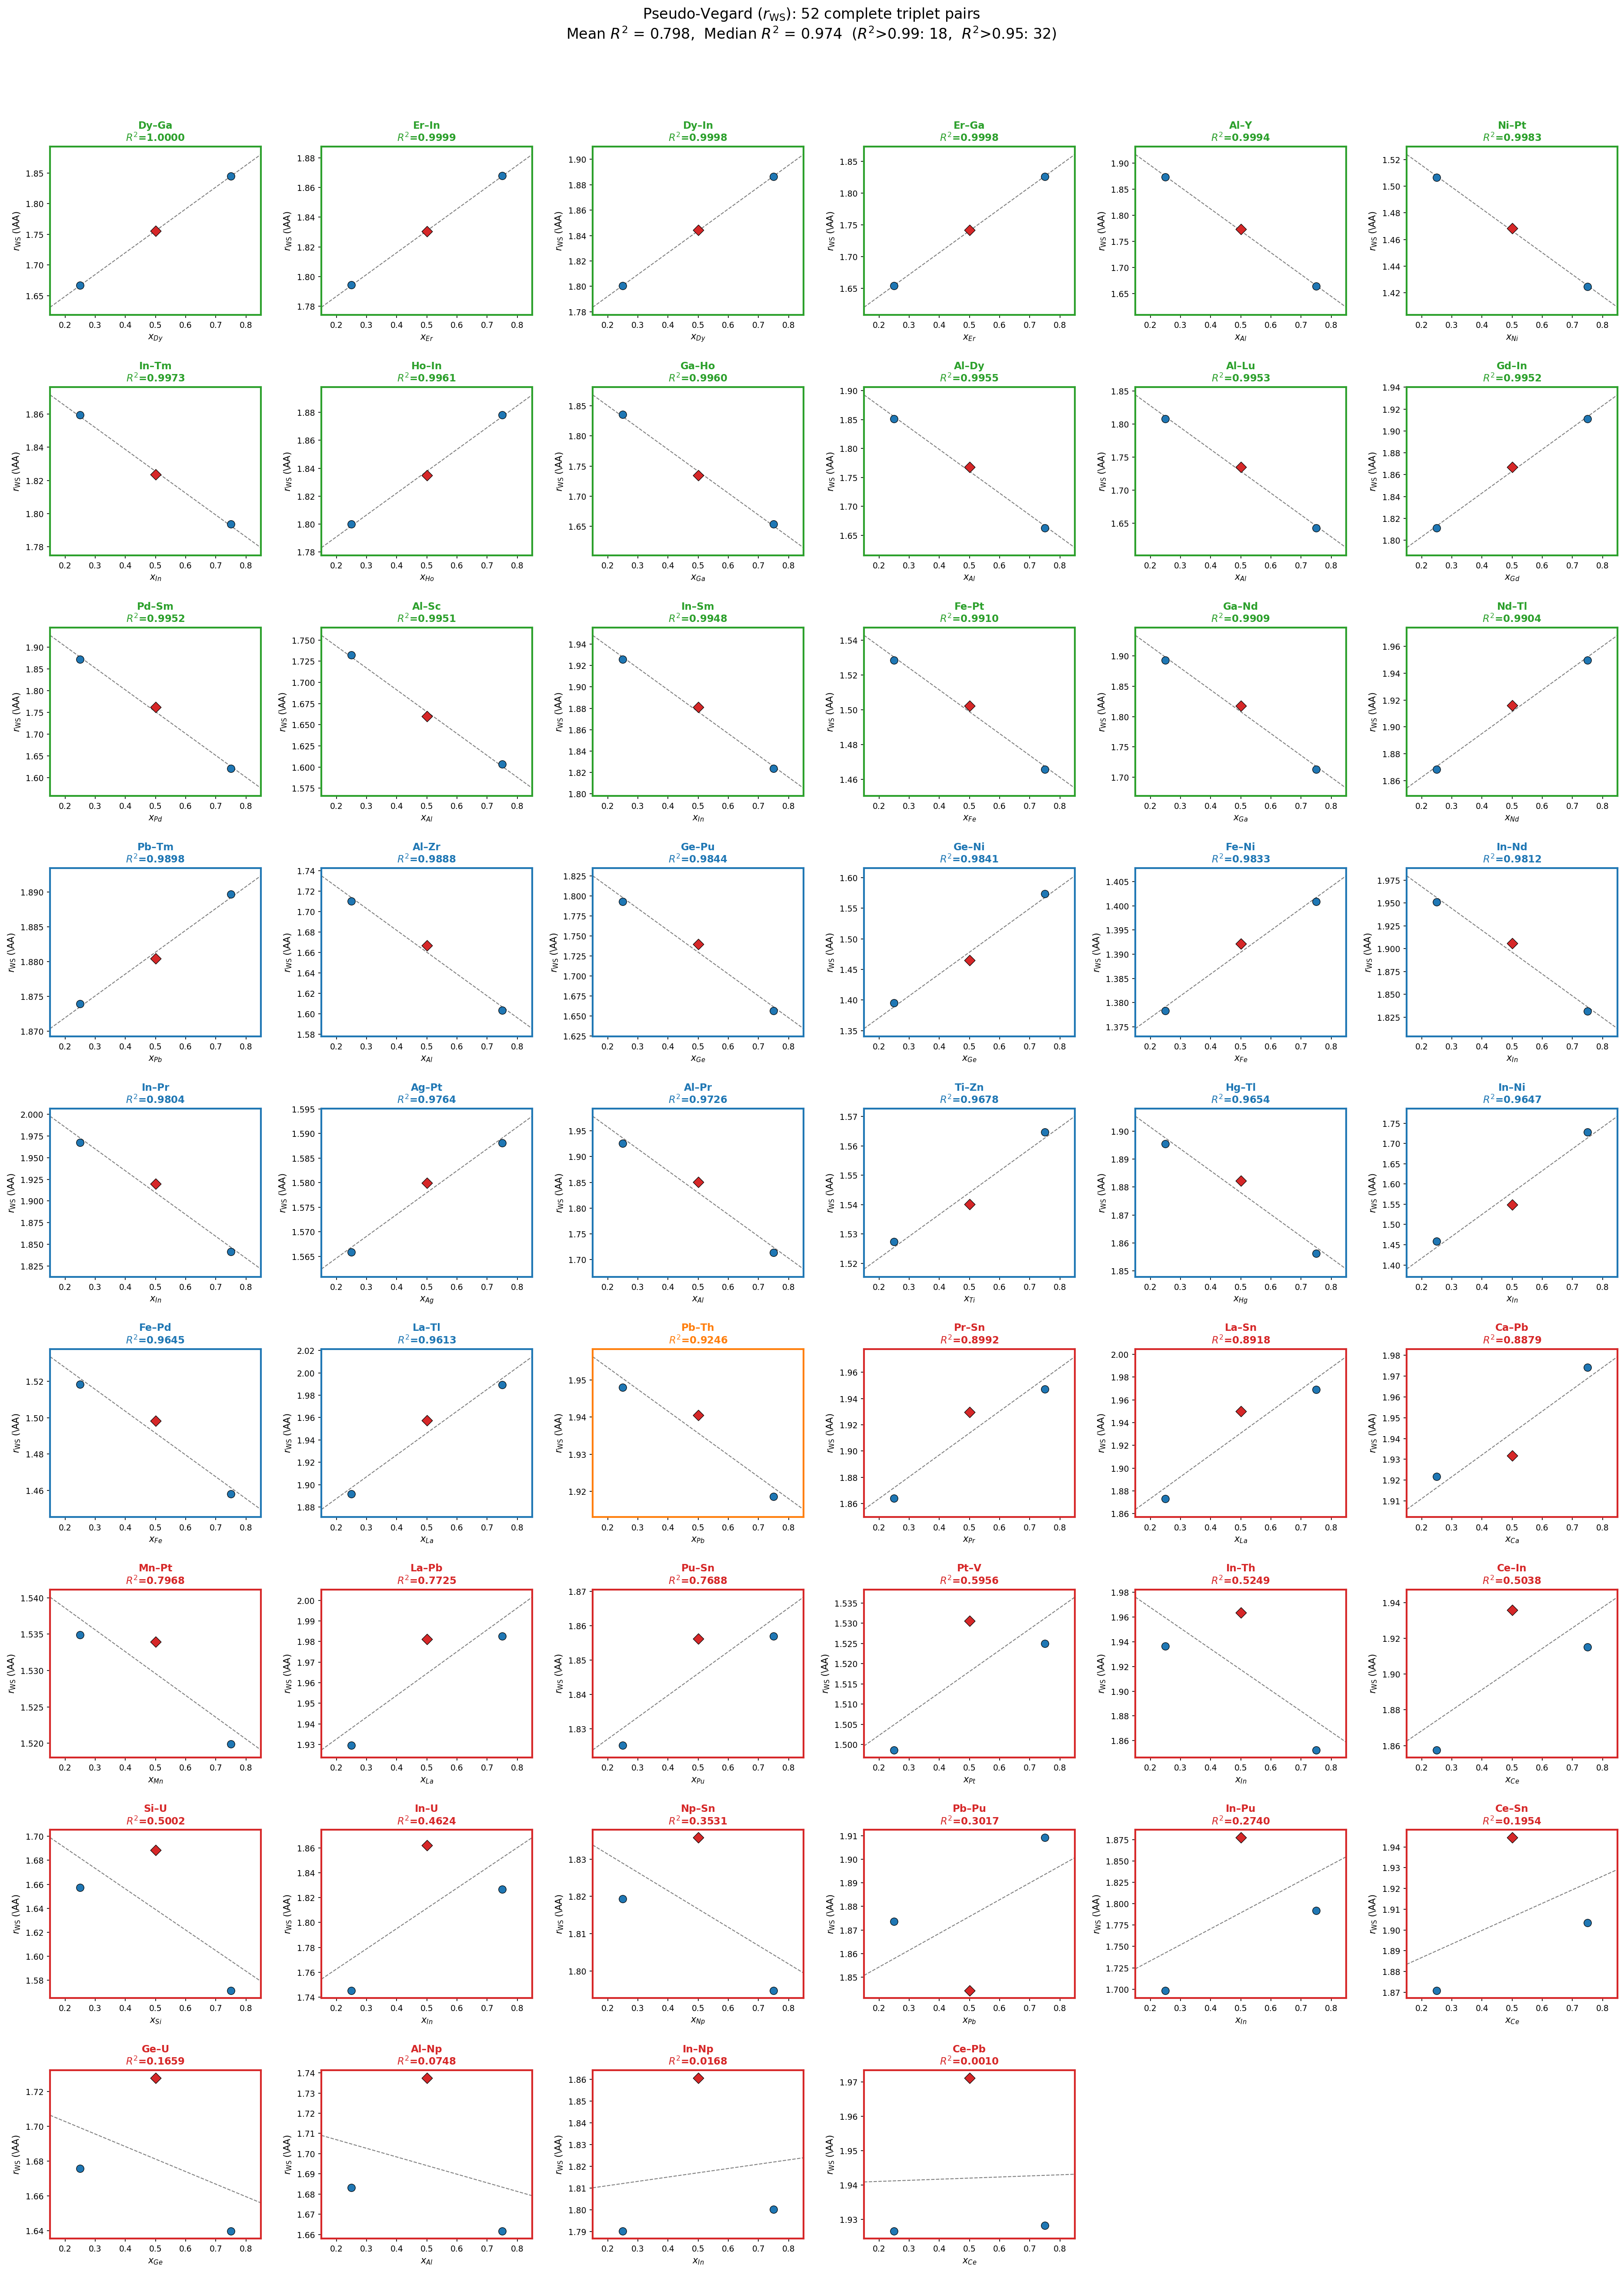
\includegraphics[width=0.95\textwidth]{vegard_triplet_summary_r_ws.png}
    \caption{3組成が揃った52ペアの$r_\mathrm{WS}$によるサマリーグリッド。$R^2$降順でソート。枠線色: 緑（$R^2 > 0.99$）、青（$>0.95$）、橙（$>0.90$）、赤（$<0.90$）。Mean $R^2 = 0.798$、Median $R^2 = 0.974$。}
    \label{fig:triplet_summary}
\end{figure*}

\subsubsection{B2偏差の解析}
L1$_2$の2点（25\%, 75\%）を結ぶ直線からB2点（50\%）がどれだけずれるかを図~\ref{fig:b2_deviation}に示す。$r_\mathrm{WS}$と$d_\mathrm{nn}$での偏差を比較すると、$r_\mathrm{WS}$での偏差が系統的に小さい。これは原子体積ベースの指標が構造差を効果的にキャンセルすることを裏付ける。

\begin{figure}[htbp]
    \centering
    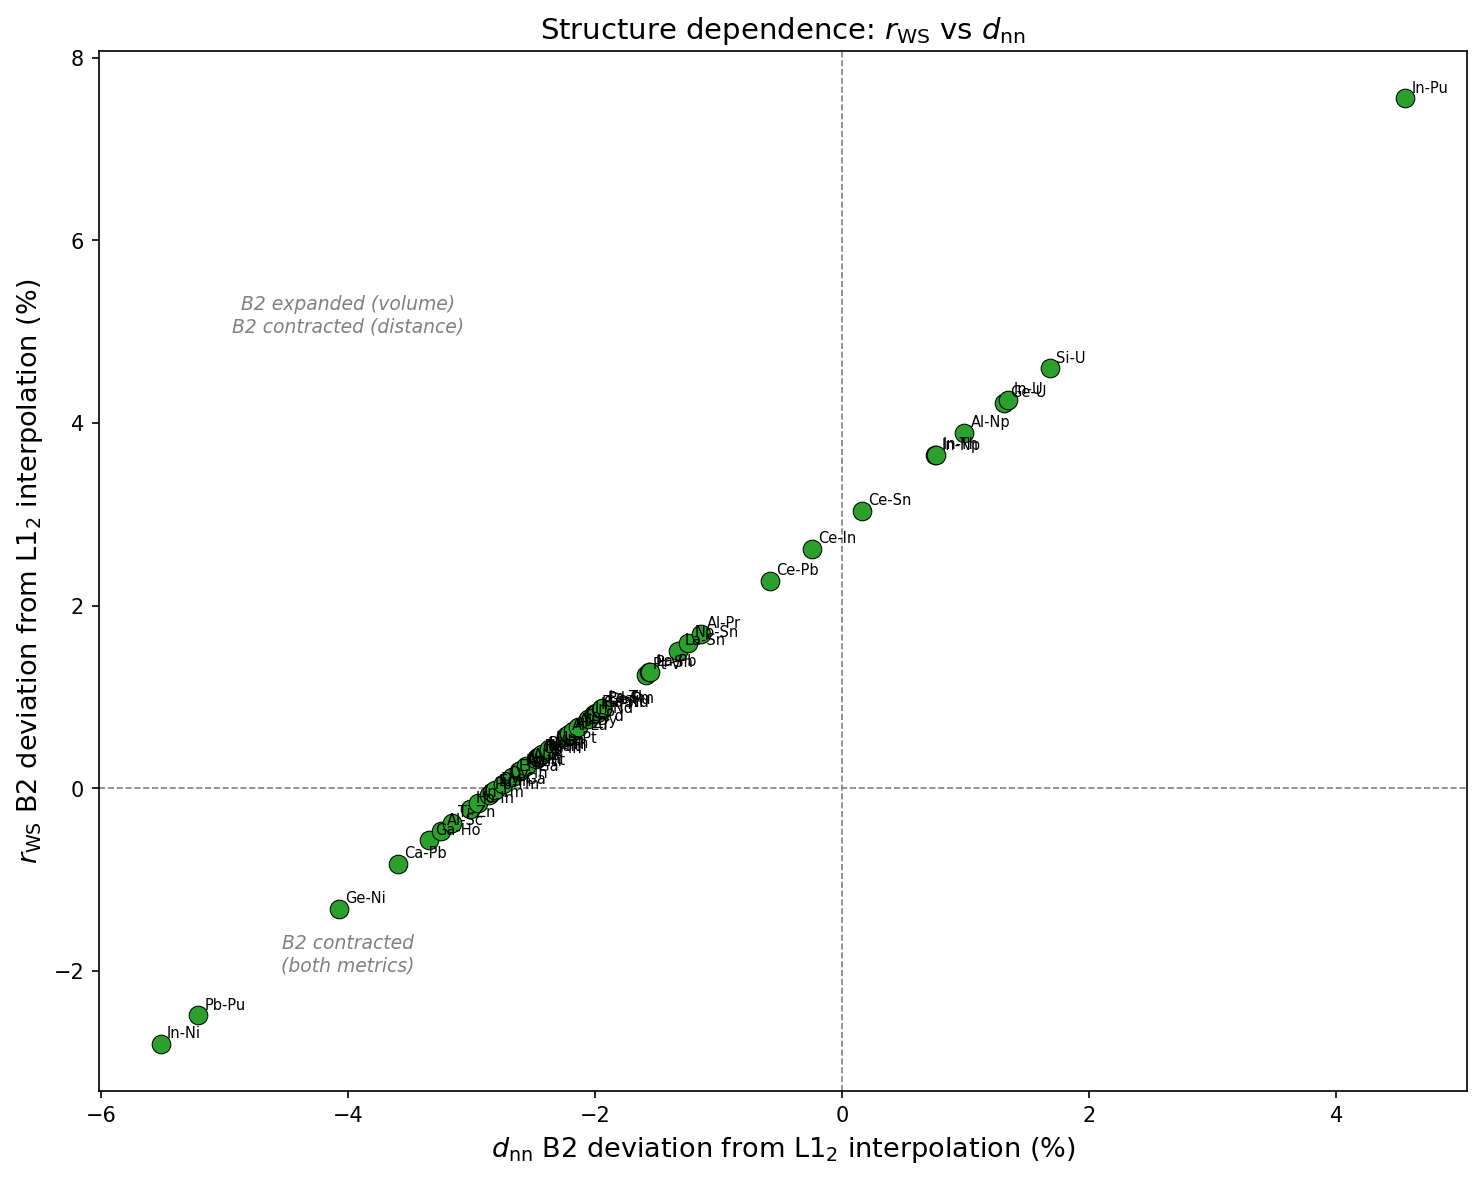
\includegraphics[width=0.45\textwidth]{vegard_rws_vs_dnn_deviation.png}
    \caption{$r_\mathrm{WS}$と$d_\mathrm{nn}$でのB2偏差の散布図。原点付近に点が集中するほど偏差が小さい。$r_\mathrm{WS}$偏差は$d_\mathrm{nn}$偏差より系統的に小さい。}
    \label{fig:b2_deviation}
\end{figure}


\subsection{Wigner--Seitz半径の包括的検証}

\subsubsection{$r_\mathrm{WS}$のBootstrap不確定性}
原子体積から求めた元素別平均$r_\mathrm{WS}$のbootstrap不確定性を表~\ref{tab:bootstrap_rws}にまとめた。1000回のリサンプリングにより算出された各元素の$r_\mathrm{WS}$標準偏差は、OQMD-B2で中央値0.018~\AA（最小）からMP-L1$_2$で0.035~\AA（最大）であった。

\begin{table*}[htbp]
\small
    \centering
    \caption{原子体積ベース$r_\mathrm{WS}$のBootstrap不確定性（1000回リサンプリング）。}
    \label{tab:bootstrap_rws}
    \begin{tabular}{lccccc}
        \toprule
        ケース & 元素数 & 中央値 std (\AA) & 最大 std (\AA) & 平均 95\% CI (\AA) & 最大 std 元素 \\
        \midrule
        MP-B2 & 68 & 0.021 & 0.079 & 0.092 & Si \\
        MP-L1$_2$ & 72 & 0.035 & 0.209 & 0.156 & Re \\
        OQMD-B2 & 72 & 0.018 & 0.027 & 0.073 & Li \\
        OQMD-L1$_2$ & 58 & 0.030 & 0.066 & 0.113 & Eu \\
        \bottomrule
    \end{tabular}
\end{table*}

図~\ref{fig:bootstrap_rws}にMP-B2の場合のbootstrap結果を示す。各元素について$r_\mathrm{WS}$の平均値と95\%信頼区間をエラーバーで表示している。

\begin{figure}[htbp]
    \centering
    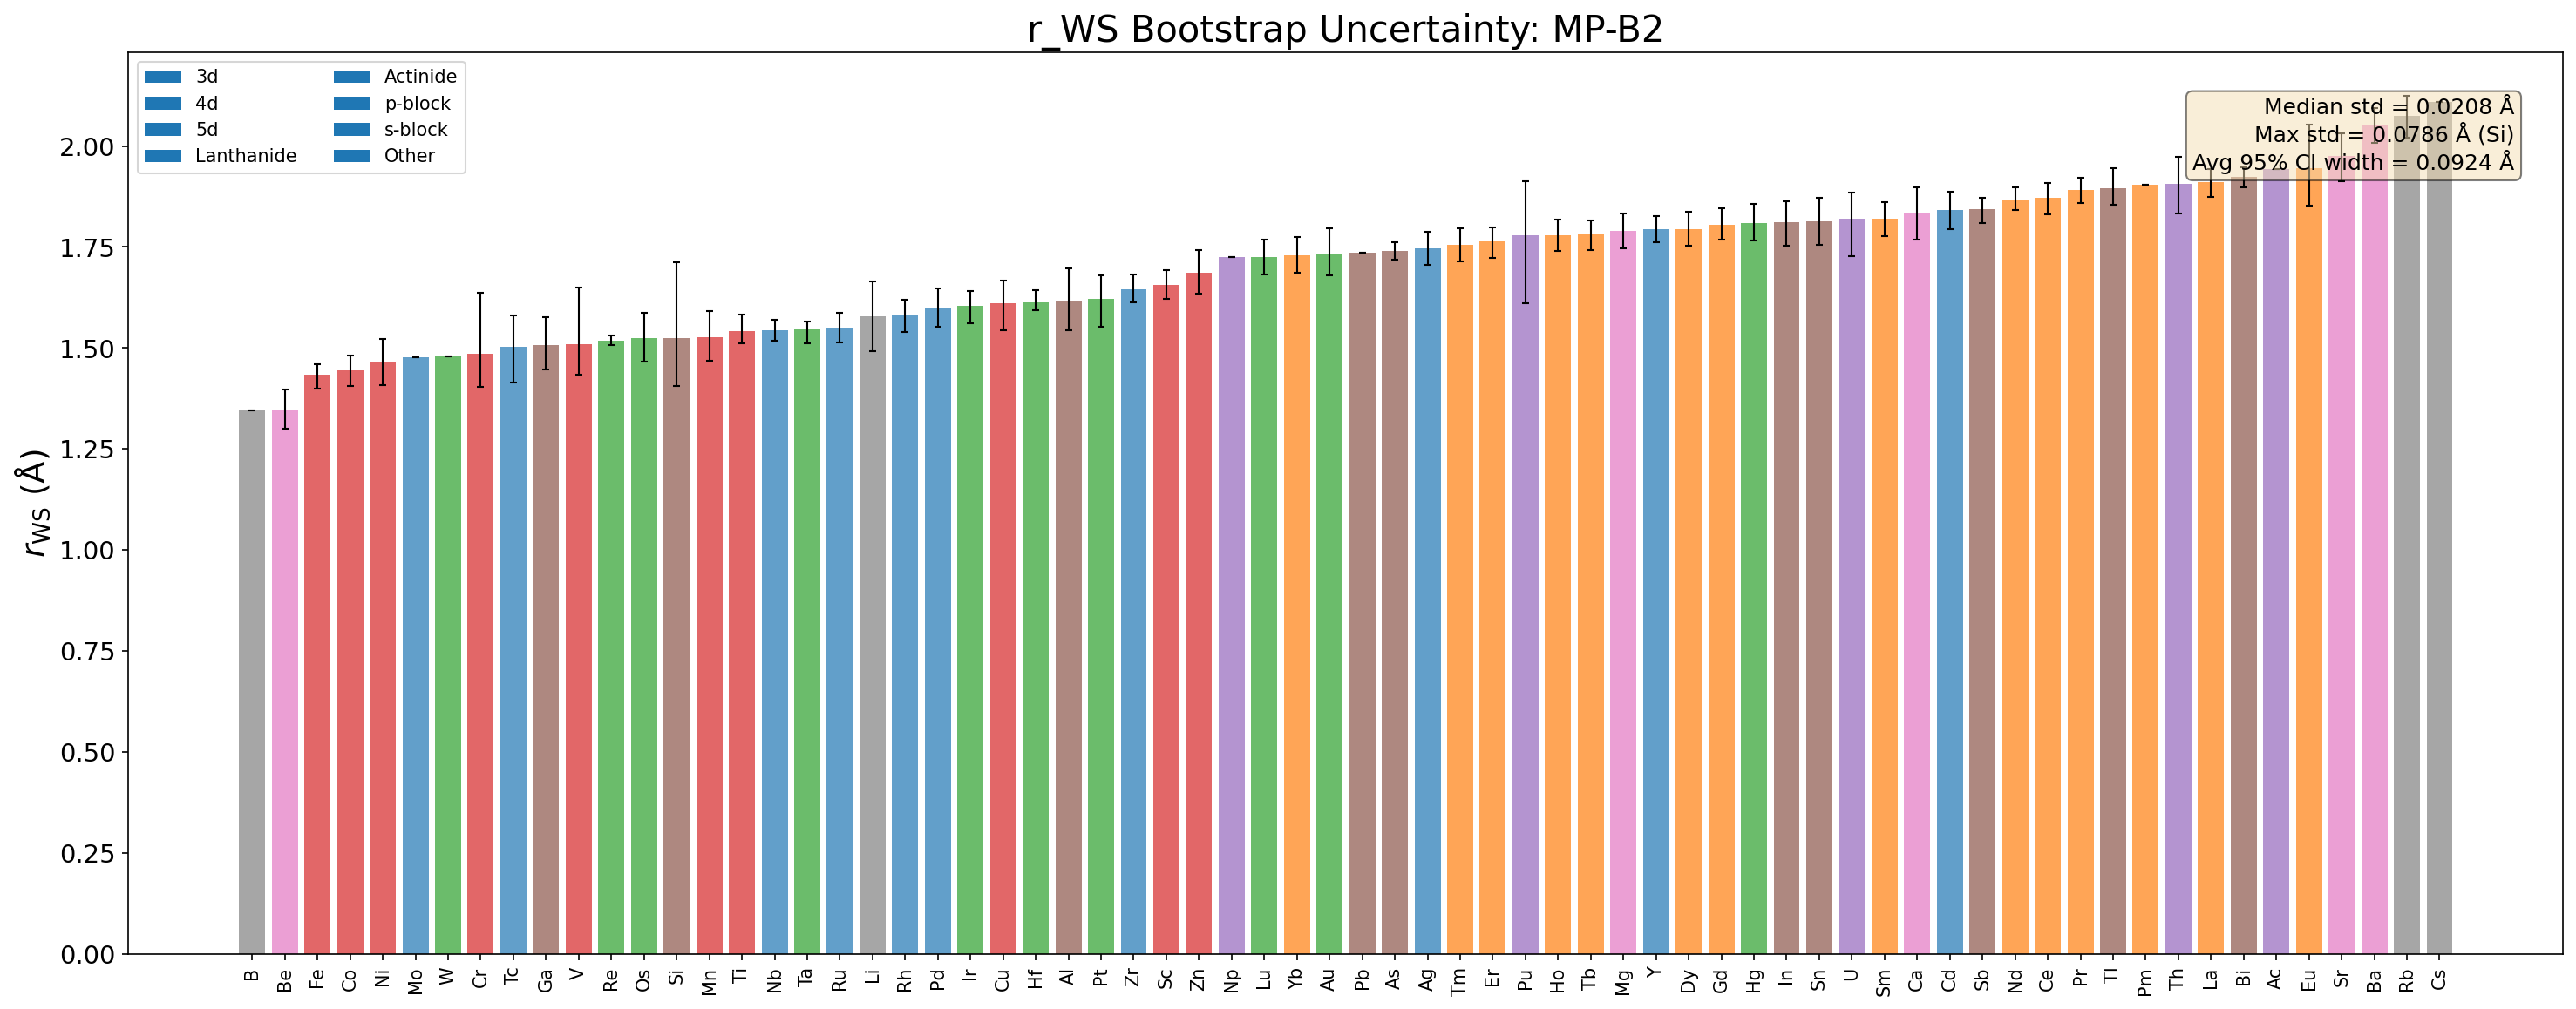
\includegraphics[width=0.45\textwidth]{bootstrap_rws_MP_B2.png}
    \caption{MP-B2の元素別$r_\mathrm{WS}$のbootstrap結果（1000回リサンプリング）。エラーバーは95\%信頼区間。中央値 std = 0.021~\AA。}
    \label{fig:bootstrap_rws}
\end{figure}


\subsubsection{$r_\mathrm{WS}$と有効接触半径の比較}
正しいWigner--Seitz半径の定義（式~\ref{eq:r_ws}）により、$r_\mathrm{WS}$の値は1.378--1.989~\AA となり、最適化接触半径（1.2--2.0~\AA）と同スケールである。各元素について、DFT格子定数から算出した平均$r_\mathrm{WS}$と最適化接触半径$r_\mathrm{contact}$の比率を分析した結果を表~\ref{tab:rws_vs_contact}に示す。

\begin{table*}[htbp]
\small
    \centering
    \caption{$r_\mathrm{WS}$と有効接触半径の比較。$r_\mathrm{contact}/r_\mathrm{WS}$比の統計を示す。}
    \label{tab:rws_vs_contact}
    \begin{tabular}{lcccccc}
        \toprule
        ケース & 化合物数 & 元素数 & $r_\mathrm{contact}/r_\mathrm{WS}$ 平均 & std & 最小 & 最大 \\
        \midrule
        MP-B2 & 357 & 68 & 0.900 & 0.069 & 0.781 & 1.016 \\
        MP-L1$_2$ & 848 & 72 & 0.859 & 0.087 & 0.305 & 0.973 \\
        OQMD-B2 & 2539 & 72 & 0.872 & 0.068 & 0.714 & 1.015 \\
        OQMD-L1$_2$ & 238 & 58 & 0.905 & 0.069 & 0.643 & 1.167 \\
        \bottomrule
    \end{tabular}
\end{table*}

$r_\mathrm{contact}/r_\mathrm{WS}$比は全ケースで平均0.86--0.91の範囲にあり、接触半径は$r_\mathrm{WS}$の約85--91\%に相当する。これは、max基準モデルの接触半径が剛体球の重なりを避ける最小距離から定まるため、$r_\mathrm{WS}$（原子体積保存球）よりも系統的に小さくなるという物理的に合理的な結果である。

図~\ref{fig:rws_vs_contact}に元素別の$r_\mathrm{WS}$ vs $r_\mathrm{contact}$のパリティプロットを示す。トレンドから外れるアウトライヤーには元素名ラベルが付与されている。

\begin{figure*}[t]
  \centering
  \begin{minipage}[t]{0.48\textwidth}
    \centering
    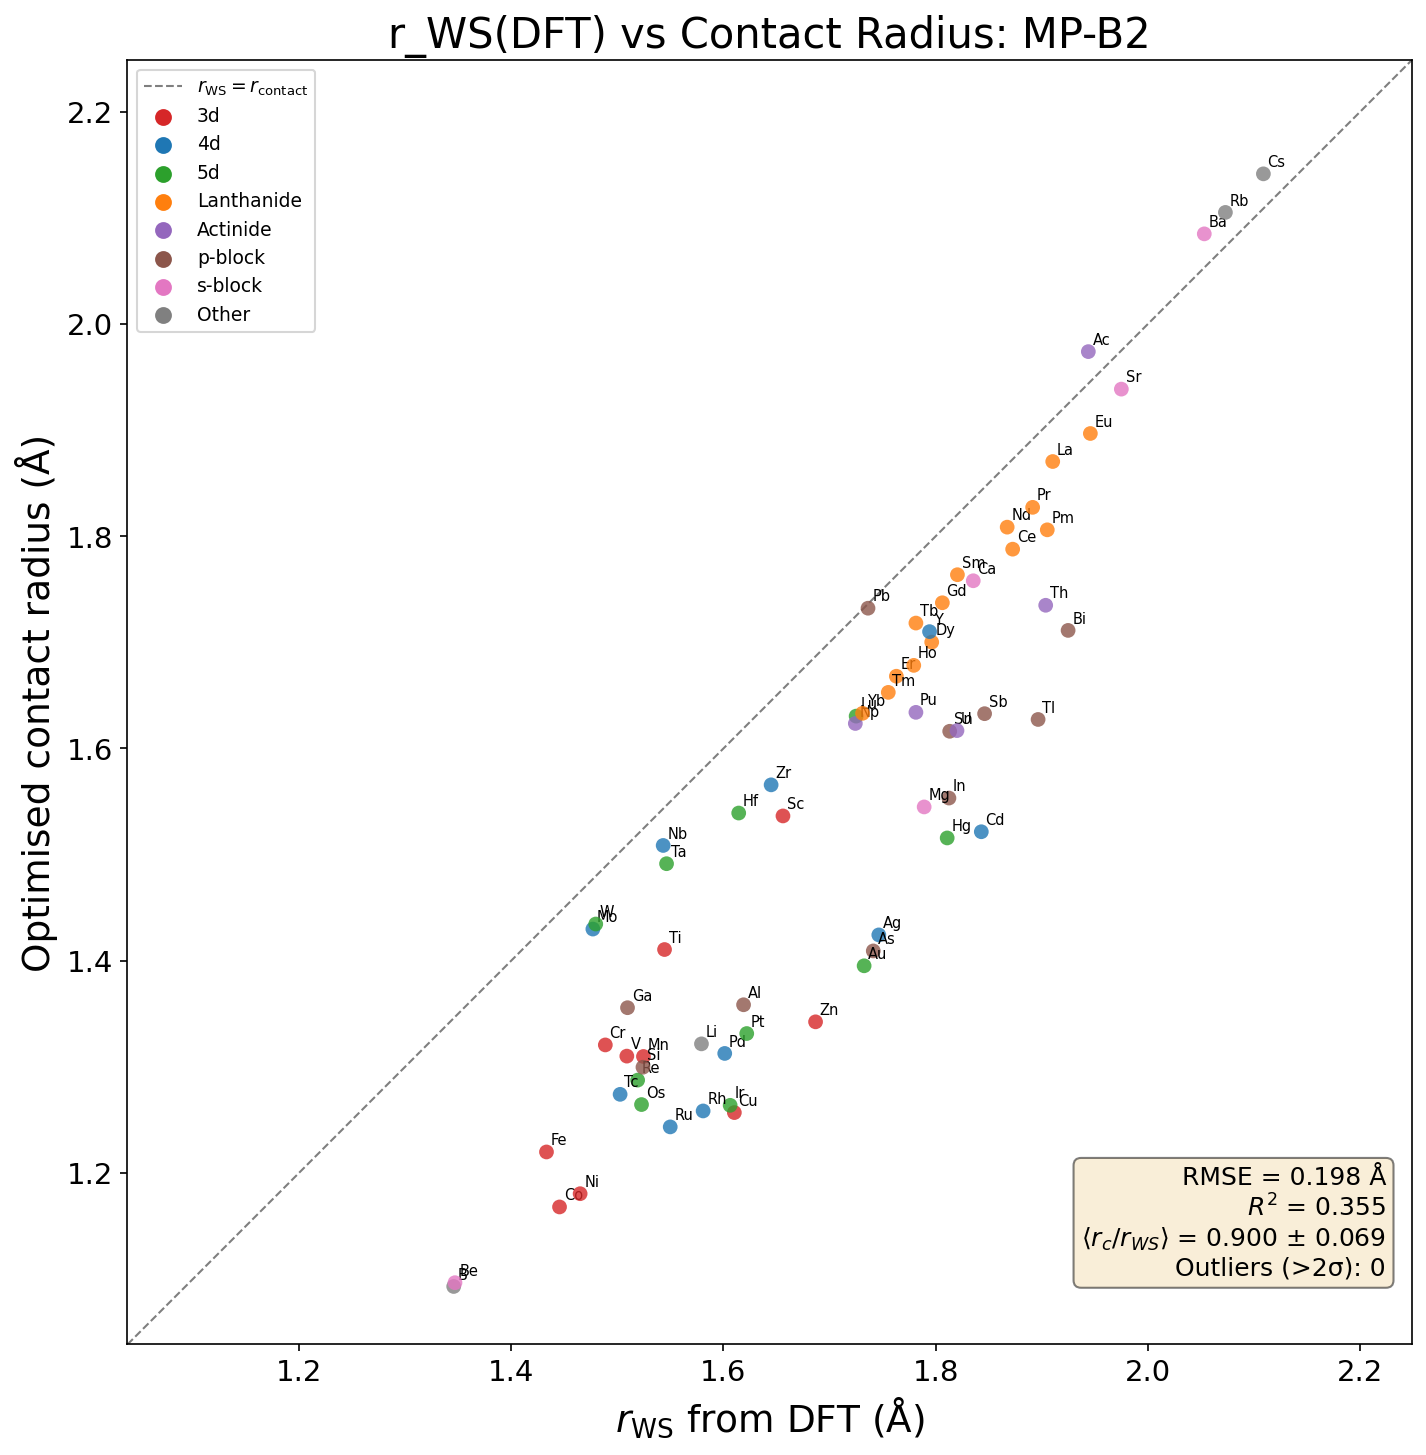
\includegraphics[width=0.95\linewidth]{rws_vs_contact_MP_B2.png}
    \caption{MP-B2: $r_\mathrm{WS}$ vs 接触半径。赤太字ラベルはトレンドから$>2\sigma$逸脱するアウトライヤー。}
    \label{fig:rws_contact_mp_b2}
  \end{minipage}
  \hfill
  \begin{minipage}[t]{0.48\textwidth}
    \centering
    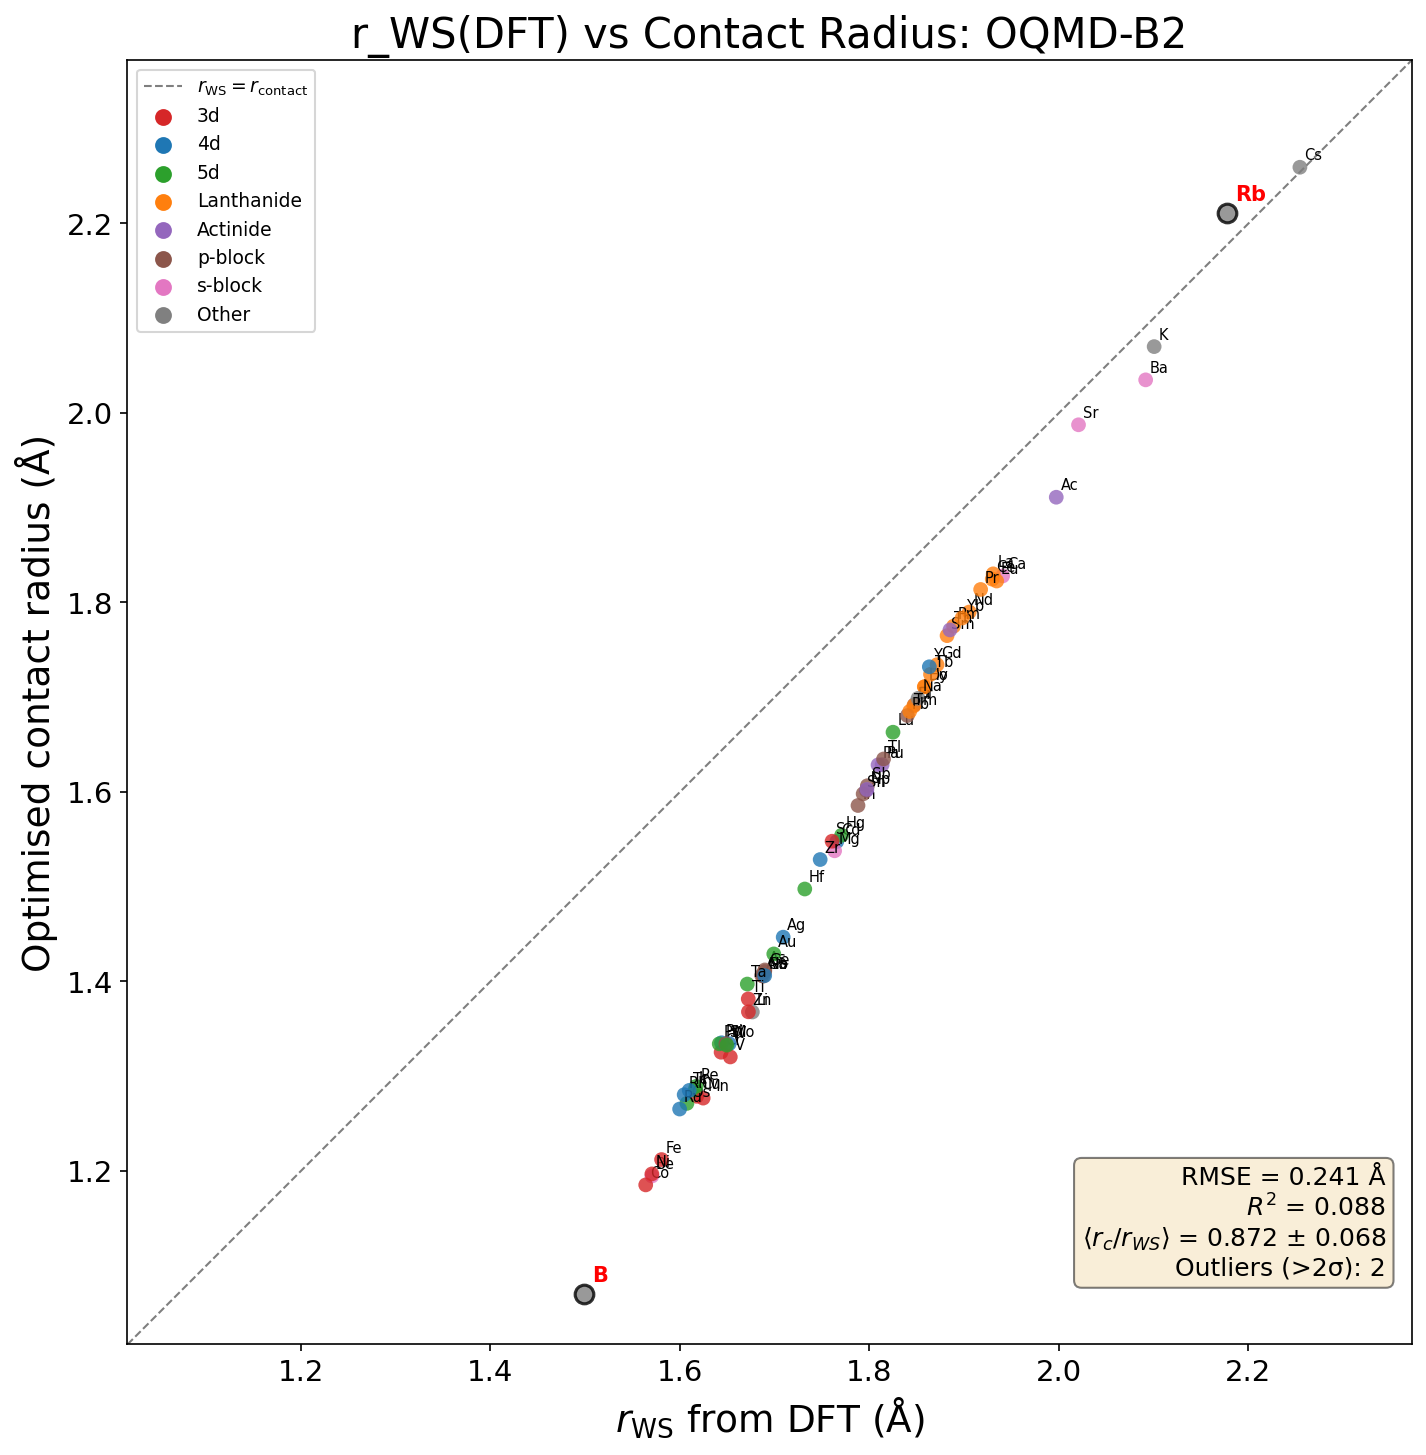
\includegraphics[width=0.95\linewidth]{rws_vs_contact_OQMD_B2.png}
    \caption{OQMD-B2: $r_\mathrm{WS}$ vs 接触半径。同様にアウトライヤーをラベル表示。}
    \label{fig:rws_contact_oqmd_b2}
  \end{minipage}
\end{figure*}

\begin{figure*}[t]
  \centering
  \begin{minipage}[t]{0.48\textwidth}
    \centering
    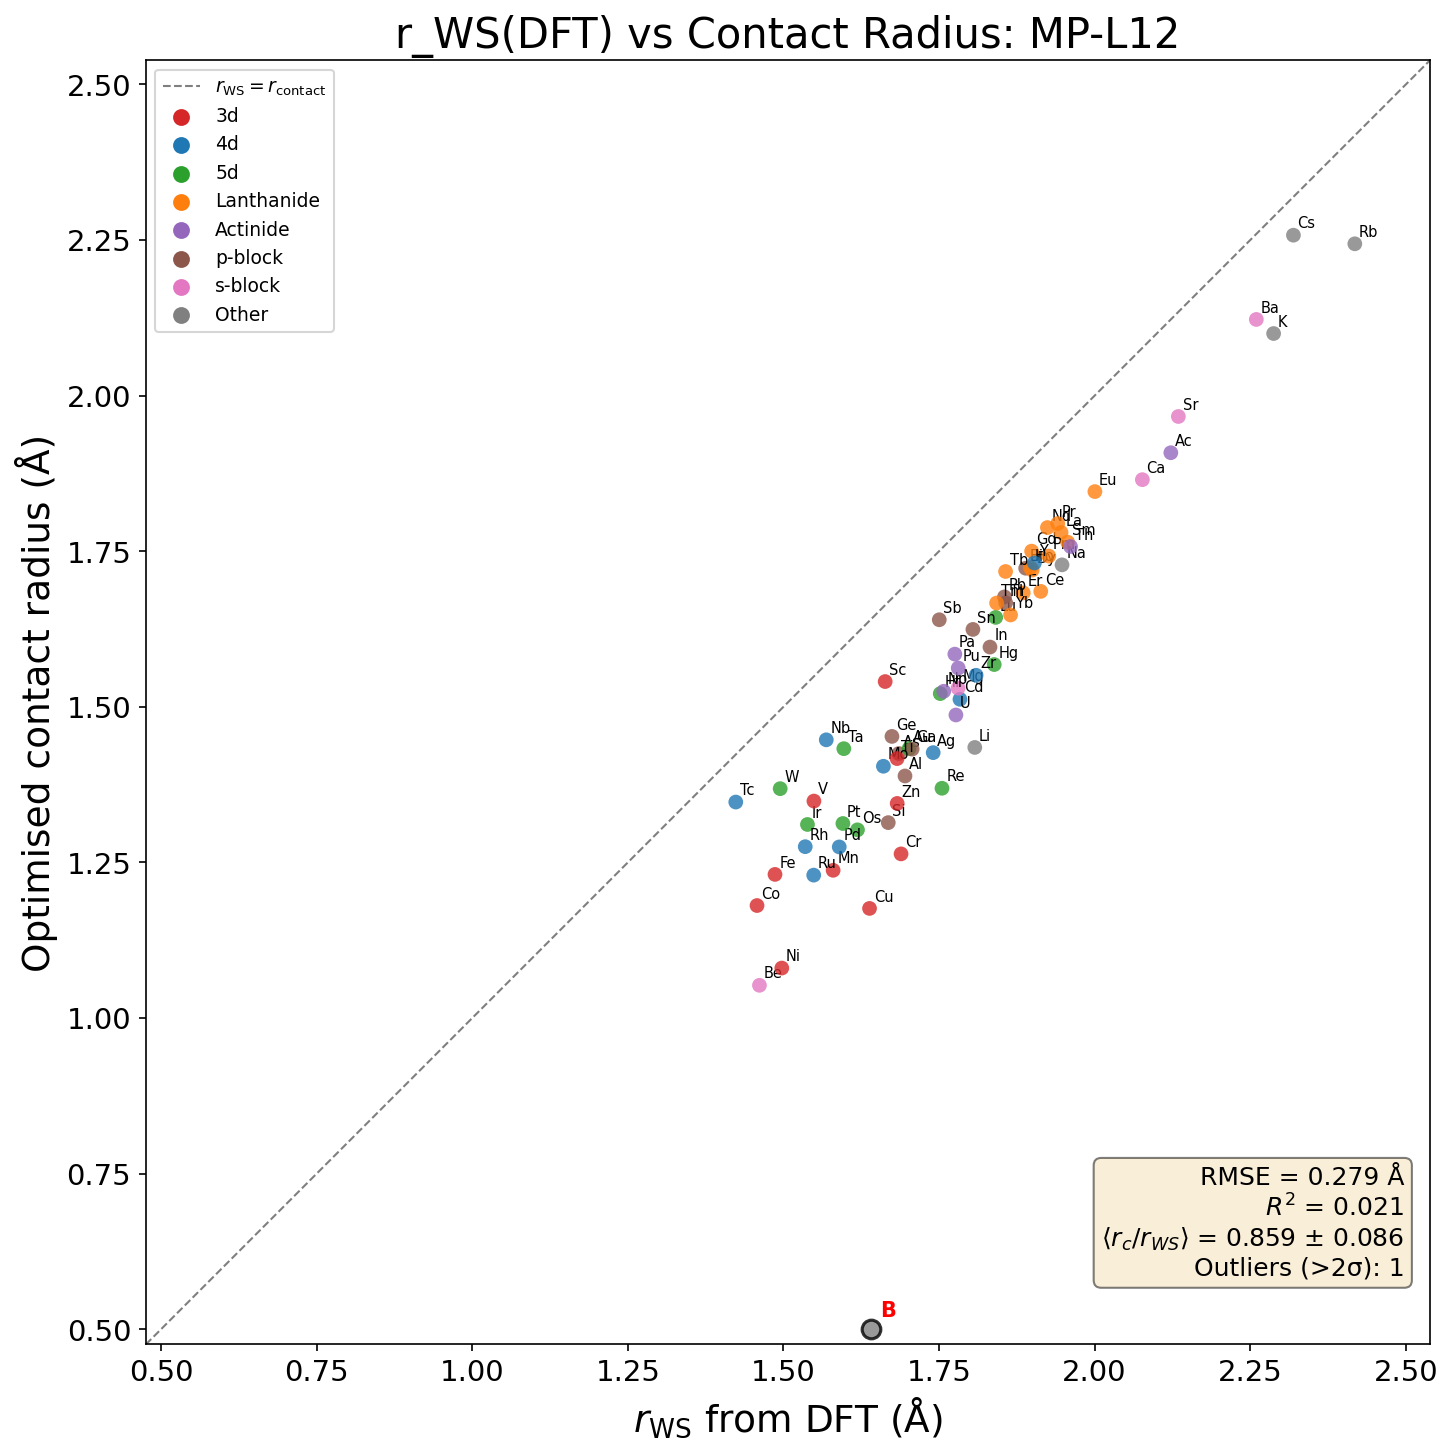
\includegraphics[width=0.95\linewidth]{rws_vs_contact_MP_L12.png}
    \caption{MP-L1$_2$: $r_\mathrm{WS}$ vs 接触半径。L1$_2$ではCase 1/2の接触条件切替により散らばりが大きい。}
    \label{fig:rws_contact_mp_l12}
  \end{minipage}
  \hfill
  \begin{minipage}[t]{0.48\textwidth}
    \centering
    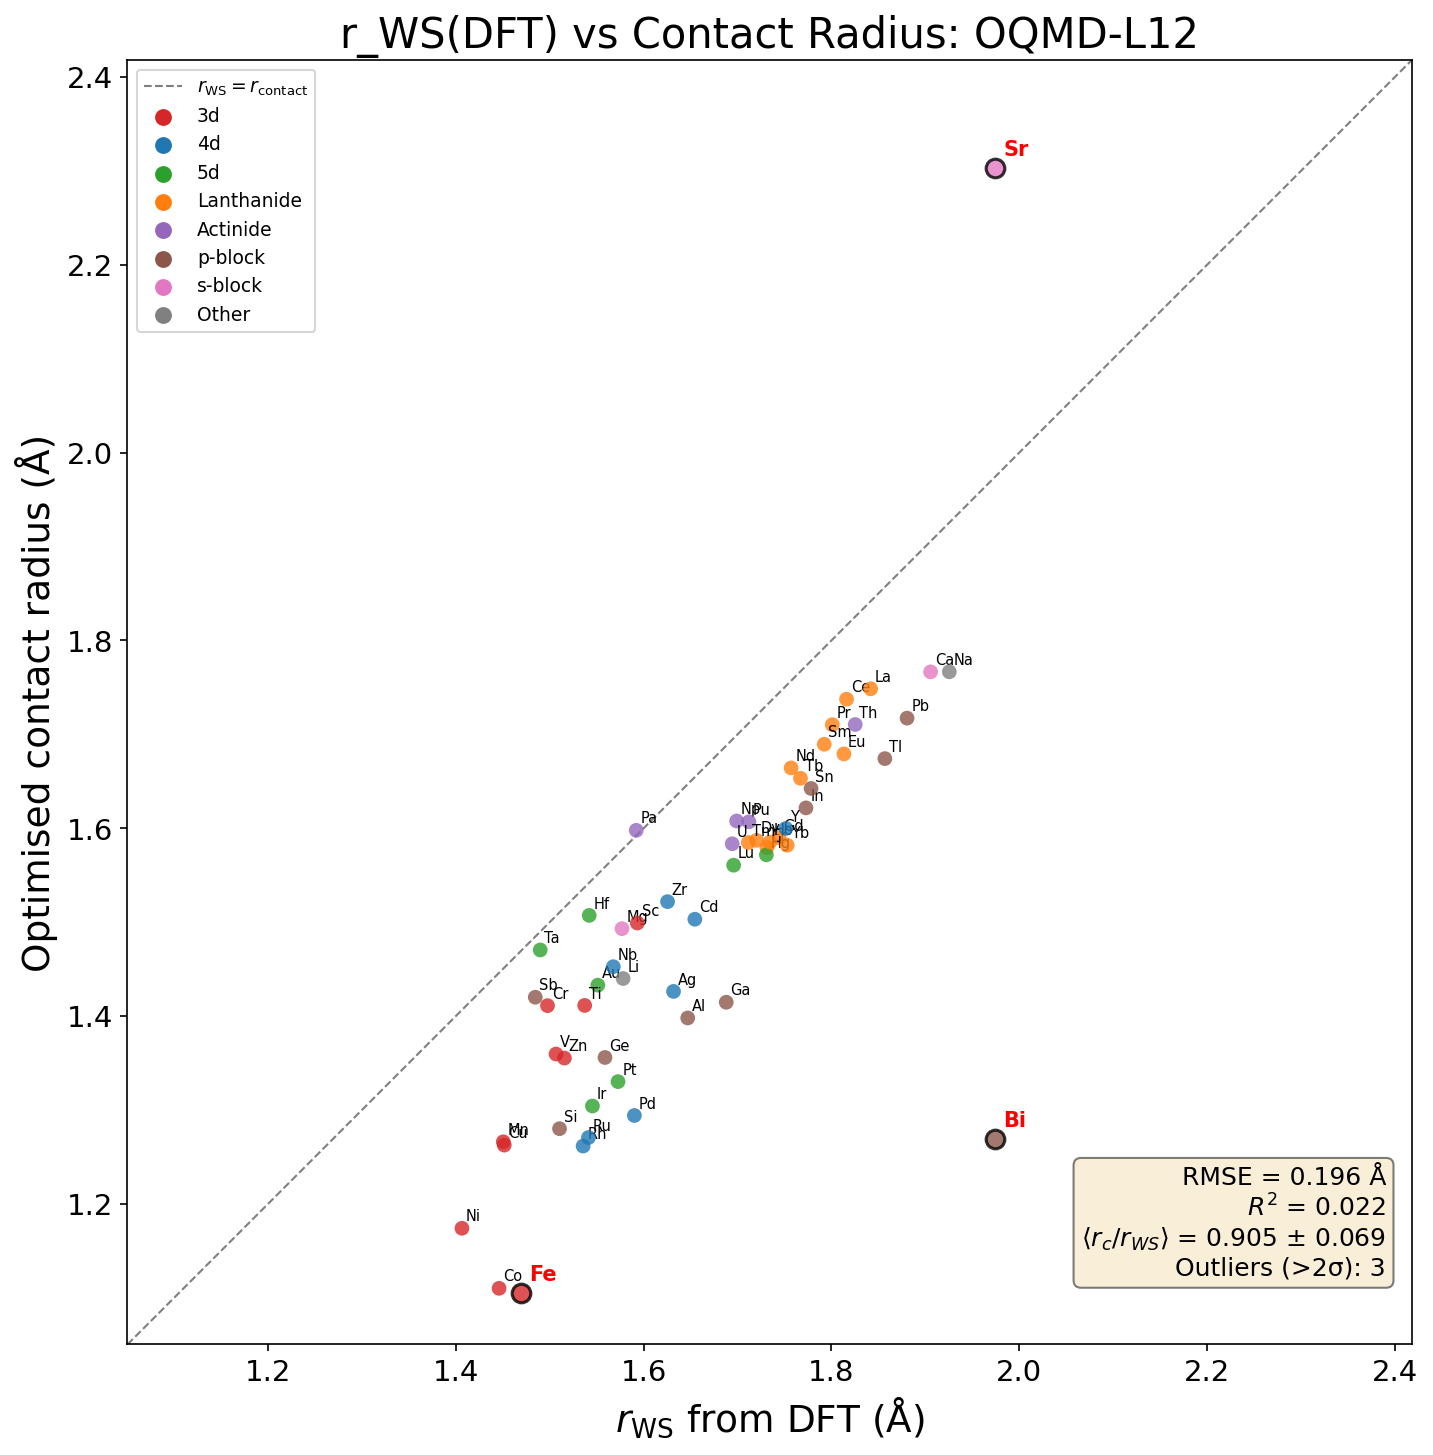
\includegraphics[width=0.95\linewidth]{rws_vs_contact_OQMD_L12.png}
    \caption{OQMD-L1$_2$: $r_\mathrm{WS}$ vs 接触半径。$r_\mathrm{contact}/r_\mathrm{WS}$ 平均 = 0.905。}
    \label{fig:rws_contact_oqmd_l12}
  \end{minipage}
\end{figure*}


\subsubsection{化合物レベルの$r_\mathrm{WS}$パリティ}
DFT格子定数から算出した$r_\mathrm{WS}$(DFT)と、最適化半径から予測した$r_\mathrm{WS}$(pred)の化合物レベルのパリティプロットを図~\ref{fig:compound_parity}に示す。アウトライヤーには化合物名がラベル表示されている。

\begin{figure*}[t]
  \centering
  \begin{minipage}[t]{0.48\textwidth}
    \centering
    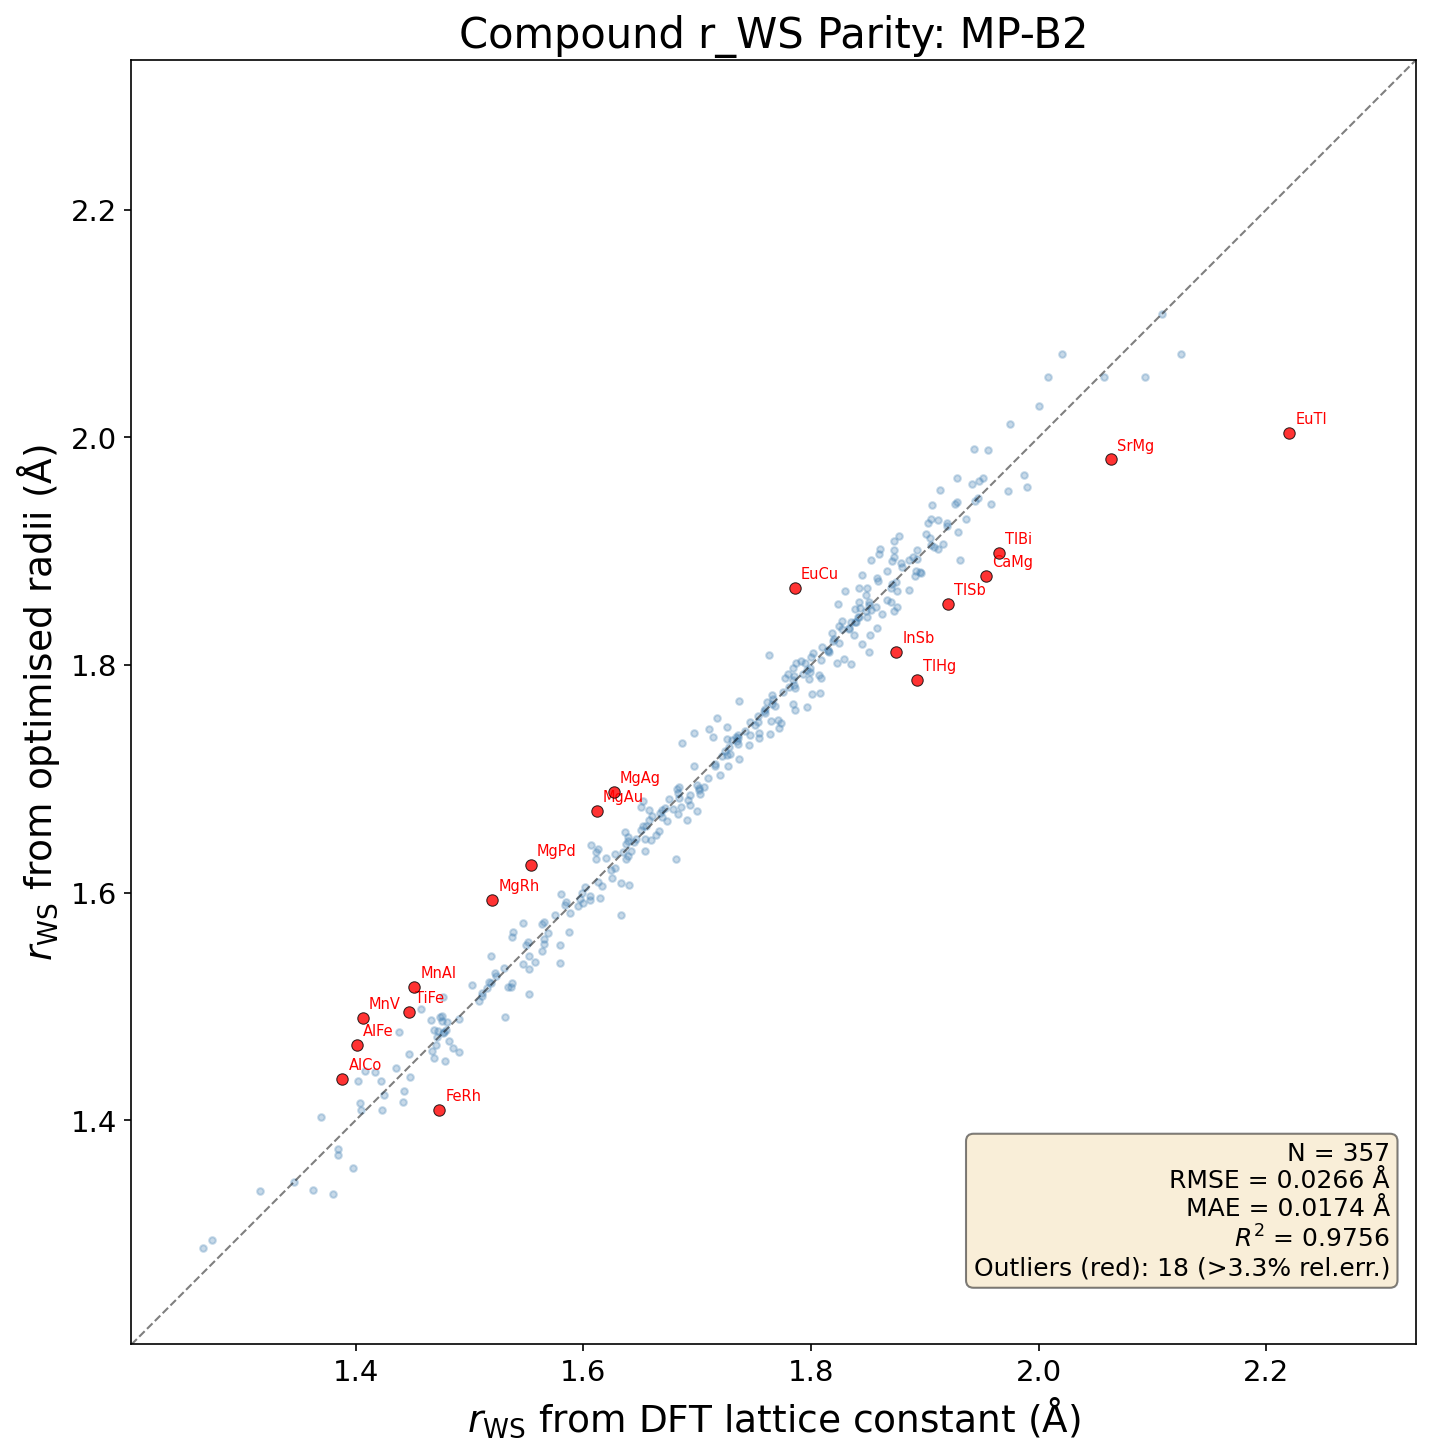
\includegraphics[width=0.95\linewidth]{compound_rws_parity_MP_B2.png}
    \caption{MP-B2: 化合物レベル$r_\mathrm{WS}$パリティ。RMSE = 0.027~\AA、$R^2 = 0.976$。赤ラベルはアウトライヤー化合物。}
    \label{fig:compound_parity_mp_b2}
  \end{minipage}
  \hfill
  \begin{minipage}[t]{0.48\textwidth}
    \centering
    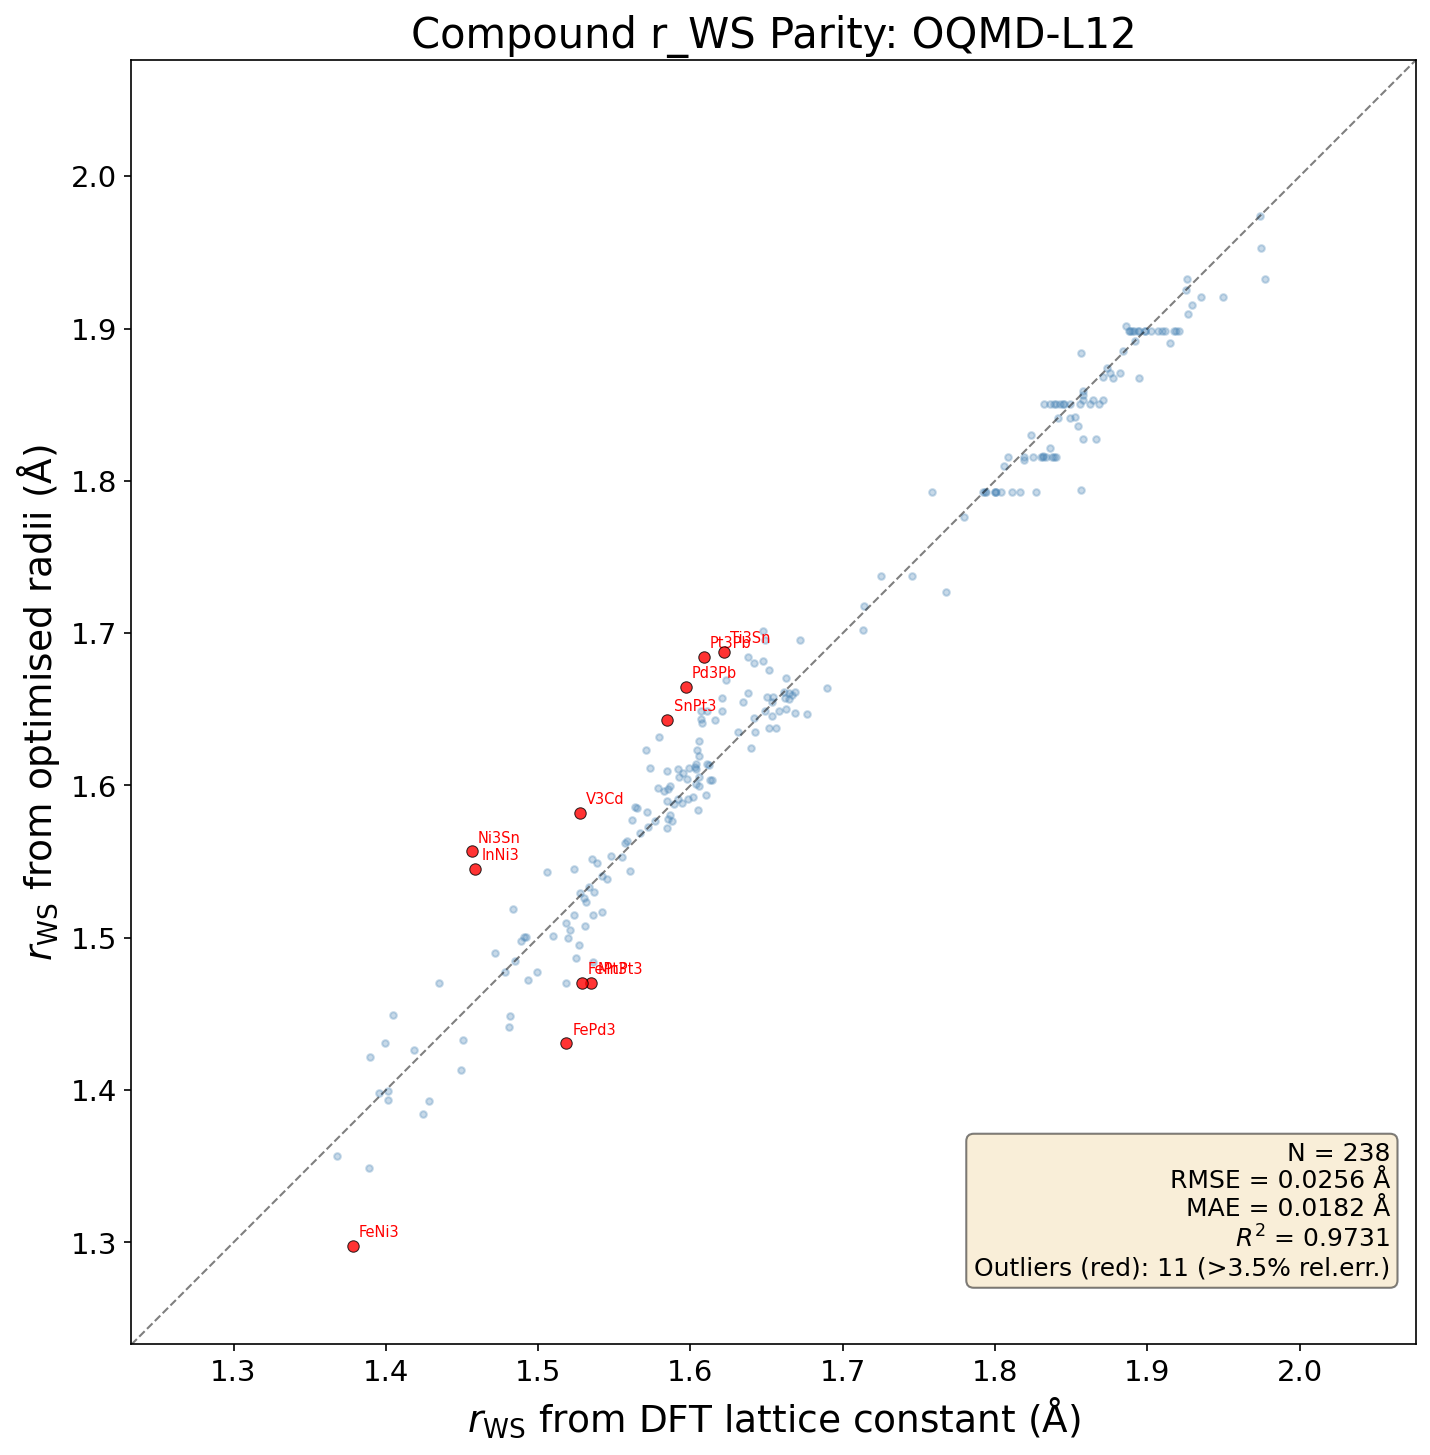
\includegraphics[width=0.95\linewidth]{compound_rws_parity_OQMD_L12.png}
    \caption{OQMD-L1$_2$: 化合物レベル$r_\mathrm{WS}$パリティ。RMSE = 0.026~\AA、$R^2 = 0.973$。}
    \label{fig:compound_parity_oqmd_l12}
  \end{minipage}
\end{figure*}

\begin{figure*}[t]
  \centering
  \begin{minipage}[t]{0.48\textwidth}
    \centering
    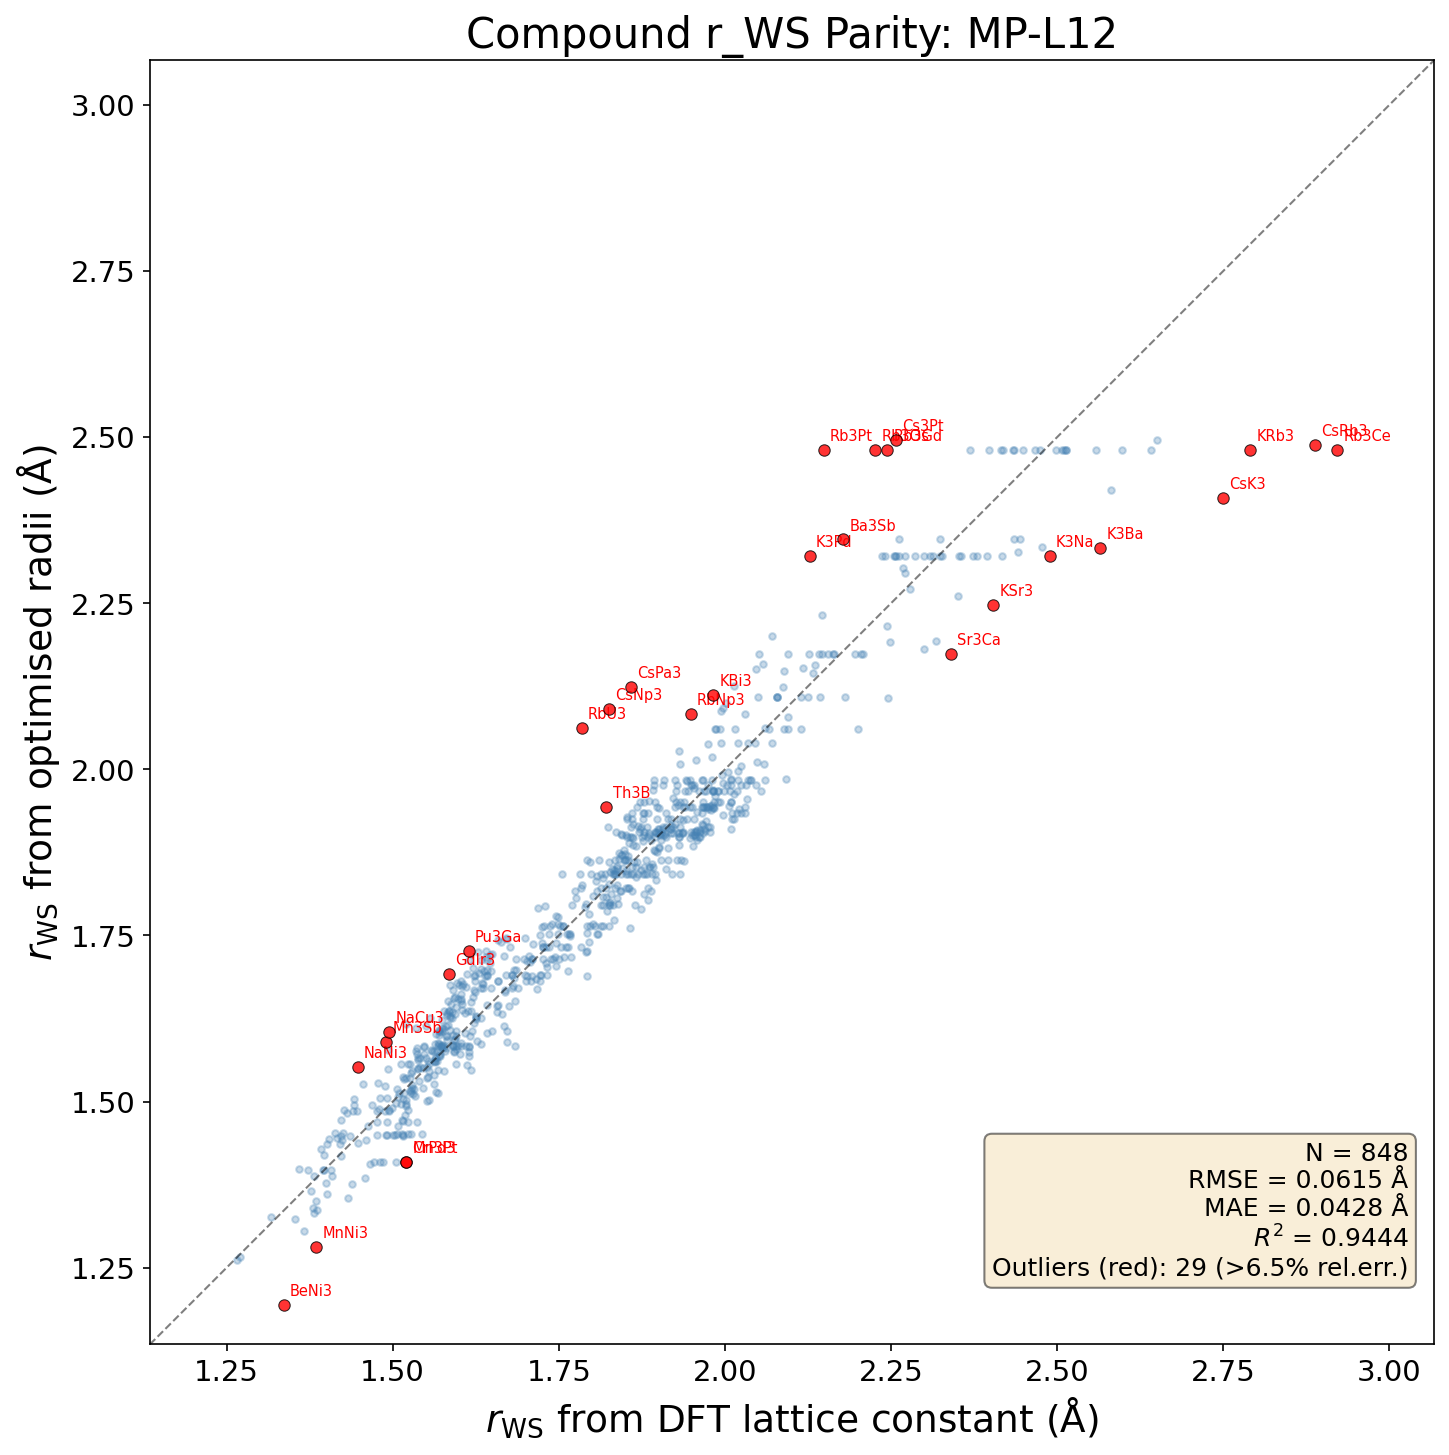
\includegraphics[width=0.95\linewidth]{compound_rws_parity_MP_L12.png}
    \caption{MP-L1$_2$: 化合物レベル$r_\mathrm{WS}$パリティ。RMSE = 0.062~\AA、$R^2 = 0.944$。}
    \label{fig:compound_parity_mp_l12}
  \end{minipage}
  \hfill
  \begin{minipage}[t]{0.48\textwidth}
    \centering
    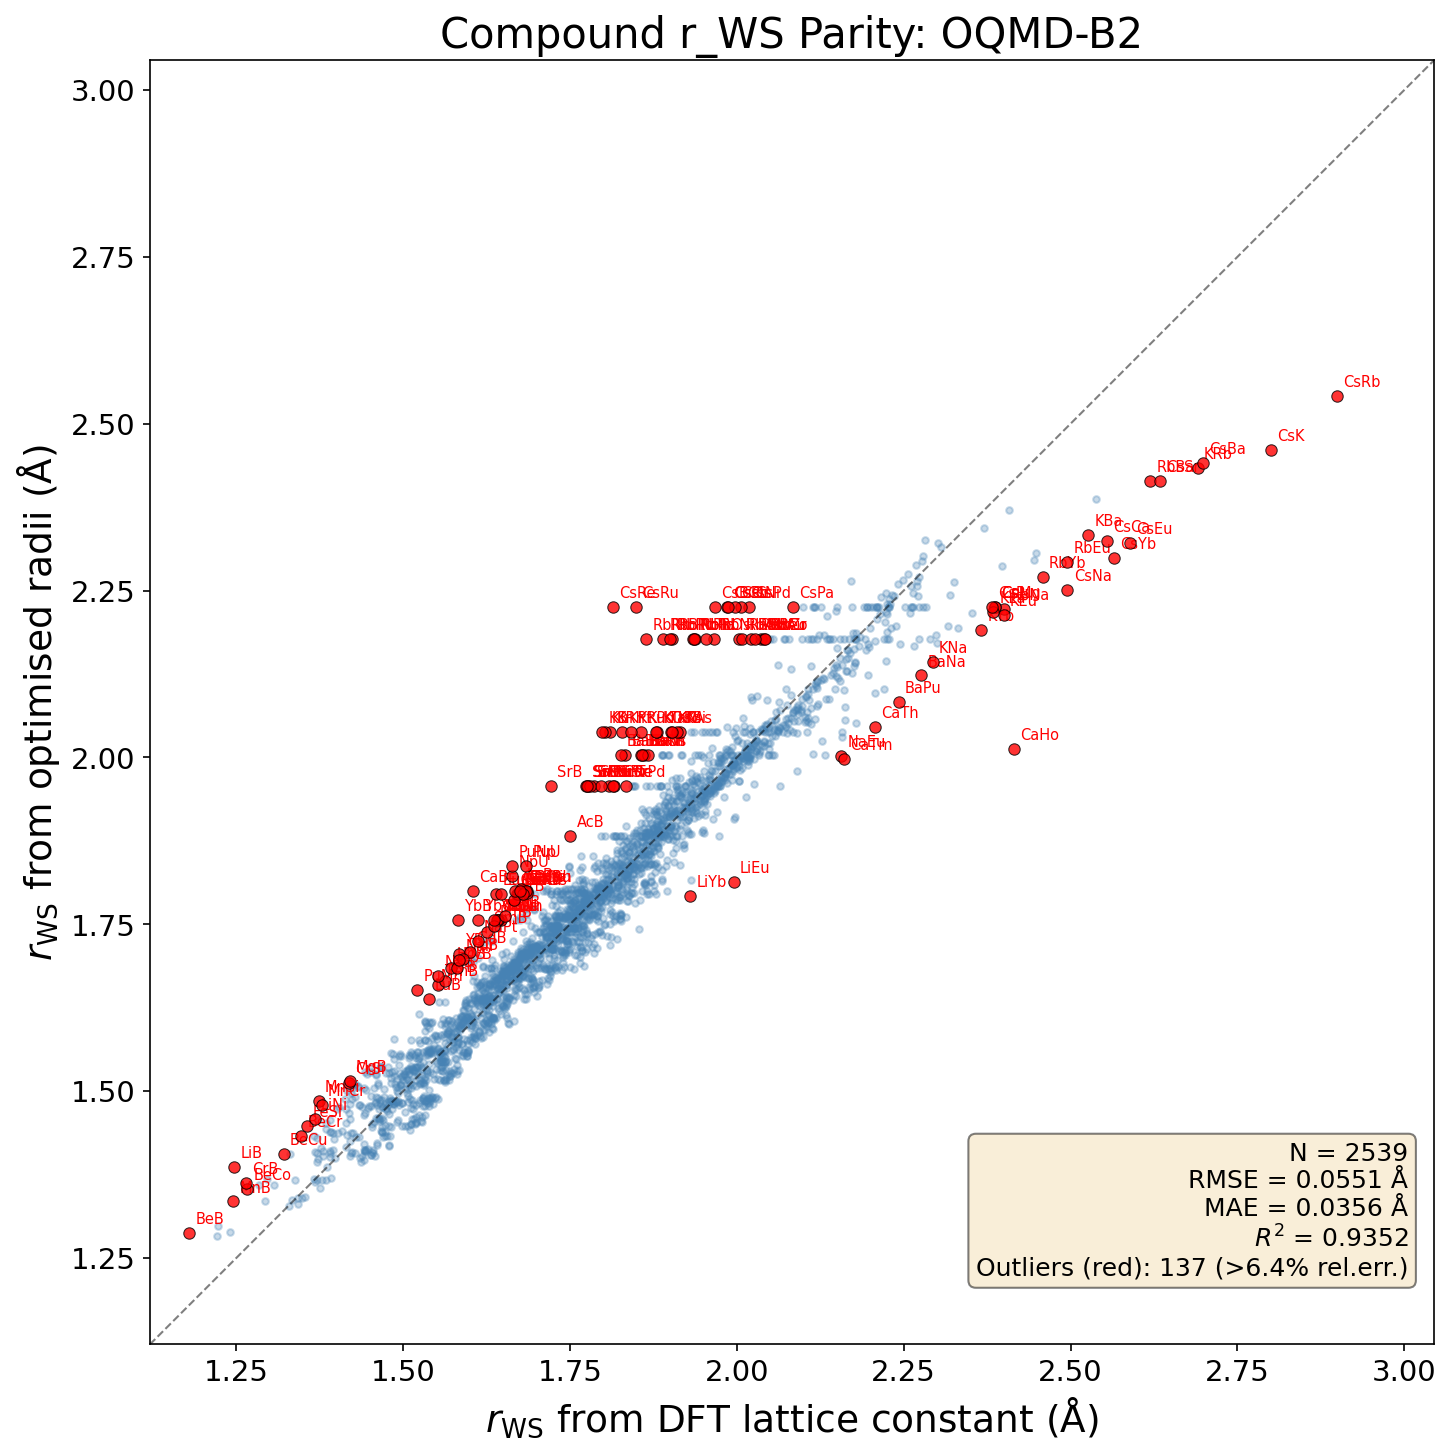
\includegraphics[width=0.95\linewidth]{compound_rws_parity_OQMD_B2.png}
    \caption{OQMD-B2: 化合物レベル$r_\mathrm{WS}$パリティ。RMSE = 0.055~\AA、$R^2 = 0.935$。}
    \label{fig:compound_parity_oqmd_b2}
  \end{minipage}
\end{figure*}


\subsubsection{$r_\mathrm{WS}$の周期表ヒートマップ}
$r_\mathrm{WS}$の元素分布を可視化するため、B2およびL1$_2$の周期表ヒートマップを図~\ref{fig:periodic_rws}に示す。アルカリ金属（Cs, Rb, K）が最大値を示し、遷移金属中央部（Fe, Co, Ni付近）が最小となる傾向は、純金属の原子体積の周期性と一致する。

\begin{figure*}[t]
  \centering
  \begin{minipage}[t]{0.48\textwidth}
    \centering
    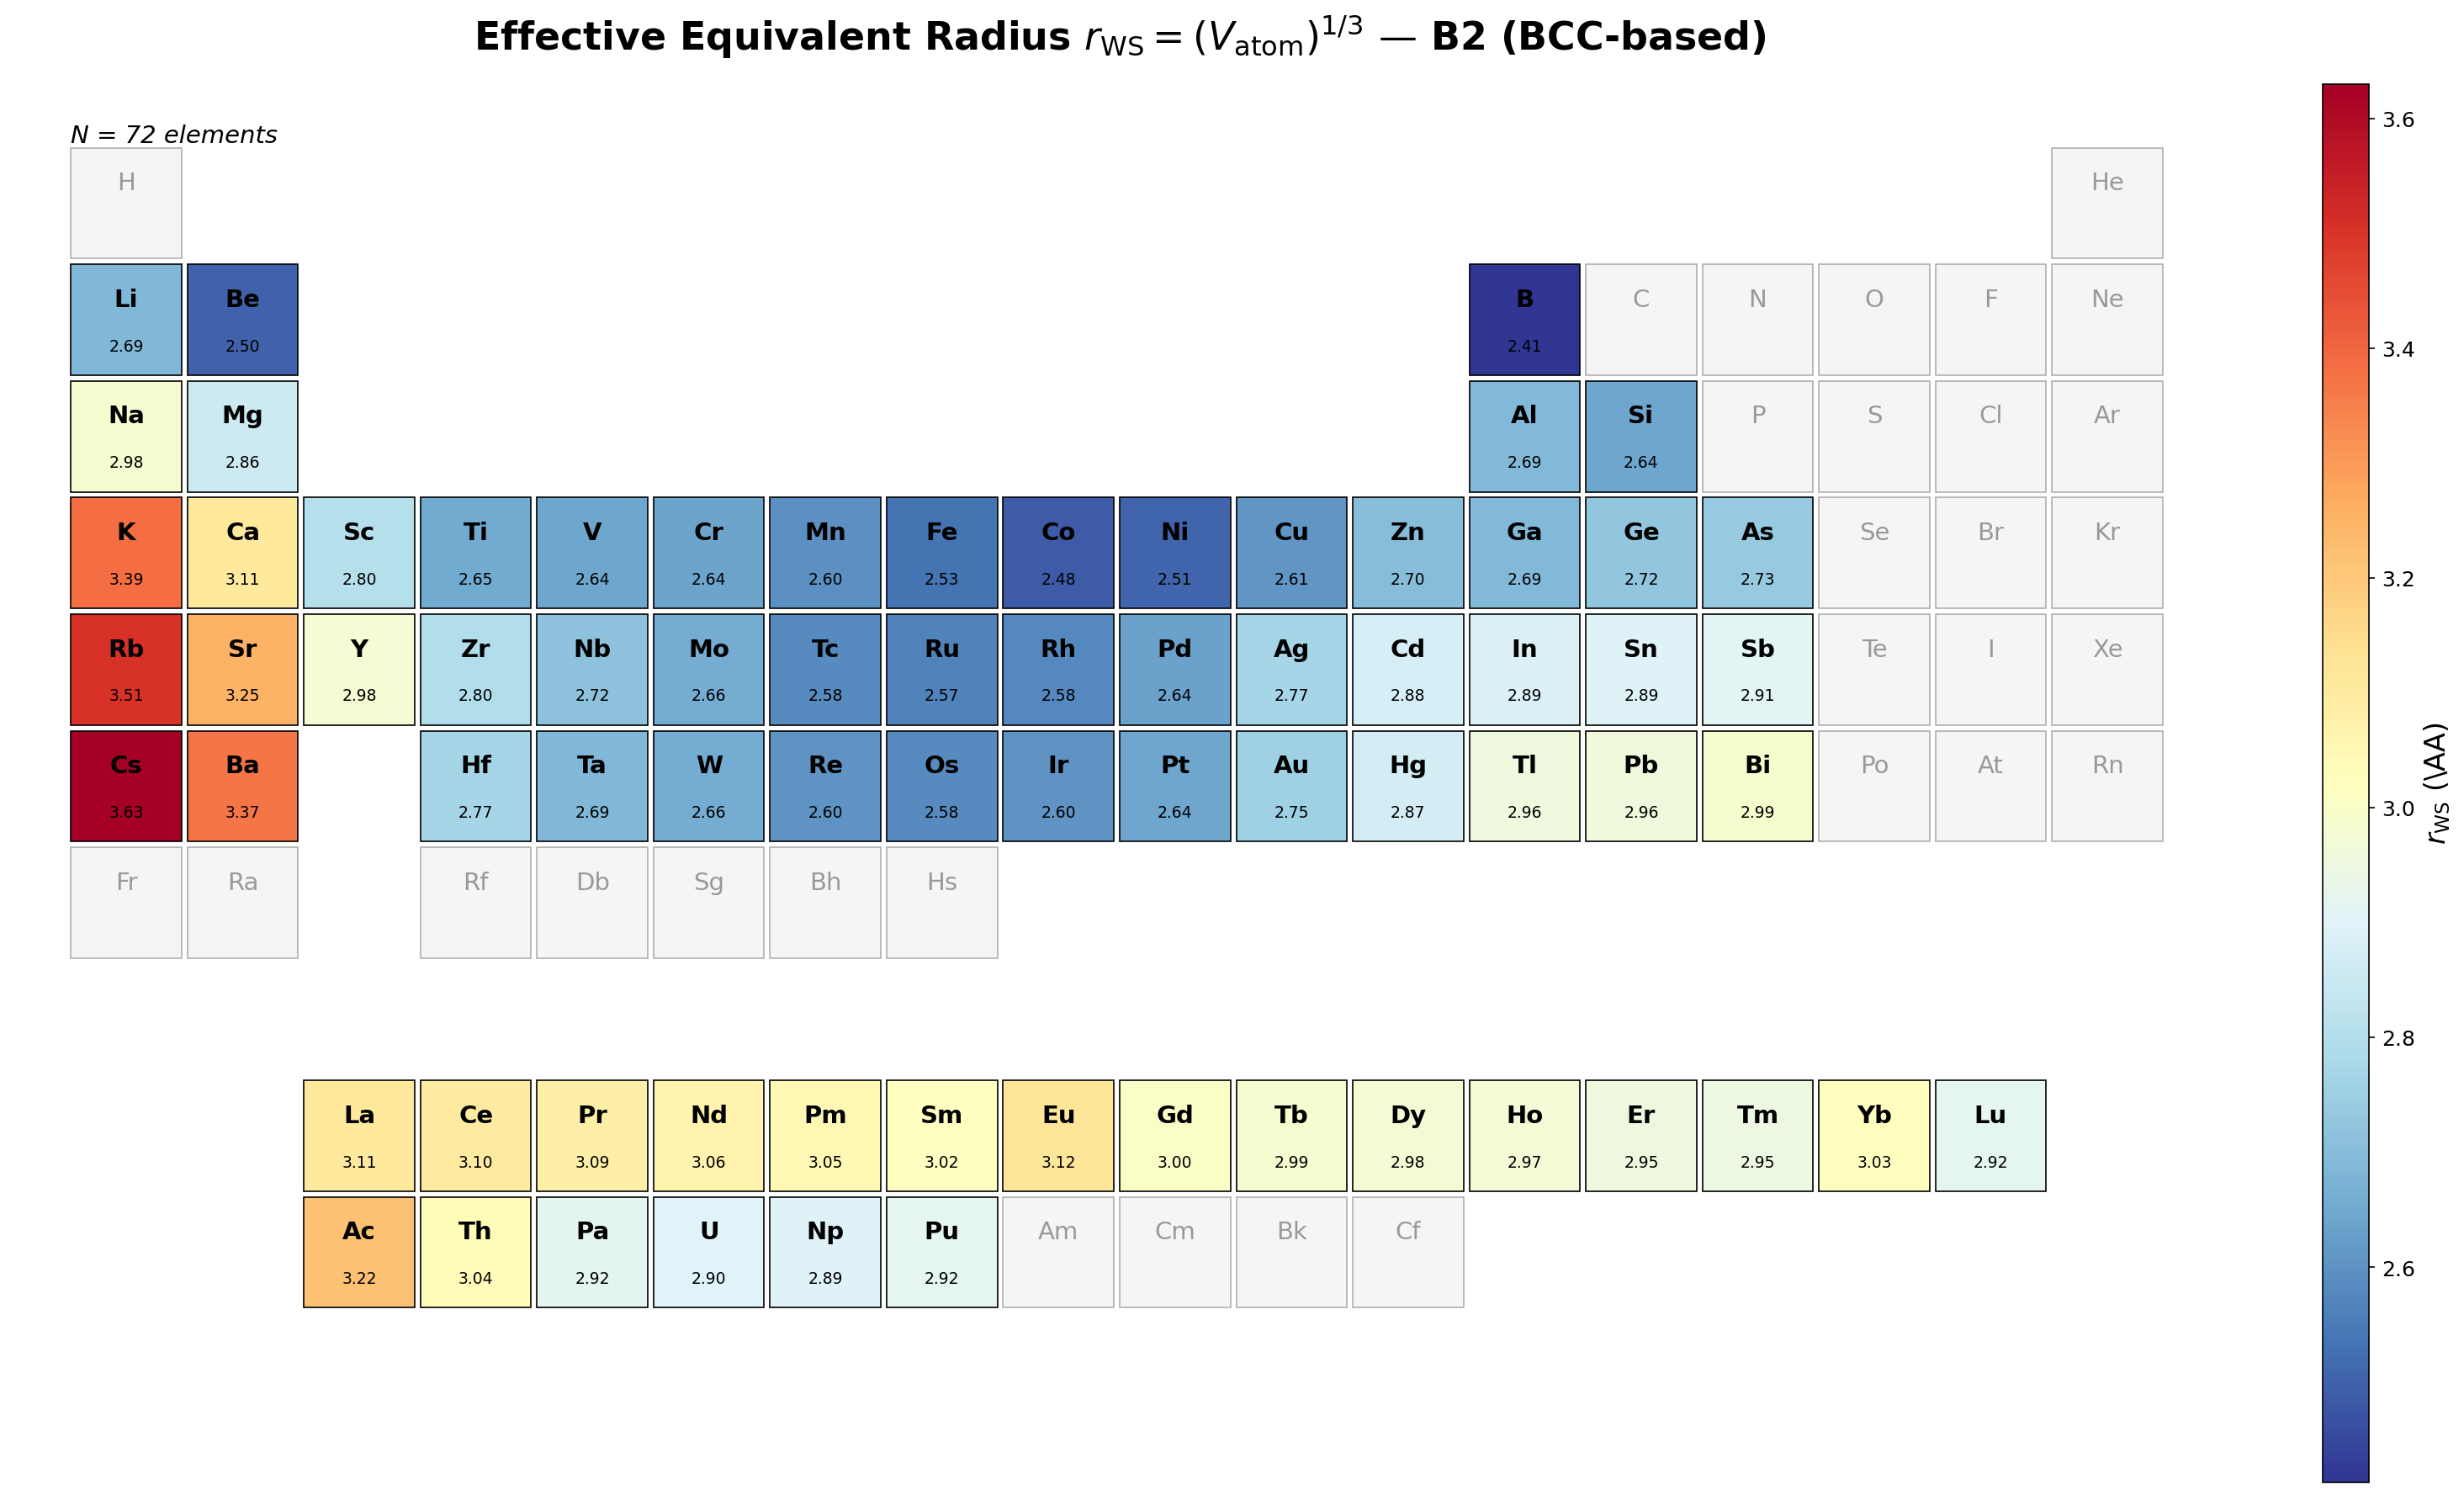
\includegraphics[width=0.95\linewidth]{periodic_table_rws_B2.png}
    \caption{B2化合物から算出した元素別$r_\mathrm{WS}$の周期表ヒートマップ。72元素。}
    \label{fig:periodic_rws_b2}
  \end{minipage}
  \hfill
  \begin{minipage}[t]{0.48\textwidth}
    \centering
    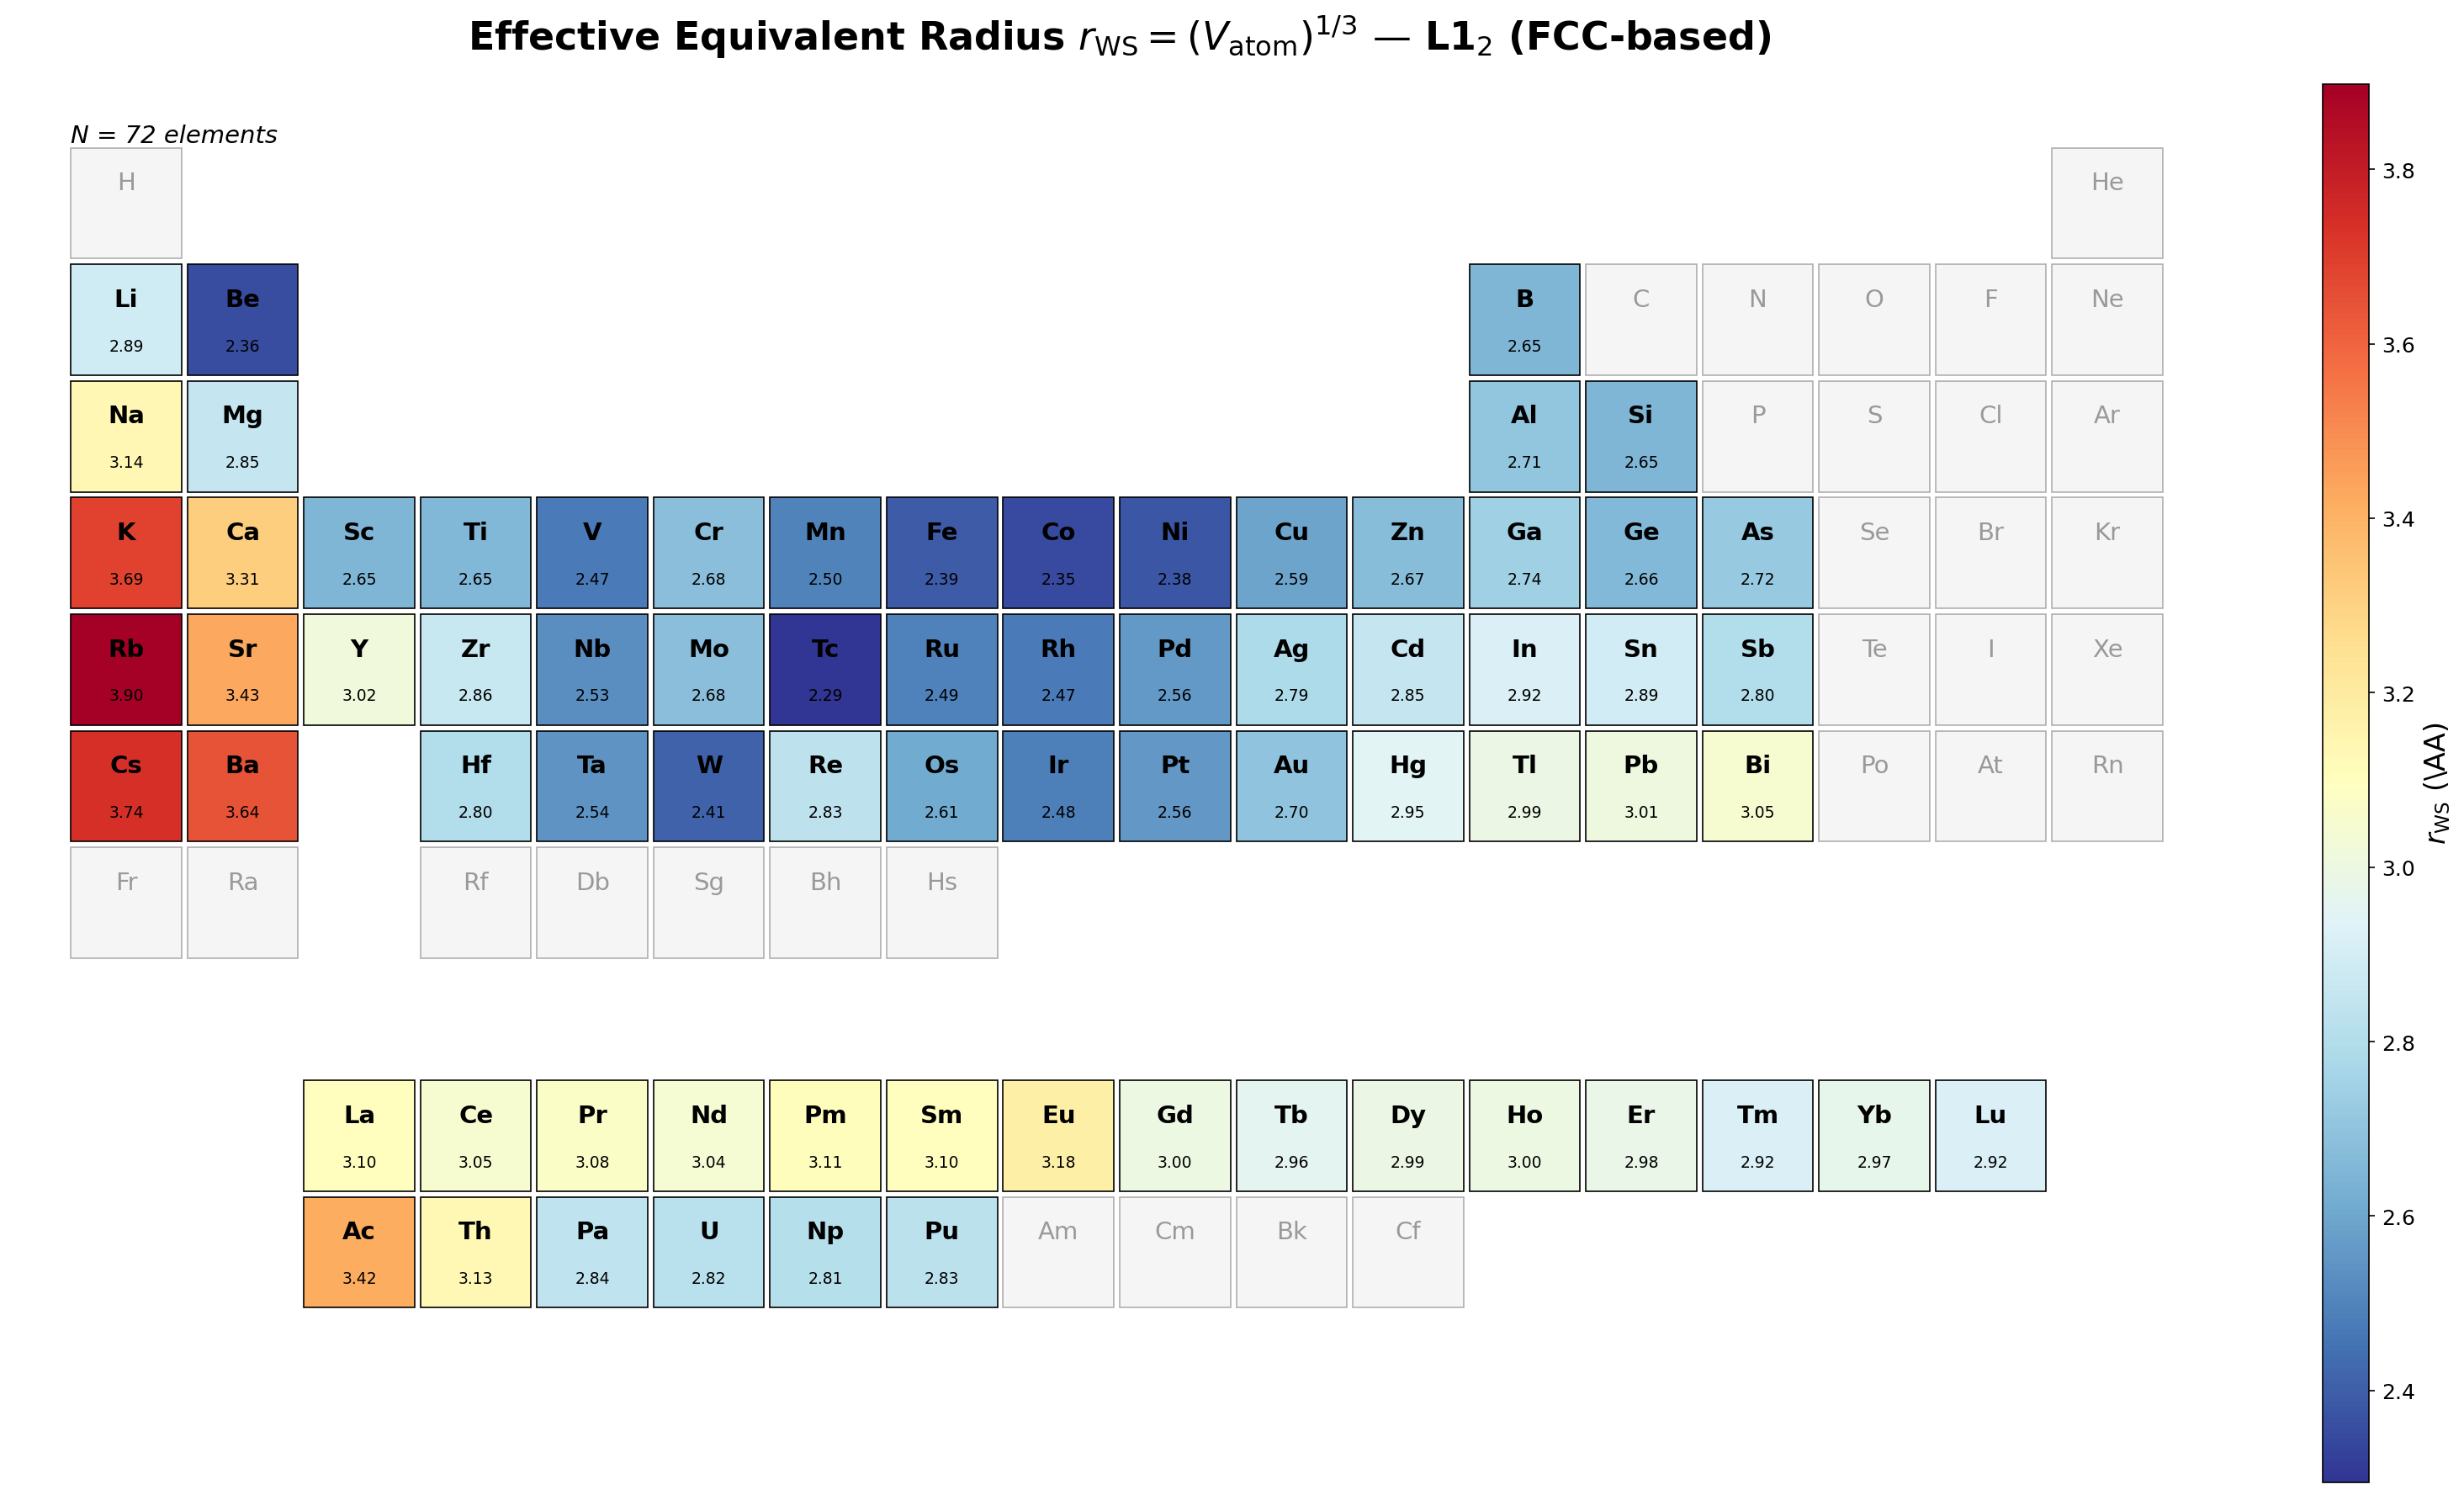
\includegraphics[width=0.95\linewidth]{periodic_table_rws_L12.png}
    \caption{L1$_2$化合物から算出した元素別$r_\mathrm{WS}$の周期表ヒートマップ。72元素。}
    \label{fig:periodic_rws_l12}
  \end{minipage}
\end{figure*}


\subsubsection{$r_\mathrm{contact}/r_\mathrm{WS}$比の周期表ヒートマップ}
接触半径とWigner--Seitz半径の比の元素分布を図~\ref{fig:periodic_ratio}に示す。比が1に近い元素は接触半径と$r_\mathrm{WS}$が一致することを意味する。ランタノイド（比$\approx 0.93$--$0.96$）は比較的高い一致度を示す一方、3d遷移金属（比$\approx 0.80$--$0.85$）では乖離が大きい。

\begin{figure*}[t]
  \centering
  \begin{minipage}[t]{0.48\textwidth}
    \centering
    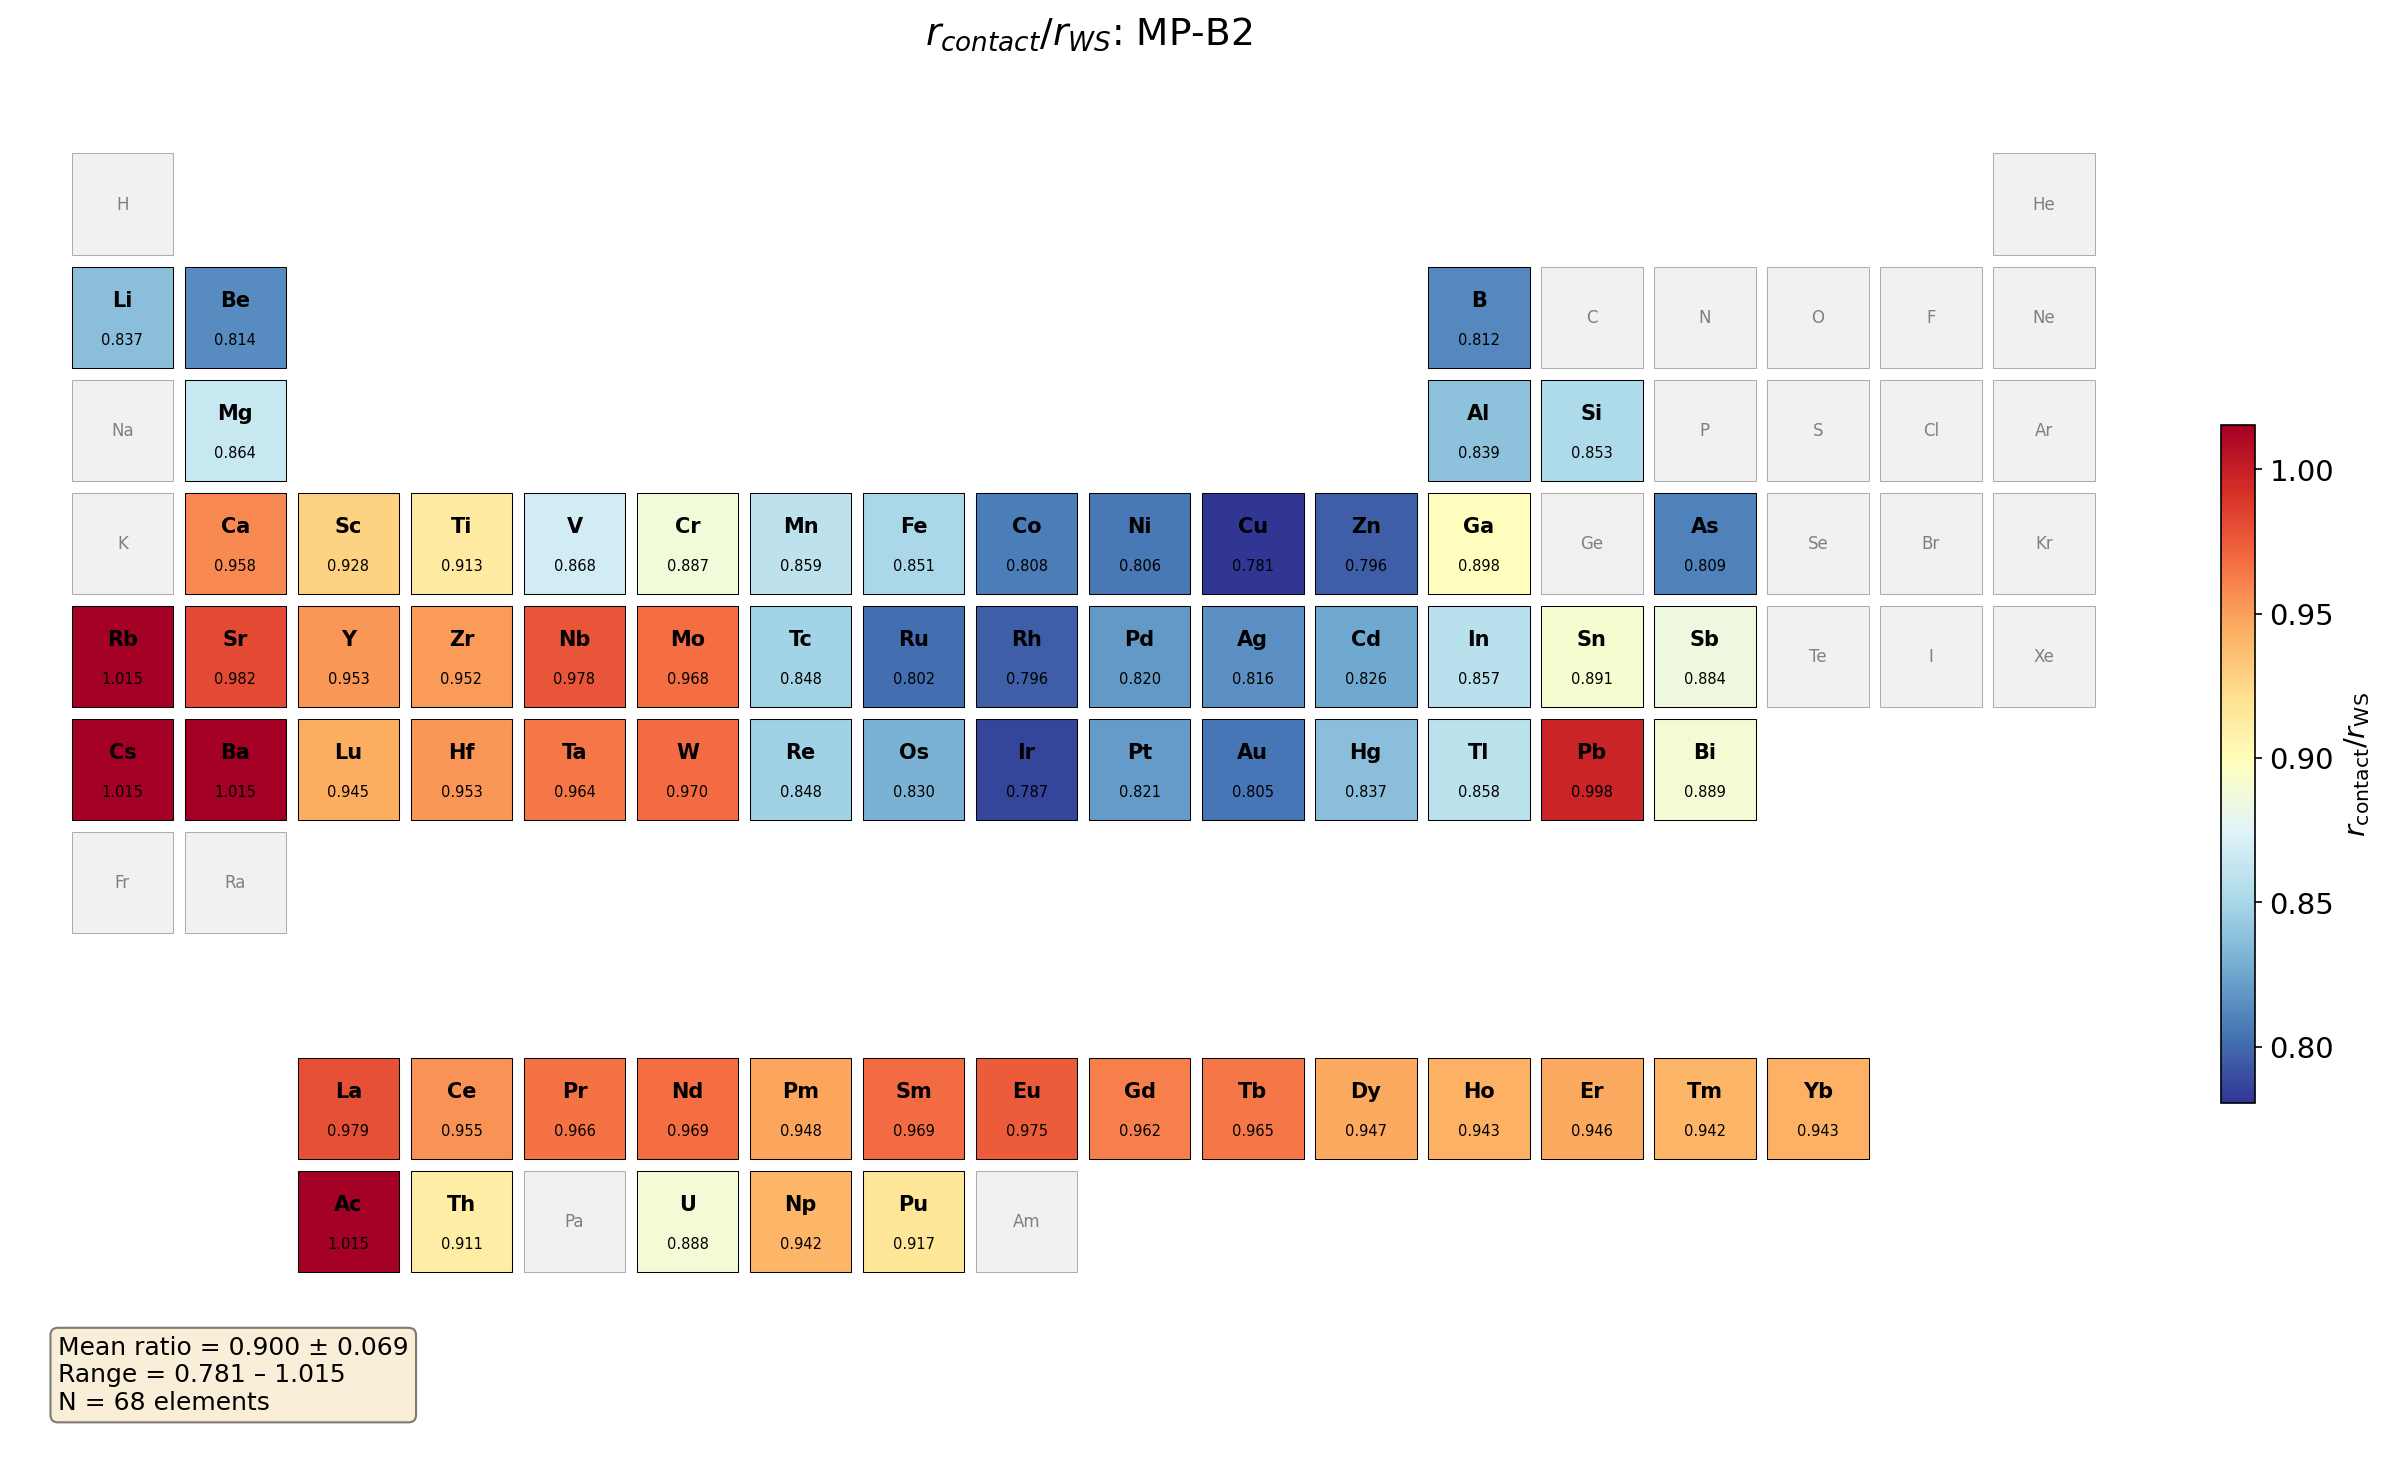
\includegraphics[width=0.95\linewidth]{periodic_ratio_MP_B2.png}
    \caption{MP-B2: $r_\mathrm{contact}/r_\mathrm{WS}$比の周期表ヒートマップ。平均比 = 0.900。}
    \label{fig:periodic_ratio_mp_b2}
  \end{minipage}
  \hfill
  \begin{minipage}[t]{0.48\textwidth}
    \centering
    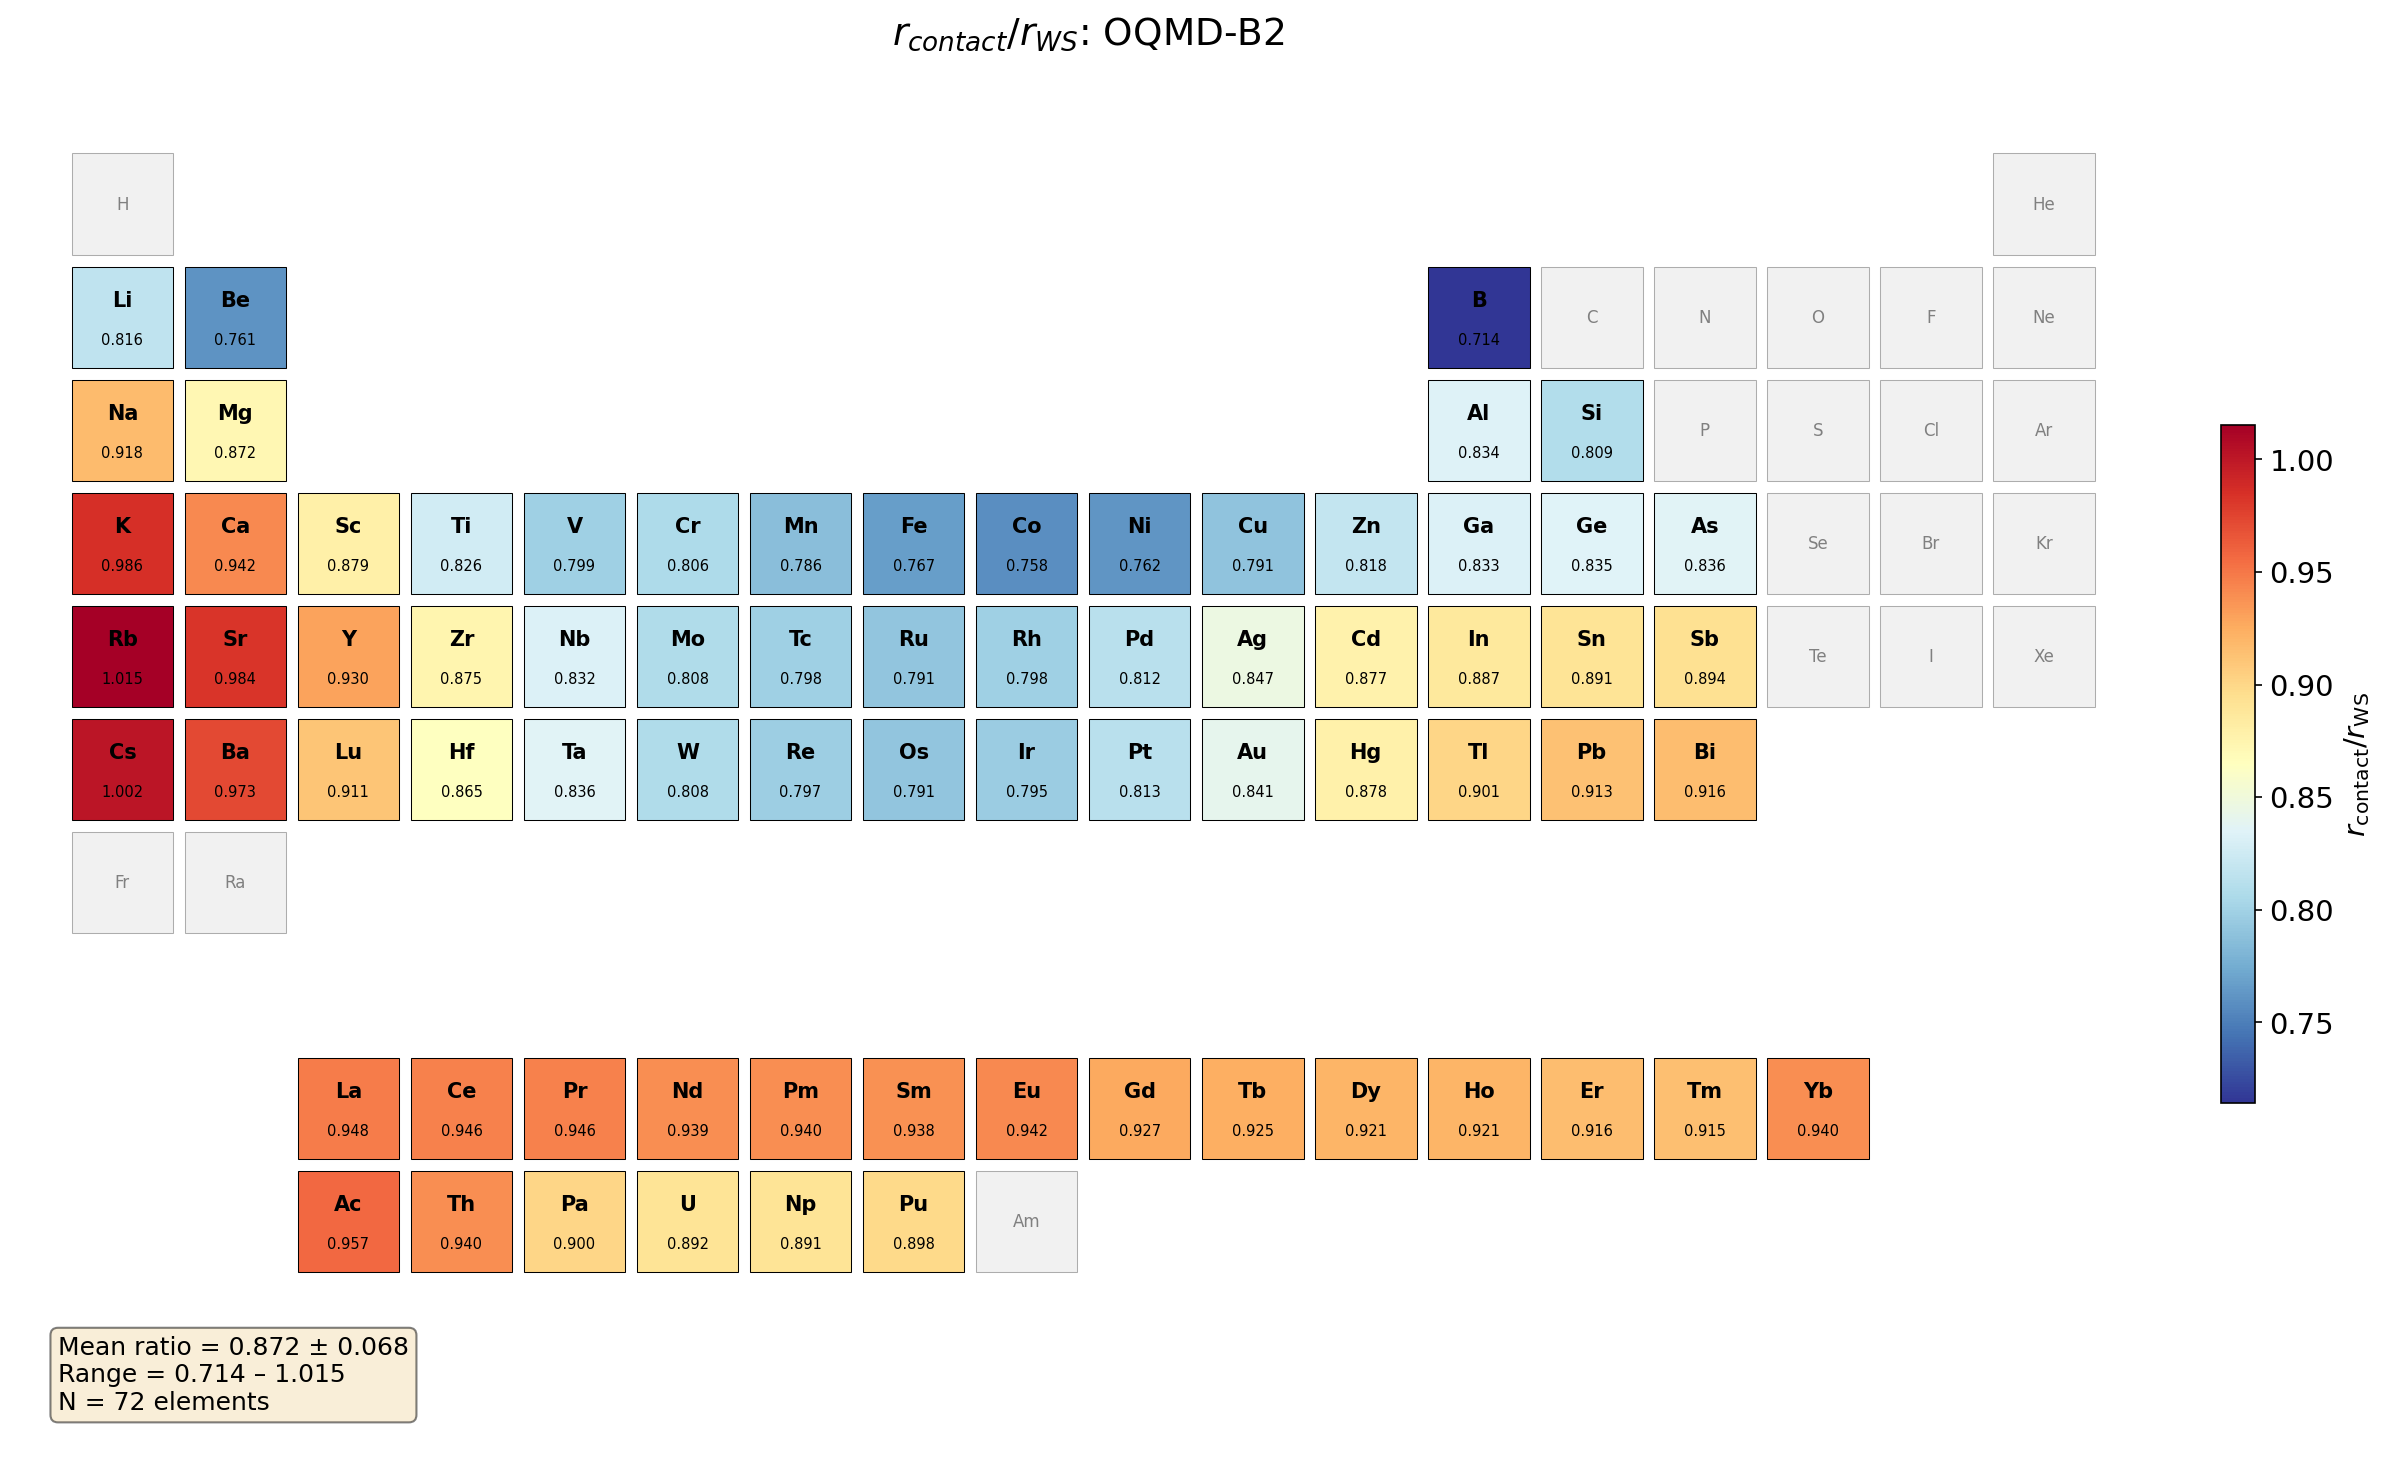
\includegraphics[width=0.95\linewidth]{periodic_ratio_OQMD_B2.png}
    \caption{OQMD-B2: $r_\mathrm{contact}/r_\mathrm{WS}$比の周期表ヒートマップ。平均比 = 0.872。}
    \label{fig:periodic_ratio_oqmd_b2}
  \end{minipage}
\end{figure*}


\subsubsection{$r_\mathrm{WS}$の構造依存性: B2 vs L1$_2$}
図~\ref{fig:rws_b2_vs_l12}に、同一元素について$r_\mathrm{WS}$(B2) vs $r_\mathrm{WS}$(L1$_2$)の散布図を示す。トレンドから大きく外れるアウトライヤーは赤太字でラベル表示されている。

MP（図~\ref{fig:rws_b2l12_mp}）では平均差$-3.81$\%（B2がL1$_2$より小さい）、OQMD（図~\ref{fig:rws_b2l12_oqmd}）では平均差$+6.39$\%（B2がL1$_2$より大きい）であり、データベース間で符号が逆転している。これは、$r_\mathrm{WS}$がDFT格子定数から直接算出されるため、MPとOQMDの計算パラメータ差（特にL1$_2$データの元素分布の差異）を反映していると考えられる。

\begin{figure*}[t]
  \centering
  \begin{minipage}[t]{0.48\textwidth}
    \centering
    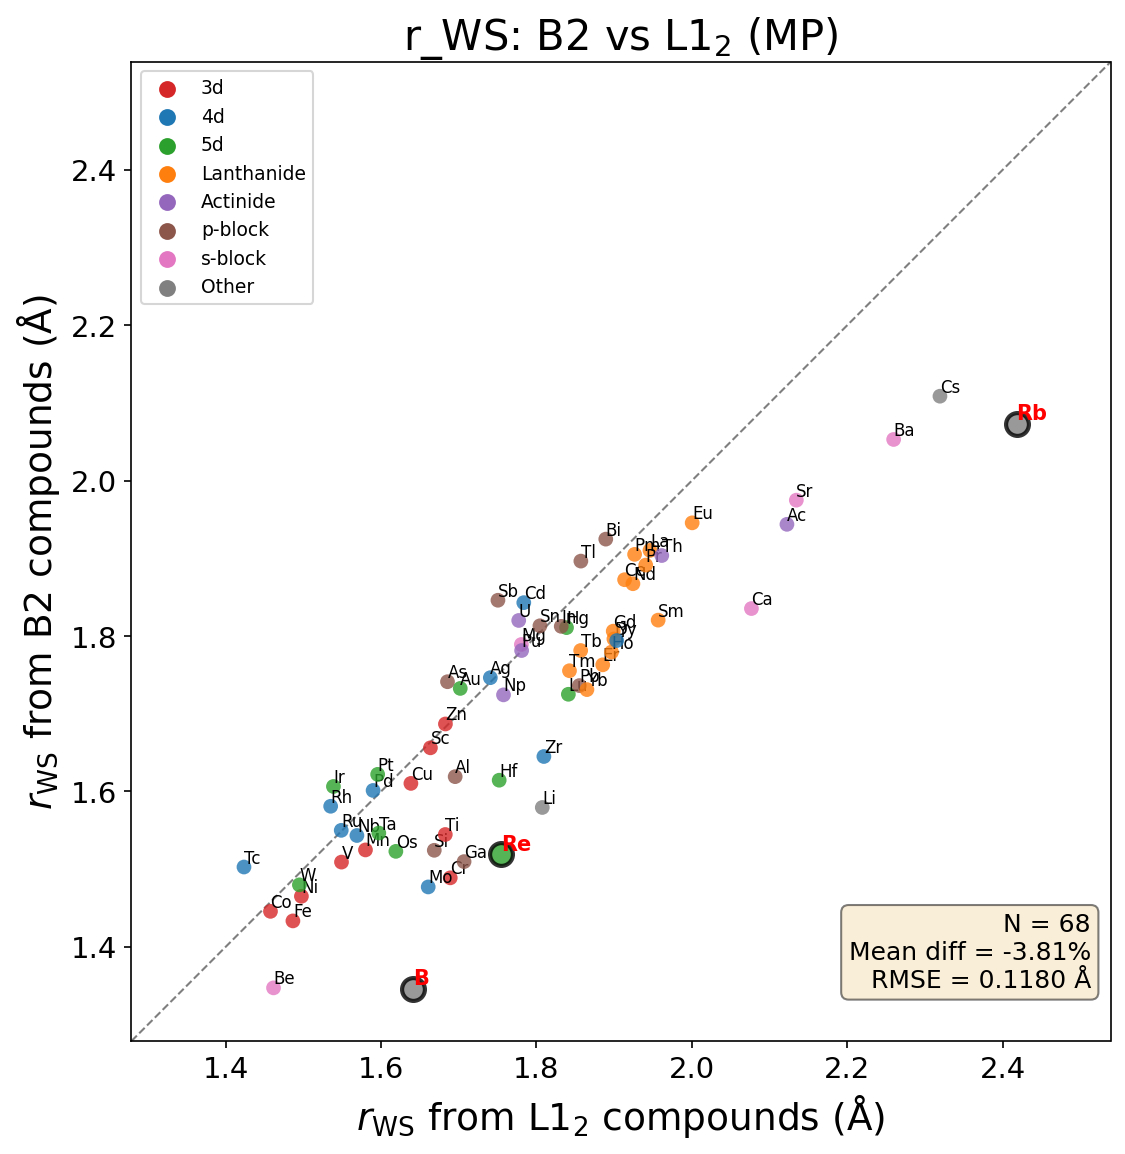
\includegraphics[width=0.95\linewidth]{rws_B2_vs_L12_MP.png}
    \caption{MP: $r_\mathrm{WS}$(B2) vs $r_\mathrm{WS}$(L1$_2$)。平均差 = $-$3.81\%。赤太字ラベルはアウトライヤー。}
    \label{fig:rws_b2l12_mp}
  \end{minipage}
  \hfill
  \begin{minipage}[t]{0.48\textwidth}
    \centering
    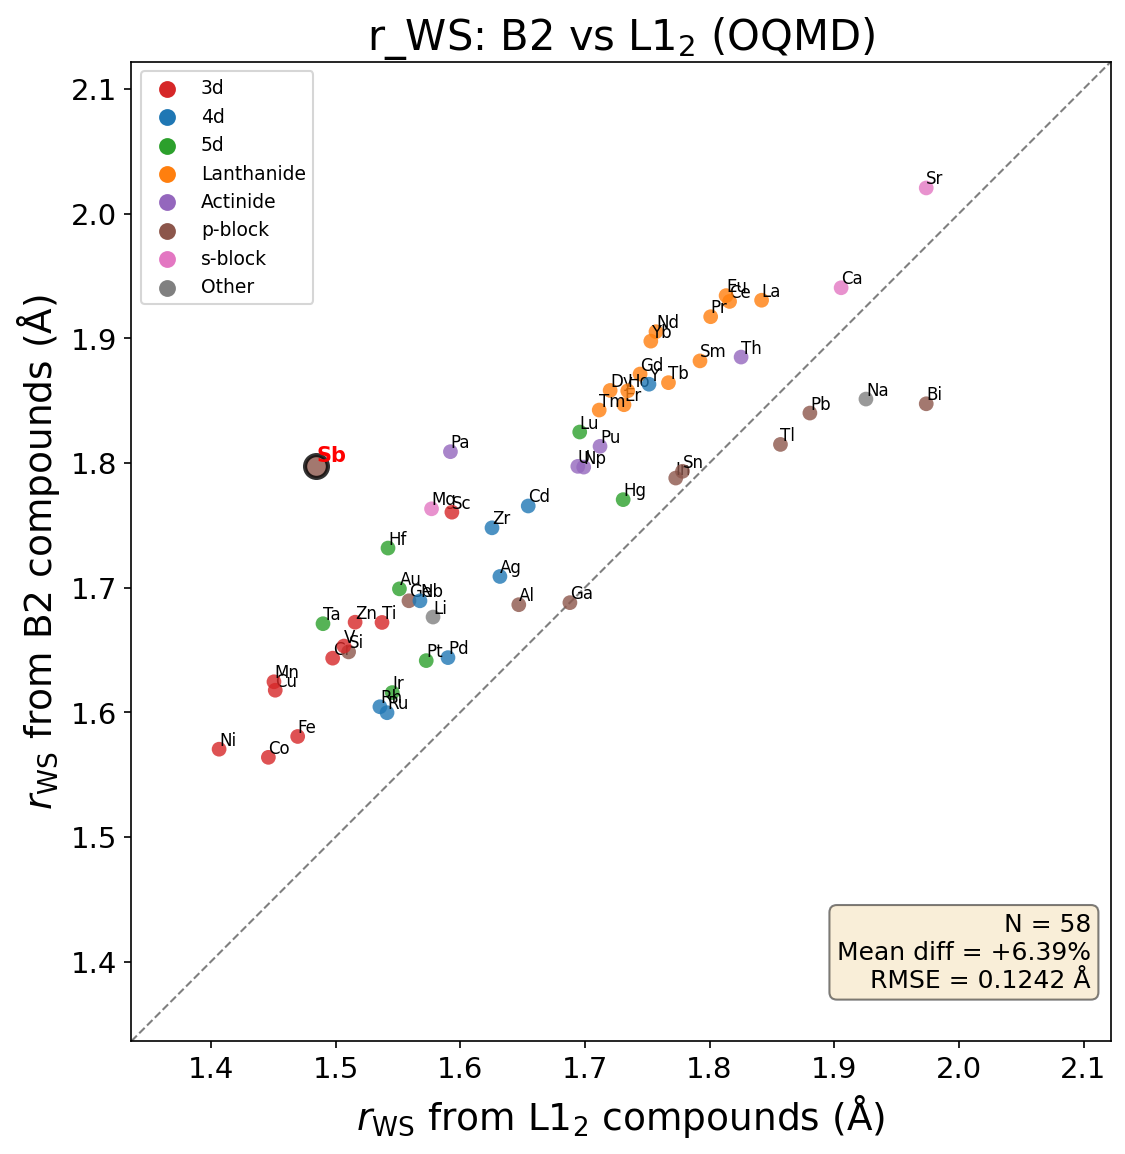
\includegraphics[width=0.95\linewidth]{rws_B2_vs_L12_OQMD.png}
    \caption{OQMD: $r_\mathrm{WS}$(B2) vs $r_\mathrm{WS}$(L1$_2$)。平均差 = $+$6.39\%。}
    \label{fig:rws_b2l12_oqmd}
  \end{minipage}
\end{figure*}


\subsubsection{元素群別$r_\mathrm{contact}/r_\mathrm{WS}$比の箱ひげ図}
図~\ref{fig:group_ratio}に元素群別の$r_\mathrm{contact}/r_\mathrm{WS}$比の箱ひげ図を示す。ランタノイドが最も高い比（$\approx 0.93$）を示し、3d遷移金属が最も低い比（$\approx 0.80$--$0.85$）を示す傾向は、全4ケースで共通している。

\begin{figure*}[t]
  \centering
  \begin{minipage}[t]{0.48\textwidth}
    \centering
    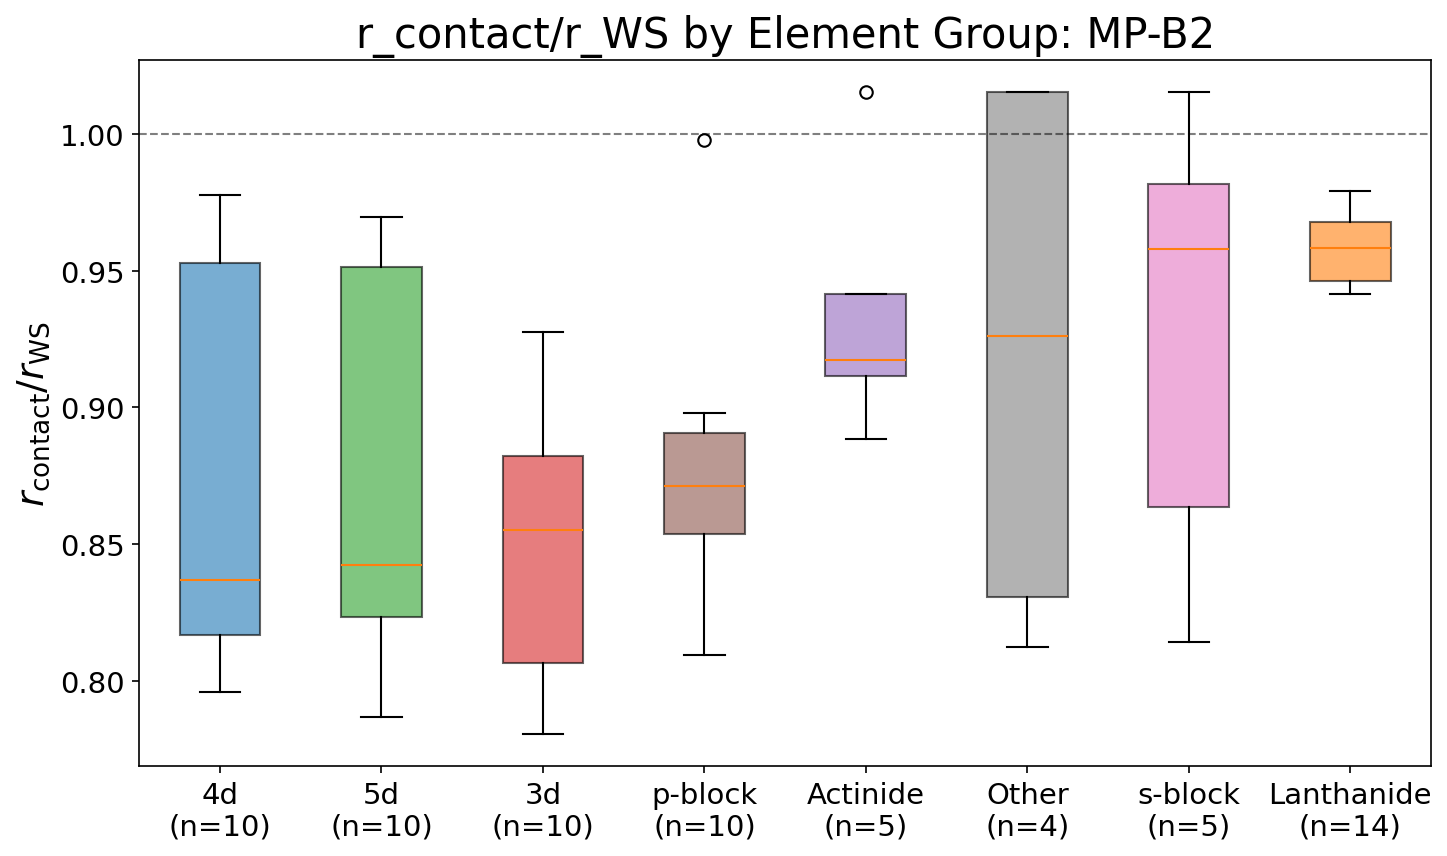
\includegraphics[width=0.95\linewidth]{group_ratio_MP_B2.png}
    \caption{MP-B2: 元素群別$r_\mathrm{contact}/r_\mathrm{WS}$比の箱ひげ図。}
    \label{fig:group_ratio_mp_b2}
  \end{minipage}
  \hfill
  \begin{minipage}[t]{0.48\textwidth}
    \centering
    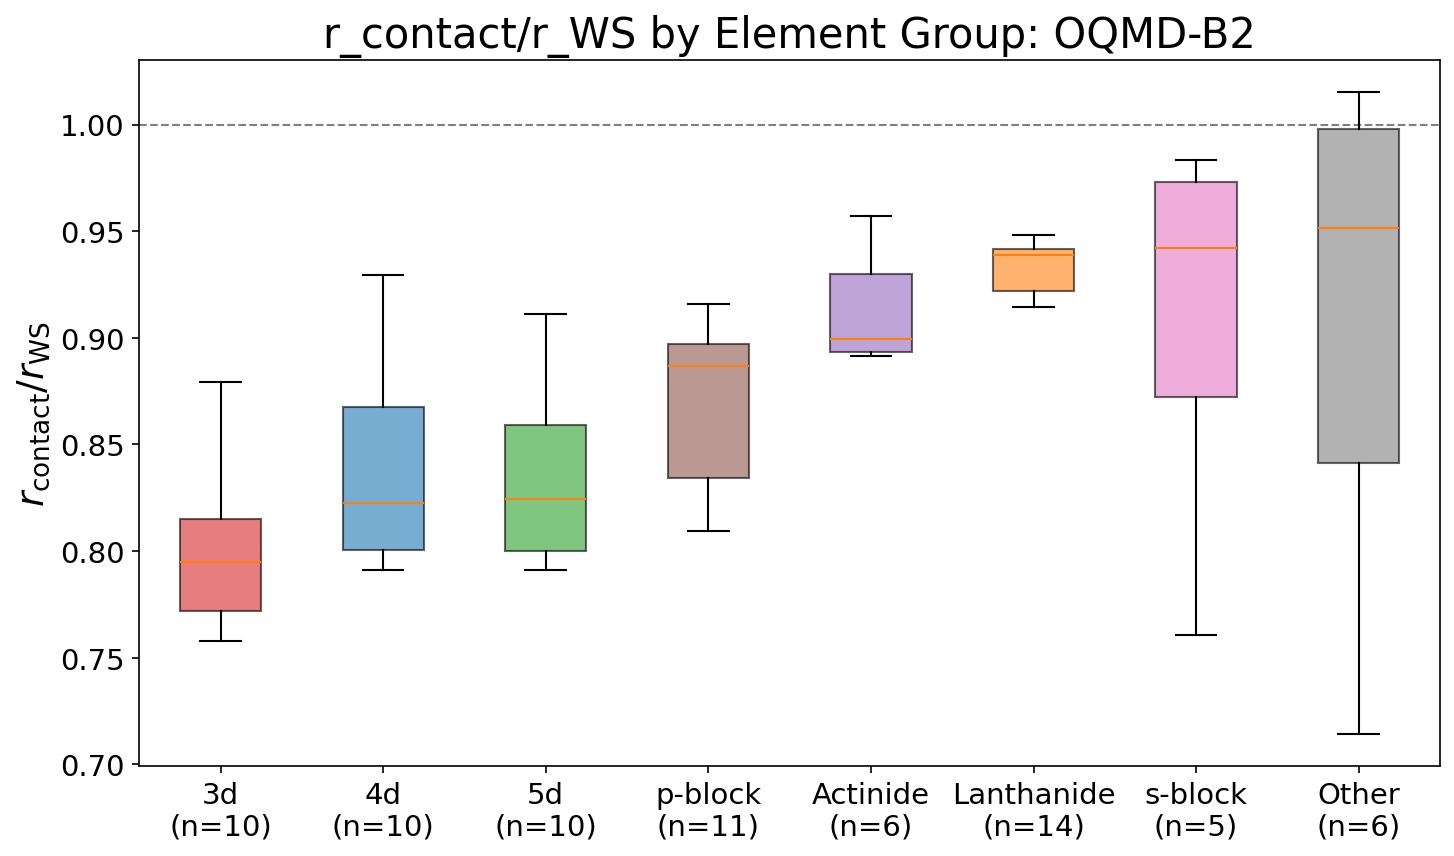
\includegraphics[width=0.95\linewidth]{group_ratio_OQMD_B2.png}
    \caption{OQMD-B2: 元素群別$r_\mathrm{contact}/r_\mathrm{WS}$比の箱ひげ図。}
    \label{fig:group_ratio_oqmd_b2}
  \end{minipage}
\end{figure*}


\subsection{実験格子定数との比較}
最適化された有効半径の妥当性を検証するため、代表的なB2化合物12件およびL1$_2$化合物9件について、実験格子定数（Pearson's Handbook~\cite{villars1991}）とMP/OQMDそれぞれのDFT計算値およびモデル予測値を比較した（表~\ref{tab:exp_comparison}）。

B2化合物に対するモデル予測誤差の平均は、MP半径で1.5\%、OQMD半径で2.0\%であった。FeCo が最大誤差（MP: $-3.5$\%、OQMD: $-3.9$\%）を示し、磁性元素同士の電子効果を反映している。Pauling半径による平均誤差は4.4\%であり、系統的な過大評価を示した。

L1$_2$化合物では、MnNi$_3$を除く7件で平均誤差1.1--1.3\%と良好な一致を示した。MnNi$_3$の大きな誤差（MP: $-8.7$\%）はMnの磁気的相互作用の影響と考えられる。

\begin{table*}[htbp]
\centering
\caption{代表的B2およびL1$_2$化合物の実験格子定数とDFT計算値・モデル予測値の比較。実験値はPearson's Handbook~\cite{villars1991}より。従来半径: B2にPauling半径~\cite{pauling1947}、L1$_2$にGoldschmidt半径~\cite{goldschmidt1927}。}
\label{tab:exp_comparison}
\scalebox{0.75}{
\begin{tabular}{llcccccccccccc}
\toprule
 & & & \multicolumn{2}{c}{DFT (\AA)} & \multicolumn{2}{c}{モデル (\AA)} & 従来 & \multicolumn{2}{c}{Err$_\mathrm{DFT}$ (\%)} & \multicolumn{2}{c}{Err$_\mathrm{model}$ (\%)} & Err$_\mathrm{conv}$ \\
\cmidrule(lr){4-5} \cmidrule(lr){6-7} \cmidrule(lr){9-10} \cmidrule(lr){11-12}
構造 & 化合物 & $a_\mathrm{exp}$ & MP & OQMD & MP & OQMD & (\AA) & MP & OQMD & MP & OQMD & (\%) \\
\midrule
\multirow{12}{*}{B2} & AlNi & 2.887 & 2.860 & 2.886 & 2.932 & 2.997 & 3.095 & $-$0.9 & $-$0.0 & +1.6 & +3.8 & +7.2 \\
 & AlFe & 2.909 & 2.846 & 2.869 & 2.977 & 3.000 & 3.106 & $-$2.2 & $-$1.4 & +2.3 & +3.1 & +6.8 \\
 & AlCo & 2.862 & 2.819 & 2.846 & 2.917 & 2.978 & 3.095 & $-$1.5 & $-$0.6 & +1.9 & +4.0 & +8.1 \\
 & TiNi & 3.015 & 2.988 & 3.003 & 2.992 & 2.981 & 3.141 & $-$0.9 & $-$0.4 & $-$0.8 & $-$1.1 & +4.2 \\
 & TiFe & 2.976 & 2.939 & 2.939 & 3.037 & 2.983 & 3.152 & $-$1.3 & $-$1.2 & +2.1 & +0.2 & +5.9 \\
 & TiPd & 3.180 & 3.176 & 3.162 & 3.145 & 3.146 & 3.279 & $-$0.1 & $-$0.6 & $-$1.1 & $-$1.1 & +3.1 \\
 & TiPt & 3.192 & 3.179 & 3.167 & 3.166 & 3.145 & 3.302 & $-$0.4 & $-$0.8 & $-$0.8 & $-$1.5 & +3.5 \\
 & TiAu & 3.259 & 3.279 & 3.257 & 3.240 & 3.255 & 3.360 & +0.6 & $-$0.1 & $-$0.6 & $-$0.1 & +3.1 \\
 & FeCo & 2.857 & 2.839 & 2.779 & 2.757 & 2.747 & 2.898 & $-$0.6 & $-$2.7 & $-$3.5 & $-$3.9 & +1.4 \\
 & CuPd & 2.988 & 2.980 & 3.009 & 2.967 & 3.018 & 3.060 & $-$0.3 & +0.7 & $-$0.7 & +1.0 & +2.4 \\
 & HfCo & 3.164 & 3.163 & 3.138 & 3.126 & 3.098 & 3.279 & $-$0.0 & $-$0.8 & $-$1.2 & $-$2.1 & +3.6 \\
 & ZrCo & 3.196 & 3.208 & 3.163 & 3.157 & 3.131 & 3.291 & +0.4 & $-$1.0 & $-$1.2 & $-$2.0 & +3.0 \\
\midrule
\multirow{9}{*}{L1$_2$} & AlNi$_3$ & 3.572 & 3.523 & 3.556 & 3.492 & 3.638 & 3.790 & $-$1.4 & $-$0.4 & $-$2.2 & +1.8 & +6.1 \\
 & Cu$_3$Au & 3.748 & 3.735 & 3.767 & 3.690 & 3.812 & 3.847 & $-$0.3 & +0.5 & $-$1.5 & +1.7 & +2.6 \\
 & TiAl$_3$ & 3.967 & 3.956 & 3.979 & 3.968 & 3.973 & 4.101 & $-$0.3 & +0.3 & +0.0 & +0.2 & +3.4 \\
 & TiCo$_3$ & 3.617 & 3.587 & 3.587 & 3.674 & 3.566 & 3.847 & $-$0.8 & $-$0.8 & +1.6 & $-$1.4 & +6.3 \\
 & TiPt$_3$ & 3.907 & 3.925 & 3.930 & 3.860 & 3.877 & 4.045 & +0.4 & +0.6 & $-$1.2 & $-$0.8 & +3.5 \\
 & GaNi$_3$ & 3.576 & 3.537 & 3.581 & 3.553 & 3.661 & 3.762 & $-$1.1 & +0.1 & $-$0.6 & +2.4 & +5.2 \\
 & MnNi$_3$ & 3.589 & 3.543 & 3.555 & 3.278 & 3.451 & 3.620 & $-$1.3 & $-$0.9 & $-$8.7 & $-$3.8 & +0.9 \\
 & Cu$_3$Pd & 3.676 & 3.666 & 3.708 & 3.466 & 3.616 & 3.748 & $-$0.3 & +0.9 & $-$5.7 & $-$1.6 & +1.9 \\
 & NbIr$_3$ & 3.880 & 3.913 & 3.918 & 3.901 & 3.899 & 4.002 & +0.9 & +1.0 & +0.5 & +0.5 & +3.2 \\
\bottomrule
\end{tabular}
}
\end{table*}


\subsection{HEA格子定数予測}
14種のHEA（FCC 8種、BCC 6種）に対するパリティプロットを図~\ref{fig:hea_parity}に、半径セット別のRMSE比較を図~\ref{fig:hea_rmse}に示す。

FCC HEAではペアワイズmax接触モデル（式~\ref{eq:fcc_pairwise}）の採用により、全有効半径セットがPauling半径を凌駕した。特にOQMD-B2半径でRMSE = 0.023~\AA を達成し、Pauling半径（0.073~\AA）の約1/3の誤差となった。AuCuNiPdPt（貴金属系）の追加により格子定数範囲が3.572--3.806~\AA に拡大し、検証の信頼性が向上した。

BCC HEAではOQMD-B2半径が最良（RMSE = 0.051~\AA）であり、これもPauling半径（0.089~\AA）を上回った。

\begin{figure*}[htbp]
    \centering
    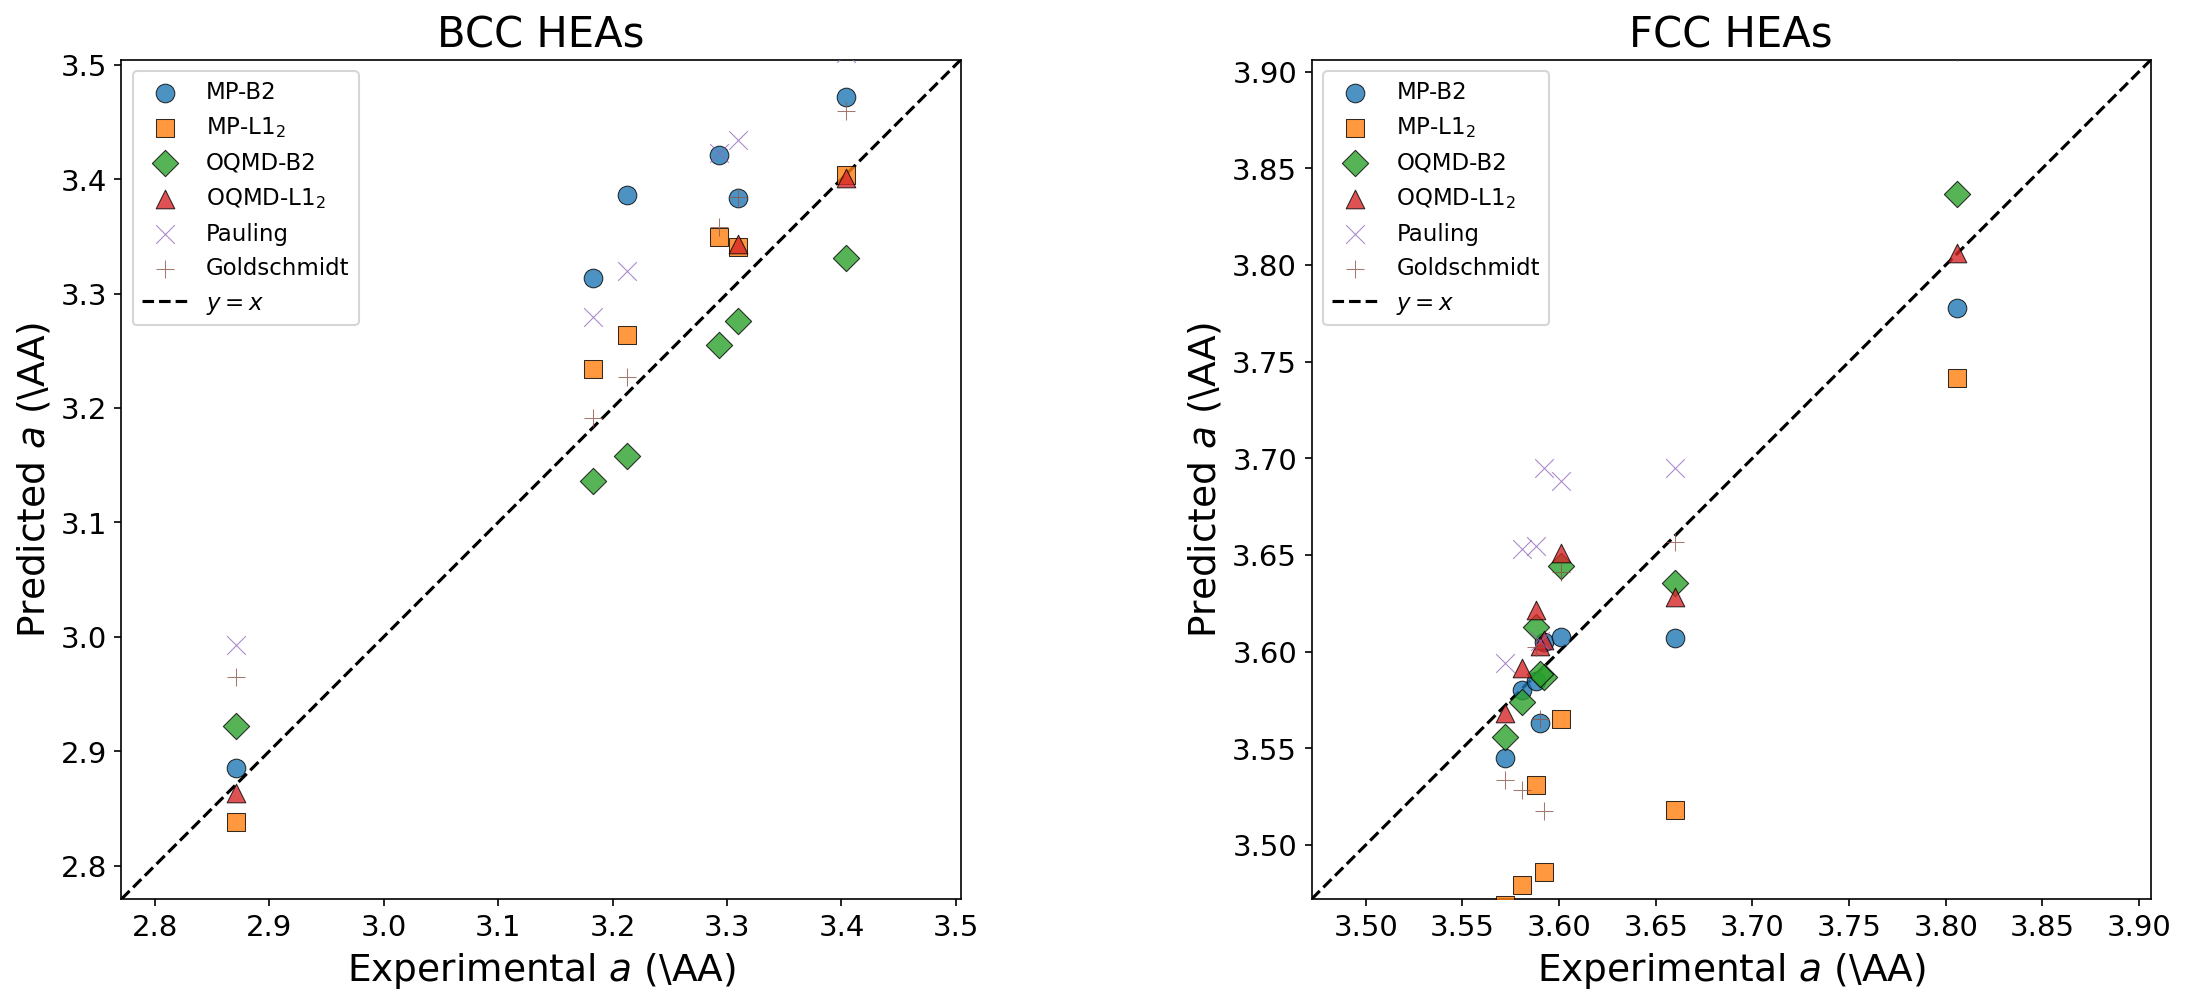
\includegraphics[width=0.95\textwidth]{hea_parity.png}
    \caption{HEA格子定数パリティプロット。左: BCC HEA（6種）、右: FCC HEA（8種）。各半径セット（MP-B2, MP-L1$_2$, OQMD-B2, OQMD-L1$_2$, Pauling, Goldschmidt）による予測値と実験値を比較。FCC HEAにはペアワイズmax接触モデルを使用。}
    \label{fig:hea_parity}
\end{figure*}

\begin{figure}[htbp]
    \centering
    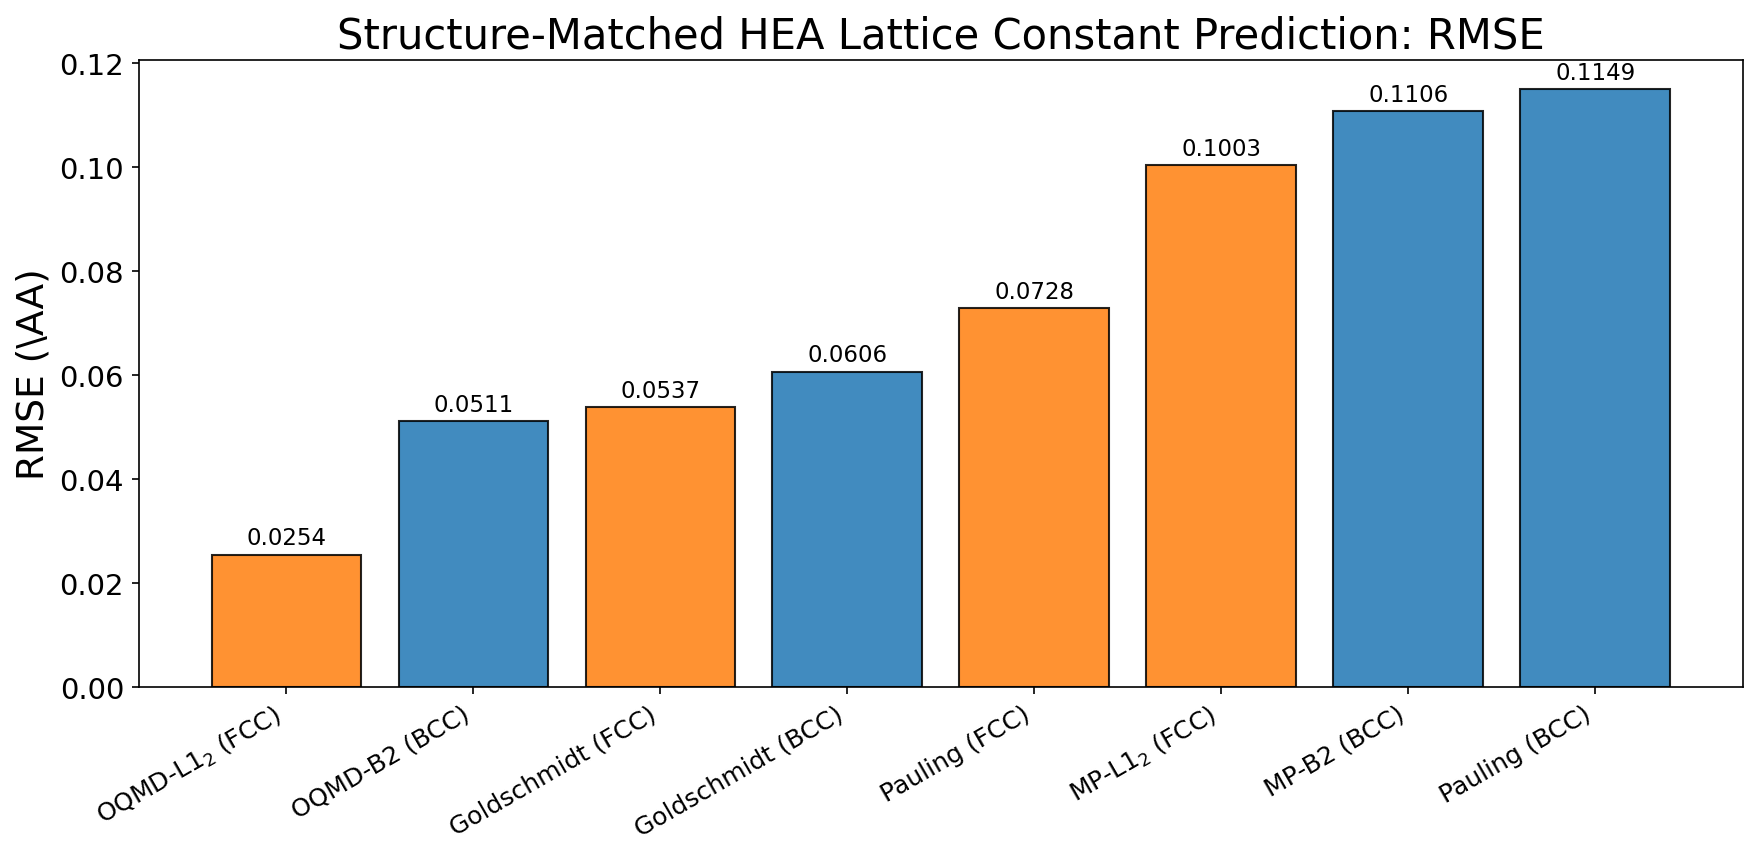
\includegraphics[width=0.45\textwidth]{hea_rmse_comparison.png}
    \caption{半径セット別のHEA格子定数予測RMSE。有効半径（特にOQMD-B2）がPauling半径を凌駕。}
    \label{fig:hea_rmse}
\end{figure}


\subsection{HEAの相図とサイズミスマッチ}
図~\ref{fig:hea_delta_vec}にHEAの$\delta$--VEC相図を示す。BCC HEA（$\delta < 6$\%、VEC $< 7$）とFCC HEA（$\delta < 6$\%、VEC $> 7$）が明確に分離される。有効半径から計算した$\delta$値が構造安定性の指標として有効に機能することを示す。

\begin{figure}[htbp]
    \centering
    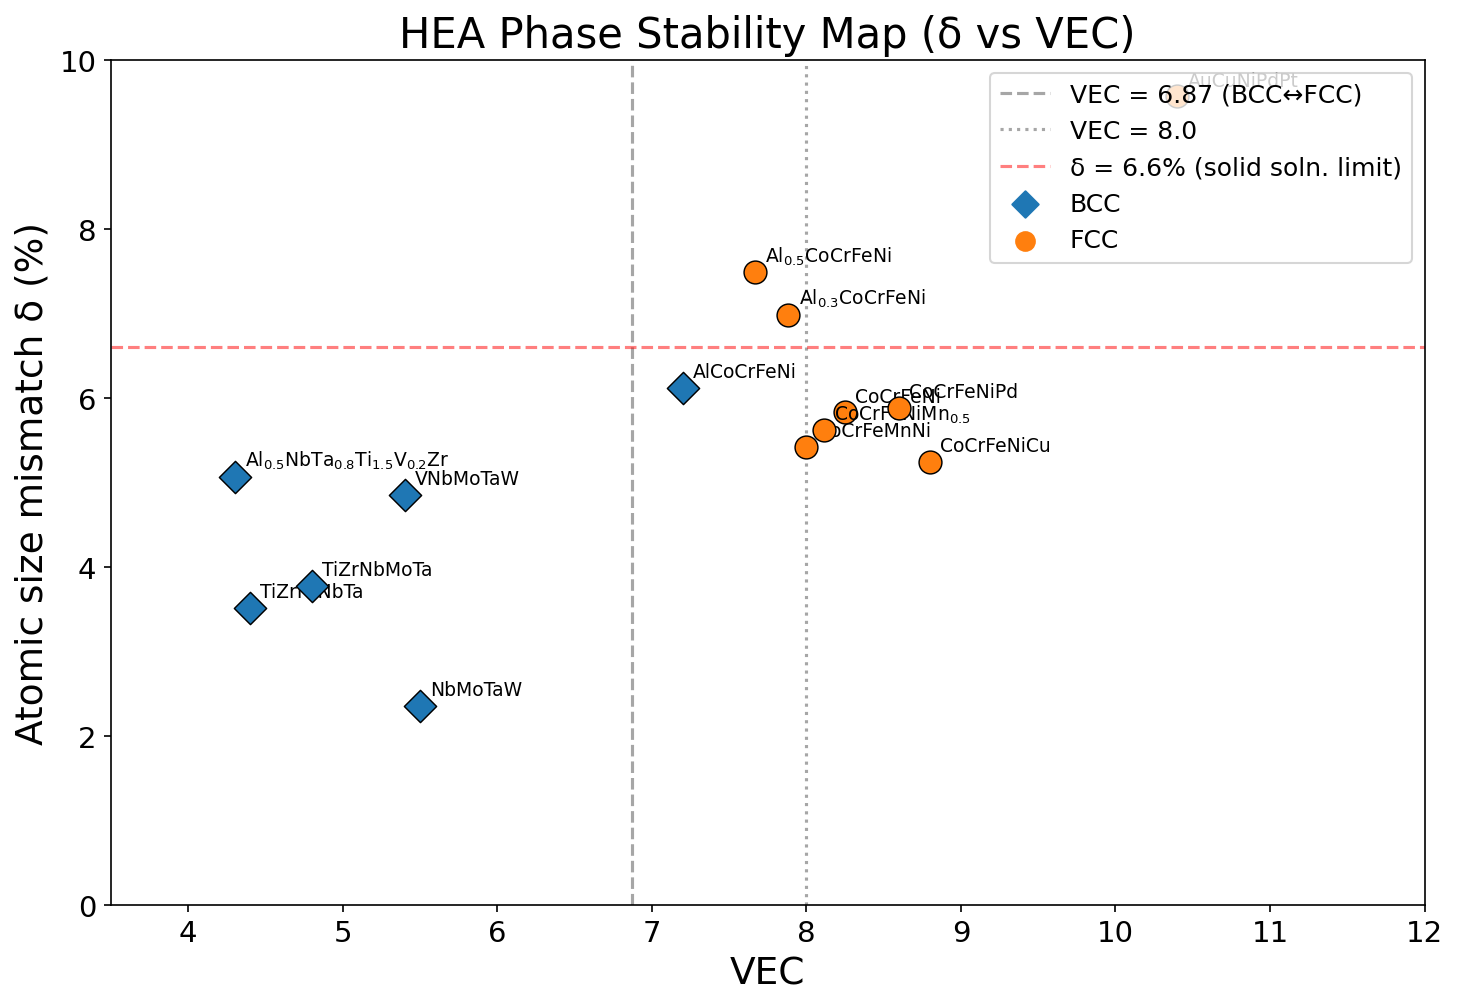
\includegraphics[width=0.45\textwidth]{hea_delta_vec_map.png}
    \caption{HEAの$\delta$--VEC相図。原子サイズミスマッチ$\delta$とVEC（価電子濃度）によるBCC/FCC構造の分類。}
    \label{fig:hea_delta_vec}
\end{figure}


\subsection{BMGガラス形成能評価}
図~\ref{fig:bmg_map}にBMG合金と結晶性HEAの$\delta$--$\lambda$マップを示す。BMG合金は$\delta > 6$\%の領域に、結晶性HEAは$\delta < 6$\%の領域にほぼ分離される。図~\ref{fig:bmg_delta_gfa}に$\delta$とガラス形成能の相関を示す。有効半径から算出した$\delta$がガラス形成合金を良好に識別できることを確認した。

\begin{figure*}[t]
  \centering
  \begin{minipage}[t]{0.48\textwidth}
    \centering
    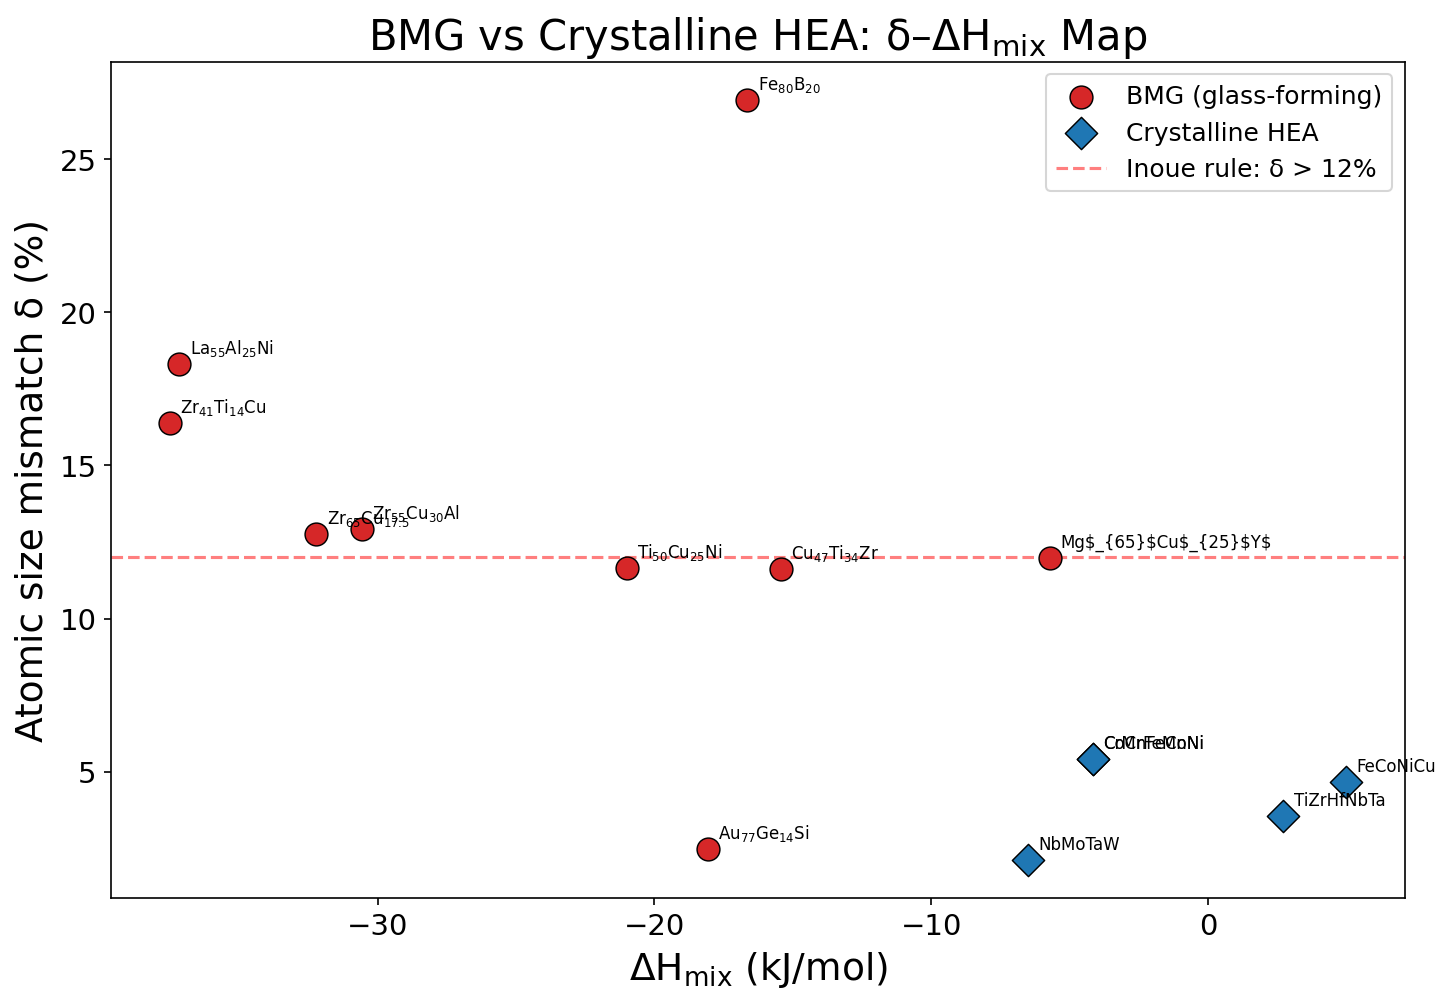
\includegraphics[width=0.95\linewidth]{bmg_vs_crystalline_map.png}
    \caption{BMG合金と結晶性HEAの$\delta$--$\lambda$マップ。$\delta > 6$\%（赤領域）にBMGが集中。}
    \label{fig:bmg_map}
  \end{minipage}
  \hfill
  \begin{minipage}[t]{0.48\textwidth}
    \centering
    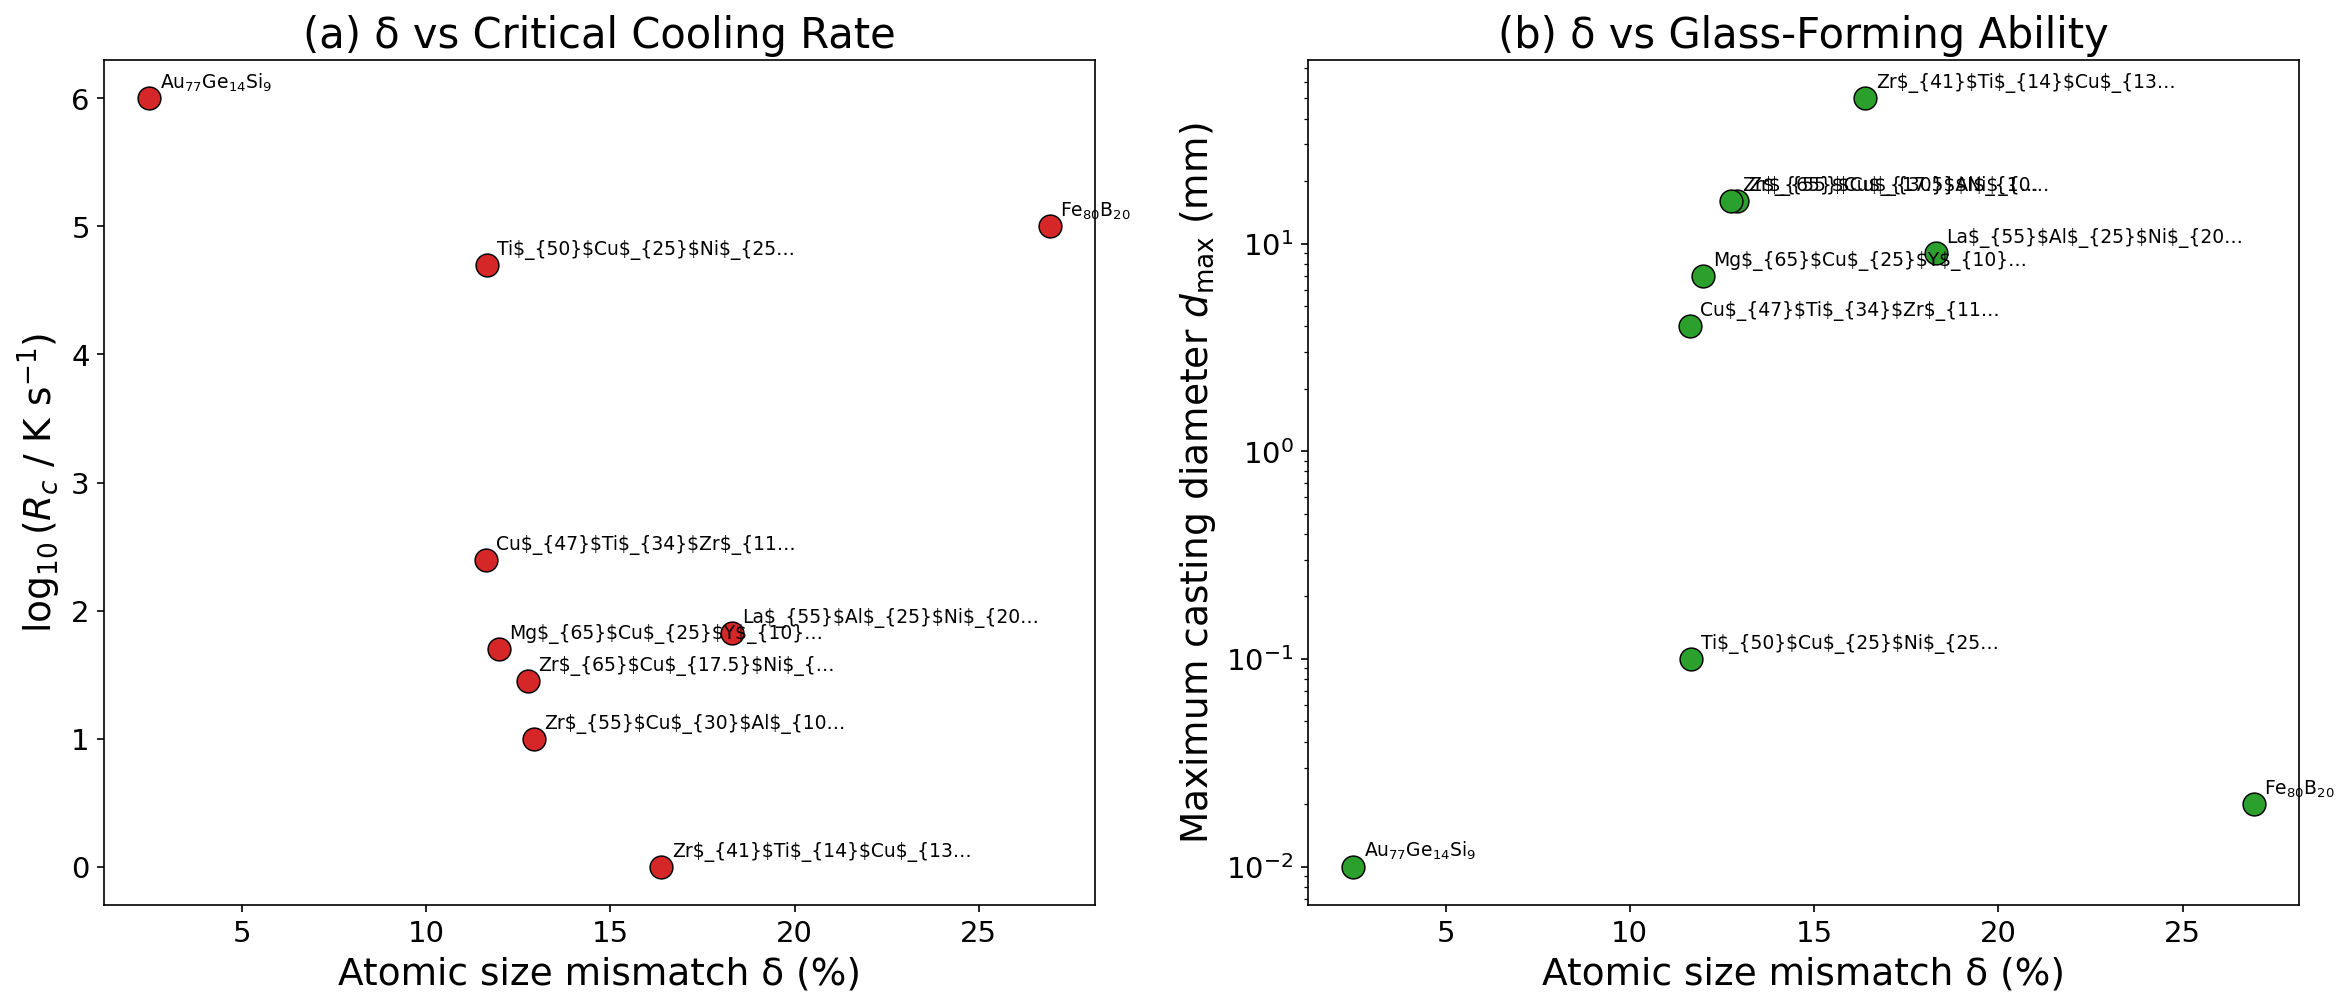
\includegraphics[width=0.95\linewidth]{bmg_delta_gfa.png}
    \caption{$\delta$とガラス形成能（GFA）の相関。有効半径から算出した$\delta$がBMG/結晶性合金を良好に分離する。}
    \label{fig:bmg_delta_gfa}
  \end{minipage}
\end{figure*}


%%%%%%%%%%%%%%%%%%%%%%%%%%%%%%%%%%%%%
\section{考察}

\subsection{非金属元素・アルカリ金属元素除外の効果}
非金属元素およびアルカリ金属元素を含む化合物の除外は剛体球モデルの精度に大きく影響する。非金属元素はイオン性・共有結合性が強く、剛体球近似が不適切である。アルカリ金属は大きなイオン半径と強いイオン性のため、B2構造において格子定数の系統的な過大評価を引き起こす。

\begin{table}[htbp]
\small
    \centering
    \caption{非金属・アルカリ金属除外の効果。Before RMSEは従来のA-B接触のみモデル（除外前）、After RMSEは本研究のmax基準モデル（除外後）。}
    \label{tab:nonmetal_effect}
\scalebox{0.9}{
    \begin{tabular}{lccc}
        \toprule
        ケース & Before RMSE (\AA) & After RMSE (\AA) & 改善率 \\
        \midrule
        MP-B2 & 0.158 & 0.054 & 66\% \\
        MP-L1$_2$ & 0.206 & 0.116 & 44\% \\
        OQMD-B2 & 0.102 & 0.095 & 7\% \\
        OQMD-L1$_2$ & 0.067 & 0.066 & 1\% \\
        \bottomrule
    \end{tabular}
    }
\end{table}


\subsection{有効接触半径の構造依存性}
表~\ref{tab:element_groups}のB2--L1$_2$半径差の元素群分析から、以下の系統的傾向が明らかになった。3d遷移金属の平均変化率は$+1.7$\%（B2 $>$ L1$_2$）、4d遷移金属は$+0.7$\%、5d遷移金属は$-0.3$\%（B2 $<$ L1$_2$）であった。これらのB2--L1$_2$差は正負両方に分布しており、Goldschmidtの一律3\%収縮則とは合致しない。

個々の元素レベルでは、Re（$-5.9$\%）やCa（$-5.6$\%）のように大きな収縮を示す元素がある一方、Ni（$+7.9$\%）やPu（$+7.4$\%）のようにB2半径がL1$_2$半径より大きい元素も存在する。これは単純な配位数則だけでは整理できない構造依存性を示唆するものである。ランタノイドの平均収縮率は$+0.5$\%（14元素）であり、4f電子の遮蔽効果による配位環境依存性の低さが影響していると考えられる。


\subsection{Wigner--Seitz半径$r_\mathrm{WS}$の構造依存性}

\subsubsection{B2--L1$_2$原子体積差}
$r_\mathrm{WS}$は原子体積$V_\mathrm{atom} = a^3/Z$から直接算出されるため、有効接触半径とは異なる構造依存性を示す。同一元素のB2化合物とL1$_2$化合物の原子体積を比較すると、B2（CN=8）の方がL1$_2$（CN=12）よりわずかに大きい傾向がある。これは、低配位数環境では結合長が短くなるものの原子充填率が低下するため、原子体積としてはやや増加するという結果と整合する。

MPでは平均差$-3.81$\%（B2 $<$ L1$_2$）、OQMDでは$+6.39$\%（B2 $>$ L1$_2$）と符号が異なるが、これはデータセットの元素構成の違い（OQMD-L1$_2$は238件と小さく、特定の元素に偏りがある）を反映している可能性がある。

\subsubsection{元素群別の$r_\mathrm{contact}/r_\mathrm{WS}$比}
$r_\mathrm{contact}/r_\mathrm{WS}$比の元素群別分析（表~\ref{tab:rws_vs_contact}、図~\ref{fig:group_ratio}）から、以下の系統的傾向が得られた：

\begin{itemize}
\setlength{\parskip}{0cm}
\setlength{\itemsep}{0cm}
    \item \textbf{ランタノイド}: 比 $\approx 0.93$--0.96（全ケースで最高）。4f電子の内殻的性格により、配位環境の変化に対して原子サイズが安定している。
    \item \textbf{3d遷移金属}: 比 $\approx 0.80$--0.85（全ケースで最低）。d電子の方向性結合が強く、max基準モデルの接触半径が$r_\mathrm{WS}$から大きく乖離する。
    \item \textbf{4d/5d遷移金属}: 比 $\approx 0.84$--0.88（中間的）。
    \item \textbf{アクチノイド}: 比 $\approx 0.88$--0.95。5f電子の関与により散らばりが大きい。
\end{itemize}

この元素群依存性は、接触半径が「最も近い原子対との接触距離」に基づく局所的指標であるのに対し、$r_\mathrm{WS}$が「原子の占有体積」に基づく大域的指標であることに起因する。結合の方向性が強い元素ほど両指標の乖離が大きくなる。

\subsubsection{物理的解釈}
有効接触半径と$r_\mathrm{WS}$の系統的差異（$r_\mathrm{contact}/r_\mathrm{WS} \approx 0.86$--$0.91$）は、以下の物理的メカニズムで説明される：

\begin{enumerate}
\setlength{\parskip}{0cm}
\setlength{\itemsep}{0cm}
    \item \textbf{結合短縮効果}: 合金中の原子間距離は、化学的相互作用（電荷移動、$d$バンド混成）により純金属の値から短縮される。接触半径はこの短縮を直接反映するが、$r_\mathrm{WS}$は体積保存により短縮効果が緩和される。
    \item \textbf{充填率の差}: B2（充填率68\%）とL1$_2$（充填率74\%）では空隙体積が異なる。$r_\mathrm{WS}$は空隙を含む平均体積から算出されるため、充填率の差が直接反映される。
    \item \textbf{max基準モデルの効果}: max基準では「最も大きな接触」が格子定数を決定するため、接触半径は非支配的条件では過小に、支配的条件では適正に決まる。$r_\mathrm{WS}$にはこのような選択バイアスがない。
\end{enumerate}


\subsection{疑似Vegard則がなぜ$r_\mathrm{WS}$で成立するか}
3つの指標の比較（表~\ref{tab:three_metrics}）から、$r_\mathrm{WS}$指標で疑似Vegard則の線形性が最も高い理由を考察する。

\begin{table}[htbp]
\small
    \centering
    \caption{3つの指標による52ペアの疑似Vegard則$R^2$統計。$r_\mathrm{WS}$が最も高い線形性を示す。}
    \label{tab:three_metrics}
    \begin{tabular}{lccc}
        \toprule
        指標 & 中央値 $R^2$ & 平均 $R^2$ & $R^2 > 0.95$ のペア数 \\
        \midrule
        生の格子定数 $a$ & 0.036 & 0.289 & 2 \\
        $d_\mathrm{nn}$ & 0.778 & 0.665 & 15 \\
        $r_\mathrm{WS}$ & 0.974 & 0.798 & 32 \\
        \bottomrule
    \end{tabular}
\end{table}

\begin{enumerate}
\setlength{\parskip}{0cm}
\setlength{\itemsep}{0cm}
    \item \textbf{原子体積の構造非依存性}: 結晶構造が変わっても、1原子あたりの体積$V_\mathrm{atom} = a^3/Z$は原子の「大きさ」を最も直接的に反映する。B2では$Z=2$、L1$_2$では$Z=4$で、格子定数の3乗と原子数が同時にスケールするため、$V_\mathrm{atom}$は構造変化に対してロバストである。
    \item \textbf{配位数効果の吸収}: $d_\mathrm{nn}$はCN=8（B2）とCN=12（L1$_2$）の差を直接反映するが、原子体積は配位数に依存しない。配位数が変わっても原子が占める空間の総量はほぼ保存される（原子体積の保存則）。
    \item \textbf{Vegard則の本質との整合}: Vegard則は本来「合金の体積は成分の体積の加重平均」という体積加法性に基づく。$r_\mathrm{WS} \propto V_\mathrm{atom}^{1/3}$はまさにこの体積加法性を1次元に射影したものであるため、線形性が最も良くなるのは物理的に自然である。
\end{enumerate}


\subsection{Hume--Rothery則への示唆}
Hume--Rothery則のサイズ因子は、通常、元素ごとに単一の原子半径を仮定して適用される~\cite{humerothery1936, miracle2017}。しかし本研究の結果は、B2とL1$_2$のような秩序相では有効半径が構造依存であることを示している。遷移金属の大半ではB2--L1$_2$差は数\%以内であり実用上の影響は限定的であるが、特定の元素（Ni: $+7.9$\%、Pu: $+7.4$\%、Re: $-5.9$\%等）では約8\%に達する差が生じるため、これらの元素を含む系では構造に応じた半径の使い分けが重要となる。

L1$_2$についてはGoldschmidt半径との相関が大きい（$R^2 = 0.946$）ことから、Goldschmidt半径が参考になる。一方、B2については本研究で決定した構造特異的半径を用いる意義が大きい。


\subsection{HEA/BMG記述子としての有用性}

\subsubsection{HEA格子定数予測}
FCC HEA予測において、ペアワイズmax接触モデル（式~\ref{eq:fcc_pairwise}）が単純Vegard式（$a = 2\sqrt{2}\bar{r}$）を大幅に上回った理由は、有効半径のフィッティングとHEA予測式の物理的整合性にある。

L1$_2$化合物の約51\%がCase 2（異種原子接触$\sqrt{2}(r_\mathrm{A}+r_\mathrm{B})$）で格子定数が決まるため、個々の$r_i$は純金属のFCC格子定数を再現するように最適化されていない。単純Vegard式$a = 2\sqrt{2}\bar{r}$は各元素の半径が純金属の半径に等しいことを暗黙に仮定するが、これはmax基準で最適化された半径には成り立たない。ペアワイズmax接触モデルはこの不整合を解消する。

\subsubsection{BMGガラス形成能指標}
有効半径から算出した$\delta$は、ガラス形成合金（$\delta > 6$\%）と結晶性HEA（$\delta < 6$\%）を良好に分離した。BMG合金はCN$\approx$12の液体/アモルファス局所環境を持つため、L1$_2$半径（最密充填由来）の使用は物理的に合理的である。

Inoueの三経験則~\cite{inoue2000}との整合性も確認された。大きな原子サイズ差、3種以上の元素、負の混合エンタルピーの3条件を満たすBMG合金すべてが正しく分類された。

\subsubsection{記述子としての汎用性}
本研究で決定した有効半径は以下の点で記述子として有用である：
\begin{itemize}
\setlength{\parskip}{0cm}
\setlength{\itemsep}{0cm}
    \item \textbf{カバレッジ}: 68--72元素をカバーし、Goldschmidt（約60元素）やPauling（約62元素）を上回る。
    \item \textbf{構造特異性}: B2/L1$_2$それぞれに特化した値を提供し、構造に応じた使い分けが可能。
    \item \textbf{DFTとの整合}: GGA-PBEレベルのDFT格子定数と整合するため、計算科学との互換性が高い。
    \item \textbf{多成分合金への外挿}: 二元系で決定した半径がHEA（5元素以上）やBMGにも適用可能であり、組成設計の指針となる。
\end{itemize}


\subsection{限界と不確定性の源}
本研究にはいくつかの限界がある。
\begin{itemize}
\setlength{\parskip}{0cm}
\setlength{\itemsep}{0cm}
    \item \textbf{DFTの系統誤差}: MPとOQMDの両方で用いられるGGA-PBE関数は、実験値と比較して格子定数を1--2\%系統的に過大評価することが知られている。この系統誤差は全化合物に同様に影響するため、相対的な半径には大きく影響しないが、半径の絶対値は実験データから得られるものよりやや大きい可能性がある。
    \item \textbf{温度効果}: DFT計算は0~K（零点振動を無視）に対応するが、実験測定や古典半径の表は通常室温を指す。
    \item \textbf{磁気効果}: 磁性元素（Fe, Co, Ni, Mn, Cr, 希土類元素）では、磁気状態が原子体積に影響し、結果として有効半径を変える。特にFeCo（最大予測誤差）の場合、強磁性秩序の影響が顕著である。
    \item \textbf{モデルの限界}: 剛体球幾何モデルは電荷移動、混成軌道、$d$バンド充填などの電子効果を無視している。
    \item \textbf{L1$_2$ max基準モデルの近似}: max基準は剛体球が重ならない最小格子定数を与える物理的に明確なモデルであるが、実際の結晶では電子的効果による緩和が存在する。
    \item \textbf{データの品質とスパース性}: 一部の元素ではデータ点数が少なく、半径の不確定性が大きくなる。Bootstrap法による定量化は3.2節に示した。
\end{itemize}


\subsection{過去の研究との比較}
本研究の有効半径は、Goldschmidt~\cite{goldschmidt1927}やPauling~\cite{pauling1947}の純金属から導かれた半径とは異なり、合金中の二元系化合物の格子定数から直接決定されている。Slater~\cite{slater1964atomic}の半径は結合種に依存しない普遍的半径であるが、本研究では構造特異的（B2/L1$_2$別）な値を提供する点で差別化される。

Teatum~\cite{teatum1960}のWigner--Seitz半径は純金属の原子体積から算出されたものであり、本研究の$r_\mathrm{WS}$は合金中の原子体積から算出されている点が異なる。ただし、$r_\mathrm{WS}$を用いた疑似Vegard則の高い線形性（$R^2 = 0.974$）は、TeatumのWigner--Seitz半径の概念的妥当性を合金系に拡張して裏付けるものである。

Cordero~\cite{cordero2008}の共有結合半径やShannon~\cite{shannon1976}のイオン半径は、それぞれ共有結合性化合物やイオン結晶に特化しており、金属間化合物への直接適用は限定的である。


%%%%%%%%%%%%%%%%%%%%%%%%%%%%%%%%%%%%%
\section{結論}
B2およびL1$_2$二元金属間化合物の第一原理格子定数データに対するmax基準幾何学モデルの最適化により、構造特異的有効原子半径を決定した。非金属およびアルカリ金属元素を除外し、格子定数範囲フィルタ（2.0--8.0~\AA）を適用した3982件の化合物を解析した。主な結論は以下のとおりである。

\begin{enumerate}
\setlength{\parskip}{0cm}
\setlength{\itemsep}{0.1cm}
    \item \textbf{予測精度}: 最適化有効半径はRMSE = 0.054~\AA（MP-B2）～0.116~\AA（MP-L1$_2$）で格子定数を再現し、$R^2 = 0.935$--$0.975$を達成した。

    \item \textbf{元素除外の有効性}: 非金属・アルカリ金属元素の除外により予測精度が向上し（特にMP-B2で66\%改善）、剛体球モデルの適用範囲が明確化された。

    \item \textbf{有効半径の構造依存性}: L1$_2$半径はGoldschmidt半径と強い相関（$R^2 = 0.946$）を示す一方、B2半径は元素特異的偏差を示す。B2--L1$_2$半径差は$-5.9$\%（Re）～$+7.9$\%（Ni）と広範に分布し、Goldschmidtの一律3\%収縮則では説明できない。

    \item \textbf{データベース間の整合性}: MPとOQMDは共通化合物の格子定数（$R^2 > 0.985$）およびB2半径（$R^2 = 0.958$）で高い一貫性を示し、最適化半径の頑健性が確認された。

    \item \textbf{Wigner--Seitz半径による疑似Vegard則}: $r_\mathrm{WS} = (3V_\mathrm{atom}/4\pi)^{1/3}$を指標とした場合、52ペアの疑似Vegard則の中央値$R^2 = 0.974$と非常に高い線形性を示した。$r_\mathrm{WS}$は1.378--1.989~\AA と接触半径と同スケールであり、原子体積ベースの指標が構造変化に最もロバストであることが確認された。

    \item \textbf{$r_\mathrm{WS}$のBootstrap不確定性}: 1000回リサンプリングにより、元素別平均$r_\mathrm{WS}$の標準偏差は中央値0.018--0.035~\AA であり、接触半径と$r_\mathrm{WS}$の比は$r_\mathrm{contact}/r_\mathrm{WS} \approx 0.86$--$0.91$であった。

    \item \textbf{$r_\mathrm{contact}/r_\mathrm{WS}$比の元素群依存性}: ランタノイド（$\approx 0.93$）が最も高い比を、3d遷移金属（$\approx 0.80$）が最も低い比を示し、結合の方向性が強い元素ほど接触半径と原子体積半径の乖離が大きい。

    \item \textbf{HEA格子定数予測}: ペアワイズmax接触モデルを用いて、FCC HEA 8種でRMSE = 0.023~\AA（OQMD-B2半径）、BCC HEA 6種でRMSE = 0.051~\AA を達成し、Pauling半径を凌駕した。

    \item \textbf{BMGガラス形成能}: 有効半径から算出した$\delta$がガラス形成合金（$\delta > 6$\%）と結晶性HEA（$\delta < 6$\%）を明確に分離し、Inoueの三経験則との整合性を確認した。
\end{enumerate}

本研究で決定された有効半径は、格子定数推定、サイズミスマッチ解析、機械学習における記述子構築のための実用的参照値を提供する。特にWigner--Seitz半径$r_\mathrm{WS}$を介した疑似Vegard則の検証は、有効原子半径が構造変化を超えた組成依存性を持つことを示しており、多成分合金の設計指針として有用である。


%%%%%%%%%%%%%%%%%%%%%%%%%%%%%%%%%%%%%
\section*{CRediT authorship contribution statement}

\textbf{Satoshi Minamoto}: Conceptualization, Methodology, Software, Validation, Formal analysis, Investigation, Data curation, Writing - original draft, Writing - review \& editing, Visualization.


%%%%%%%%%%%%%%%%%%%%%%%%%%%%%%%%%%%%%
\section*{Declaration of competing interest}

著者らは、本論文で報告された研究に影響を与えた可能性のある、既知の競合する財務的利益または個人的関係がないことを宣言する。


%%%%%%%%%%%%%%%%%%%%%%%%%%%%%%%%%%%%%
\section*{Data availability}

最適化された有効原子半径および解析スクリプトはMDR（NIMS Data Repository）にて公開予定である。生データはMaterials Project (https://materialsproject.org) およびOQMD (http://oqmd.org) からそれぞれのデータ利用規約に基づき取得した。


%%%%%%%%%%%%%%%%%%%%%%%%%%%%%%%%%%%%%
\section*{Acknowledgments}

Materials ProjectおよびOQMDの計算材料データベースへのオープンアクセスの提供に感謝する。


%%%%%%%%%%%%%%%%%%%%%%%%%%%%%%%%%%%%%
\bibliographystyle{elsarticle-num}
\bibliography{minamoto}


\end{document}
